% -*- mode: Latex; fill-column: 100; -*-
\documentclass{article}\usepackage[]{graphicx}\usepackage[]{color}
%% maxwidth is the original width if it is less than linewidth
%% otherwise use linewidth (to make sure the graphics do not exceed the margin)
\makeatletter
\def\maxwidth{ %
  \ifdim\Gin@nat@width>\linewidth
    \linewidth
  \else
    \Gin@nat@width
  \fi
}
\makeatother

\definecolor{fgcolor}{rgb}{0.345, 0.345, 0.345}
\newcommand{\hlnum}[1]{\textcolor[rgb]{0.686,0.059,0.569}{#1}}%
\newcommand{\hlstr}[1]{\textcolor[rgb]{0.192,0.494,0.8}{#1}}%
\newcommand{\hlcom}[1]{\textcolor[rgb]{0.678,0.584,0.686}{\textit{#1}}}%
\newcommand{\hlopt}[1]{\textcolor[rgb]{0,0,0}{#1}}%
\newcommand{\hlstd}[1]{\textcolor[rgb]{0.345,0.345,0.345}{#1}}%
\newcommand{\hlkwa}[1]{\textcolor[rgb]{0.161,0.373,0.58}{\textbf{#1}}}%
\newcommand{\hlkwb}[1]{\textcolor[rgb]{0.69,0.353,0.396}{#1}}%
\newcommand{\hlkwc}[1]{\textcolor[rgb]{0.333,0.667,0.333}{#1}}%
\newcommand{\hlkwd}[1]{\textcolor[rgb]{0.737,0.353,0.396}{\textbf{#1}}}%
\let\hlipl\hlkwb

\usepackage{framed}
\makeatletter
\newenvironment{kframe}{%
 \def\at@end@of@kframe{}%
 \ifinner\ifhmode%
  \def\at@end@of@kframe{\end{minipage}}%
  \begin{minipage}{\columnwidth}%
 \fi\fi%
 \def\FrameCommand##1{\hskip\@totalleftmargin \hskip-\fboxsep
 \colorbox{shadecolor}{##1}\hskip-\fboxsep
     % There is no \\@totalrightmargin, so:
     \hskip-\linewidth \hskip-\@totalleftmargin \hskip\columnwidth}%
 \MakeFramed {\advance\hsize-\width
   \@totalleftmargin\z@ \linewidth\hsize
   \@setminipage}}%
 {\par\unskip\endMakeFramed%
 \at@end@of@kframe}
\makeatother

\definecolor{shadecolor}{rgb}{.97, .97, .97}
\definecolor{messagecolor}{rgb}{0, 0, 0}
\definecolor{warningcolor}{rgb}{1, 0, 1}
\definecolor{errorcolor}{rgb}{1, 0, 0}
\newenvironment{knitrout}{}{} % an empty environment to be redefined in TeX

\usepackage{alltt}

\usepackage[letterpaper,margin=1in]{geometry}
\usepackage[breaklinks=true,colorlinks=true,urlcolor=blue]{hyperref}
\usepackage{bookmark}
\usepackage{times}
\usepackage{amsmath}
%\usepackage{graphicx}\usepackage[]{color}  knitr adds these

% place a fig. 3 params are path, caption, \label, e.g.
%  \dofig{fpath('Fig-S10A')}{Confinement...}{fig:s10a}
\newcommand{\dofig}[3]{%
  \begin{figure}%
    \begin{center}%
      \includegraphics{#1}%
      \caption{#2}%
      \label{#3}%
    \end{center}%
  \end{figure}%
}
\IfFileExists{upquote.sty}{\usepackage{upquote}}{}
\begin{document}
\title{Asex: Notes on Obligate Asexuality}
\maketitle

\tableofcontents

\section{Intro}
2018/03/22: The goal here is to investigate obligate vs facultative sexuality.  We think the
evidence favors the former.  As usual, this is document is somewhat ``stream of consciousness.''
Much of the early stuff is subsumed by the later analyses, but I have left it in more or less
chronological order since there are some order-dependencies in the code.  Also, reading the early
code may help with understanding the more complex later simulations.  I would suggest reading it in
this order:
\begin{itemize}
  \item Section~\ref{sec:exec}: the executive summary.
  \item Section~\ref{sec:minorityreport}: it is improbable that L is rare at the 5 of 7 sites. 
  \item Section~\ref{sec:asexpo}: basic model implies exponential growth for an asexual.
  \item Section~\ref{sec:slowexpo}: ditto in a facultative sexual, if rate of sex is slowed.
  \item Section~\ref{sec:hitchhiking}: BUT, L-alleles, even unlinked ones, ``hitchhike'' on its
    success and impose a highly non-H-like structure on the non-L population.
  \item Section~\ref{sec:summary}: summary.
\end{itemize}
The following probably can be skipped on first reading: Section~\ref{sec:prelim} (R-setup),
Section~\ref{sec:offspring} (subsumed by the more general model in Section~\ref{sec:hitchhiking})


\section{Executive Summary}
\label{sec:exec}

This document argues that the L-genotype is an \emph{obligate asexual}.  The logic is as follows.
\begin{enumerate}
  \item We've found the L-genotype at 5 of 7 locations, with very strong evidence that the 5 are
    asexual/clonal/mitotic derivatives of a common ancestor that have become far-flung (argued
    elsewhere).

  \item L must be at least a significant minority population at these locations, otherwise it is
    improbable that it would have been isolated in 5 of 7 samples (section~\ref{sec:minorityreport}).

  \item Global rise to significant minority status (if not majority) is driven by some genetic
    advantage, not by chance (e.g., genetic drift).
  
  \item If L is a facultative sexual, that genetic advantage must be \emph{confined} to mitotic
    offspring, for otherwise it would have spread to the non-L population, thus creating competition
    that would have prevented L's rise.  As a simple example of non-confinement, the advantage could
    not have been conferred by a simple Mendelian dominant allele of one gene---it would have
    quickly spread throughout the non-L population.  (A simulation supporting this appears near the
    end of Section~\ref{sec:smr}.)

  \item For a \emph{mitotically confined} genetic advantage in a facultative sexual, two simple
    models suggest themselves:
    \begin{enumerate}
      \item\label{itm:smr} The trait is conferred by an advantageous simple Mendelian recessive that
        happens to be homozygous in L, but very rare in the non-L population (hence almost certain
        to be heterozygous and therefore neutral in outbred descendants).  [The observed loss of
        heterozygosity in the L-genotypes, presumably caused by inbreeding, could have resulted in
        such homozygosity.]
      \item\label{itm:complex} The trait is a result of a complex combination of alleles,
        sufficiently complex that it is very likely to be disrupted by meiosis.
    \end{enumerate}
    These models have different ramifications, but they share this: Occasional sexual reproduction
    (in- and/or out-breeding) in the large population of L-clones flood (post-recombination)
    L-haplotypes into the non-L population, making it very L-like (while recognizably non-L, due to
    recombination), in sharp contrast to our H-isolates.  In particular, scenario~\ref{itm:complex}
    allows a stable proportion of non-L genotypes, but only ``Hardy Weinberg'' derivatives of L;
    non-L alleles are pushed to extinction.  OTOH in scenario~\ref{itm:smr}, the L-genotype's
    prevalence is at best fleeting, since rising frequency of the recessive allele re-creates
    homozygotes in the non-L population.  In short, neither model is consistent with our data.
\end{enumerate}

In more detail, this note considers 4 models:
\begin{enumerate}
  \item\label{itm:asex} Obligate asexual
  \item Facultative sexual, whose meioses are less frequent than in ``wild type,'' where this
    reduced frequency is:
    \begin{enumerate}
      \item\label{itm:complex2} Ablated in all sexual offspring (e.g., a ``complex trait'' involving
        several genetic loci, hence unlikely to remain intact through meiosis/fertilization).

      \item\label{itm:smr2} A simple Mendelian recessive trait (i.e., a single locus, but only cells
        homozygous for this non-wildtype allele exhibit the reduced frequency of meiosis).

      \item\label{itm:dom} As in~\ref{itm:smr2}, but a \textit{dominant} Mendelian trait.
    \end{enumerate}
\end{enumerate}

What I find is that the obligate asexual has an exponential growth advantage over wildtype, for the
simple reason that meiosis is slower than mitosis.  Under reasonable (I think) parameter choices, it
will sweep the world in tens to hundreds of years, completely replacing wildtype.  Reduced frequency
of sexual reproduction \textit{also} gives an exponential growth advantage, for the same reason, but
the outcomes are somewhat different:
\begin{itemize}
  \item Only model~\ref{itm:complex2} results in a large, stable clonal population.

  \item Model~\ref{itm:smr2} \textit{transiently} shows a significant clonal population (whose size
    is somewhat sensitively dependant on parameter choices).

  \item With model~\ref{itm:dom}, the clonal population remains miniscule.  
\end{itemize}

However, all three facultatively sexual models result in strong penetration of clonal haplotypes
into the non-clonal population.  E.g., the clonal genotype is transient in model~\ref{itm:smr2}
precisely because the relevant gene conferring lowered frequency of sex spreads in the non-clonal
population, giving the same growth advantage to some recipient non-clones (i.e., homozygotes).
Furthermore, I believe this injection into the non-clonal population would leave signatures that
would be easily recognizable \textit{if} we had a large enough sample of thaps genomes from the
wild.  In particular, in model~\ref{itm:complex2}, SNPs initially present in the non-L population
but not in L would be quickly driven to extinction, leaving behind a non-L population that looks
like an HWE version of L.  Model~\ref{itm:smr2} has a different fingerprint---the L-population peaks
then declines, while the slow sex gene itself goes to fixation.  Perhaps most surprisingly, L-clade
polymorphisms \textit{unlinked} to the slow sex gene rise in the non-L population, then stabilize,
leaving about one hundred thousand SNPs at similar and substantial levels in the population, in
sharp contrast to neutralist theory, which predicts that most alleles will appear at very low
frequencies.  Thus, in principle, these two models seem to be testable, based on collecting
sufficiently many new environmental thaps samples to support or refute these predictions.  Notably,
our two H-clade genotypes do \textit{not} display these signatures, which argues against facultative
sex, albeit not strongly since ``2'' isn't a very large sample.  However, the existence of H-clade
is \textit{also} not consistent with the asymptotic state predicted by model~\ref{itm:asex},
suggesting that our H-clade samples are either ``lucky'' picks at just the right time in a transient
system in which they were or are headed towards extinction, or (and I think more likely) the result
of effects outside these models, e.g., geographical isolation, adaptation to local conditions,
and/or alternative selective advantage that is on par with the ``slow sex'' advantage (but probably
not sexually mixing with it, else the hybrid would dominate both).

In short,~\ref{itm:dom} is inconsistent with widespread observation of L,~\ref{itm:smr2} is only
transiently consistent with that, and although~\ref{itm:complex2} does give a stable clonal
subpopulation, models~\ref{itm:complex2},\ref{itm:smr2},\ref{itm:dom} all imply substantial
nonclonal subpopulations having specific (but different) genetic fingerprints, none of which are
consistent with either observed H population.  This leads me to believe that Model~\ref{itm:asex} is
most likely (and that some other effects explain the H-clade).

These models have all been motivated by, and parameterized as if, (all else being equal) a reduction
in the frequency of sexual reproduction was the core adaptive advantage.  Although this seems like a
very plausible scenario, this need not be the case.  Any other adaptive advantage that favors
mitotic descent could equally well be in play.  For example (very speculatively), a rare null allele
in a cell surface protein targeted by viral pathogens might be an example of an ``advantageous
recessive,'' providing enhanced viability of homozygous carriers, but little advantage to
heterozygotes, and so would plausibly promote clonal expansion of the homozygotes.  The ``sidebar'' in
Section~\ref{sec:asexpo} shows how to numerically interconvert ``sexual frequency'' and more
traditional selection coefficients.  Our simulations are completely indifferent to the source of the
advantage. 

%
\section{Preliminaries}
\label{sec:prelim}
%
Load utility R code; do setup:

% setup.my.knitr includes opts_chunk$set(size='footnotesize'), but needed 1st time.
\begin{knitrout}\footnotesize
\definecolor{shadecolor}{rgb}{0.969, 0.969, 0.969}\color{fgcolor}\begin{kframe}
\begin{alltt}
\hlkwd{source}\hlstd{(}\hlstr{'../../../R/wlr.R'}\hlstd{)} \hlcom{# load util code; path relative this folder or sibling in scripts/larrys }
\end{alltt}
\begin{verbatim}
## Running as: ruzzo @ ruzzo.local; SVN Id, I miss you.  $Id: wlr.R  2017-07-21 or later $
\end{verbatim}
\begin{alltt}
\hlkwd{setup.my.wd}\hlstd{(}\hlstr{'asex'}\hlstd{)}        \hlcom{# set working dir; UPDATE if this file moves, or if COPY/PASTE to new file}
\hlkwd{setup.my.knitr}\hlstd{(}\hlstr{'asex-figs-knitr/'}\hlstd{)} \hlcom{# knitr's "unnamed-chunk-nnn" figures}
\hlstd{my.figs.dir} \hlkwb{<-} \hlstr{'asex-figs-mine/'}   \hlcom{# my named figures}
\hlkwd{generic.setup}\hlstd{(my.figs.dir)}         \hlcom{# Create figs dir etc., if needed.}

\hlcom{# frequently need to add figpath to file name}
\hlstd{fpath} \hlkwb{<-} \hlkwa{function}\hlstd{(}\hlkwc{base}\hlstd{,} \hlkwc{suffix}\hlstd{=}\hlstr{'.pdf'}\hlstd{,} \hlkwc{dir}\hlstd{=my.figs.dir)\{}
  \hlkwd{return}\hlstd{(}\hlkwd{paste}\hlstd{(dir, base, suffix,} \hlkwc{sep}\hlstd{=}\hlstr{''}\hlstd{))}
\hlstd{\}}

\hlstd{QUICKLY} \hlkwb{<-} \hlnum{FALSE}                   \hlcom{# if T, shortcut the 100 millenium sim}

\hlcom{# GLOBALLY change knitr's per-chunk plot options}
\hlstd{opts_chunk}\hlopt{$}\hlkwd{set}\hlstd{(}\hlkwc{fig.width}\hlstd{=}\hlnum{6.5}\hlstd{,}\hlkwc{fig.height}\hlstd{=}\hlnum{4}\hlstd{,}\hlkwc{fig.align}\hlstd{=}\hlstr{'center'}\hlstd{,}\hlkwc{fig.show}\hlstd{=}\hlstr{'hold'}\hlstd{)} \hlcom{##$}
\end{alltt}
\end{kframe}
\end{knitrout}

% latex font sizes: \tiny \scriptsize \footnotesize \small \normalsize \large \Large \LARGE \huge \Huge
\iffalse
\begin{knitrout}\footnotesize
\definecolor{shadecolor}{rgb}{0.969, 0.969, 0.969}\color{fgcolor}\begin{kframe}
\begin{alltt}
\hlcom{# attempt to calibrate print width in footnotesize (this chunk) and scriptsize, tiny (next 2)}
\hlcom{#        1         2         3         4         5         6         7         8         9         A}
\hlcom{#234567890123456789012345678901234567890123456789012345678901234567890123456789012345678901234567890}
\end{alltt}
\end{kframe}
\end{knitrout}

\begin{knitrout}\scriptsize
\definecolor{shadecolor}{rgb}{0.969, 0.969, 0.969}\color{fgcolor}\begin{kframe}
\begin{alltt}
\hlcom{#        1         2         3         4         5         6         7         8         9         A         B}
\hlcom{#2345678901234567890123456789012345678901234567890123456789012345678901234567890123456789012345678901234567890}
\end{alltt}
\end{kframe}
\end{knitrout}

\begin{knitrout}\tiny
\definecolor{shadecolor}{rgb}{0.969, 0.969, 0.969}\color{fgcolor}\begin{kframe}
\begin{alltt}
\hlcom{#        1         2         3         4         5         6         7         8         9         A         B         C         D         E         F         G}
\hlcom{#234567890123456789012345678901234567890123456789012345678901234567890123456789012345678901234567890123456789012345678901234567890123456789012345678901234567890}
\end{alltt}
\end{kframe}
\end{knitrout}
\fi



\section{Prelude: L is at least a substantial minority}
\label{sec:minorityreport}

Five of seven isolates are L-clade genotype.  Obviously, it must have been present at those 5 sites.
Even though it may not have been the only genotype present at those sites, intuitively it must have
been relatively common at each of them, otherwise we would not have isolated it 5 times.  As a
simple quantitative model of this, assuming it constituted a fraction $f$ of thaps individuals at
each site, and assuming that any individual was equally likely to be sampled, the probability of
seeing L in 5 or more of $n$ tries, $5 \le n \le 7$ is a simple binomial tail probability, plotted
below as a function of $f$.  (I consider $5 \le n \le 7$ since it is unclear whether we missed it
twice by chance or because it is absent from one or both locales.)  We cannot rule out the
possibility that L is especially adept at being brought into culture, but even if so, unless that
ability is many times greater than average, it is unlikely that L would have been isolated at 5 of 7
sites unless it was at least a significant minority population at these locations.  E.g., under
these scenarios, if the L-clade is at most a quarter of the population at each site, we have at most
a 10\% chance of successfully repeating the 5 of 7 sampling that we observed; lowering L's frequency
to 1/5 reduces this to at most a 5\% chance.

Flipping the question, I also looked at, as a function of$ $f, how large a "going into culture"
advantage is needed to be sure that we have at least a 0.05 chance of seeing 5 of 7?  This is
plotted in orange below, with legend and axis on the right side of the figure.  E.g., for 
$f \le 0.06$, at least a 9-fold advantage would be required.

\begin{knitrout}\footnotesize
\definecolor{shadecolor}{rgb}{0.969, 0.969, 0.969}\color{fgcolor}\begin{kframe}
\begin{alltt}
\hlstd{f}  \hlkwb{<-} \hlkwd{seq}\hlstd{(}\hlkwc{from}\hlstd{=}\hlnum{0.0}\hlstd{,} \hlkwc{to}\hlstd{=}\hlnum{1.0}\hlstd{,} \hlkwc{by}\hlstd{=}\hlnum{0.01}\hlstd{)}     \hlcom{# sequence of f values to plot}
\hlstd{s5} \hlkwb{<-} \hlkwd{pbinom}\hlstd{(}\hlnum{4}\hlstd{,} \hlnum{5}\hlstd{, f,} \hlkwc{lower.tail}\hlstd{=}\hlnum{FALSE}\hlstd{)}  \hlcom{# prob of >4 successes in 5 trials}
\hlstd{s6} \hlkwb{<-} \hlkwd{pbinom}\hlstd{(}\hlnum{4}\hlstd{,} \hlnum{6}\hlstd{, f,} \hlkwc{lower.tail}\hlstd{=}\hlnum{FALSE}\hlstd{)}
\hlstd{s7} \hlkwb{<-} \hlkwd{pbinom}\hlstd{(}\hlnum{4}\hlstd{,} \hlnum{7}\hlstd{, f,} \hlkwc{lower.tail}\hlstd{=}\hlnum{FALSE}\hlstd{)}
\hlstd{howmany} \hlkwb{<-} \hlnum{9}                             \hlcom{# number of "s7k"'s to build. }
\hlcom{# suppose L has a 2x advantage over others at being brought into culture.  That is  }
\hlcom{# equivalent to raising its actual proportion to 2f/((1-f)+2f) = 2f/(1+f) from f.}
\hlstd{s72} \hlkwb{<-} \hlkwd{pbinom}\hlstd{(}\hlnum{4}\hlstd{,} \hlnum{7}\hlstd{,} \hlnum{2}\hlopt{*}\hlstd{f}\hlopt{/}\hlstd{(}\hlnum{1}\hlopt{+}\hlstd{f),} \hlkwc{lower.tail}\hlstd{=}\hlnum{FALSE}\hlstd{)}
\hlkwd{plot}\hlstd{(f, s5,} \hlkwc{type}\hlstd{=}\hlstr{'l'}\hlstd{,} \hlkwc{col}\hlstd{=}\hlstr{'red'}\hlstd{,}
     \hlkwc{xlab}\hlstd{=}\hlstr{'Prevalence f: fraction of L-type'}\hlstd{,}
     \hlkwc{ylab}\hlstd{=}\hlstr{'prob of >= 5 samples'}\hlstd{,}
     \hlkwc{main}\hlstd{=}\hlstr{'P-values for sampling 5 of n vs Prevalence'}\hlstd{)}
\hlkwd{lines}\hlstd{(f, s6,}  \hlkwc{col}\hlstd{=}\hlstr{'darkgreen'}\hlstd{)}
\hlkwd{lines}\hlstd{(f, s7,}  \hlkwc{col}\hlstd{=}\hlstr{'blue'}\hlstd{)}
\hlkwd{lines}\hlstd{(f, s72,} \hlkwc{col}\hlstd{=}\hlstr{'blue'}\hlstd{,}\hlkwc{lty}\hlstd{=}\hlnum{2}\hlstd{)}
\hlkwd{lines}\hlstd{(}\hlkwd{c}\hlstd{(}\hlnum{0}\hlstd{,}\hlkwd{rep}\hlstd{(}\hlnum{.25}\hlstd{,}\hlnum{2}\hlstd{)),} \hlkwd{c}\hlstd{(}\hlnum{0.1}\hlstd{,} \hlnum{0.1}\hlstd{,} \hlnum{0}\hlstd{),} \hlkwc{lty}\hlstd{=}\hlnum{3}\hlstd{,} \hlkwc{lwd}\hlstd{=}\hlnum{.5}\hlstd{)}
\hlkwd{lines}\hlstd{(}\hlkwd{c}\hlstd{(}\hlnum{0}\hlstd{,}\hlkwd{rep}\hlstd{(}\hlnum{.20}\hlstd{,}\hlnum{2}\hlstd{)),} \hlkwd{c}\hlstd{(}\hlnum{.05}\hlstd{,} \hlnum{.05}\hlstd{,} \hlnum{0}\hlstd{),} \hlkwc{lty}\hlstd{=}\hlnum{3}\hlstd{,} \hlkwc{lwd}\hlstd{=}\hlnum{.5}\hlstd{)}
\hlkwd{lines}\hlstd{(}\hlkwd{c}\hlstd{(}\hlnum{.06}\hlstd{,}\hlnum{.06}\hlstd{,}\hlnum{1}\hlstd{),}\hlkwd{c}\hlstd{(}\hlnum{0}\hlstd{,}\hlnum{.9}\hlstd{,}\hlnum{.9}\hlstd{),}  \hlkwc{lty}\hlstd{=}\hlnum{3}\hlstd{,} \hlkwc{lwd}\hlstd{=}\hlnum{.5}\hlstd{,} \hlkwc{col}\hlstd{=}\hlstr{'orange'}\hlstd{)}
\hlkwd{legend}\hlstd{(}\hlnum{.08}\hlstd{,}\hlnum{1.05}\hlstd{,} \hlkwc{bty}\hlstd{=}\hlstr{'n'}\hlstd{,}
       \hlkwc{legend}\hlstd{=}\hlkwd{c}\hlstd{(}\hlstr{'== 5 of 5 samples'}\hlstd{,}
                \hlstr{'>= 5 of 6 samples'}\hlstd{,}
                \hlstr{'>= 5 of 7 samples'}\hlstd{,}
                \hlstr{'>= 5 of 7, with 2x advantage'}\hlstd{,}
                \hlkwd{paste}\hlstd{(}\hlstr{'>= 5 of 7, with '}\hlstd{,howmany,}\hlstr{'x advantage'}\hlstd{,}\hlkwc{sep}\hlstd{=}\hlstr{''}\hlstd{)),}
       \hlkwc{col}\hlstd{=}\hlkwd{c}\hlstd{(}\hlstr{'red'}\hlstd{,}\hlstr{'darkgreen'}\hlstd{,}\hlstr{'blue'}\hlstd{,}\hlstr{'blue'}\hlstd{,} \hlstr{'blue'}\hlstd{),}
       \hlkwc{lty}\hlstd{=}\hlkwd{c}\hlstd{(}    \hlnum{1}\hlstd{,}          \hlnum{1}\hlstd{,}     \hlnum{1}\hlstd{,}     \hlnum{2}\hlstd{,}      \hlnum{3}\hlstd{),} \hlkwc{lwd}\hlstd{=}\hlnum{2}\hlstd{)}
\hlcom{# Flipping the question, as a function of f, how large a "going into culture" advantage is}
\hlcom{# needed to be sure that we have at least a .05 chance of seeing 5 of 7?  Plotted in}
\hlcom{# orange below, with legend & axis at right of fig.}
\hlkwd{axis}\hlstd{(}\hlnum{4}\hlstd{,} \hlkwc{at}\hlstd{=(}\hlnum{0}\hlopt{:}\hlnum{10}\hlstd{)}\hlopt{/}\hlnum{10}\hlstd{,} \hlkwc{labels}\hlstd{=}\hlkwd{c}\hlstd{(}\hlstr{'0'}\hlstd{,}\hlstr{''}\hlstd{,}\hlstr{'2'}\hlstd{,}\hlstr{''}\hlstd{,}\hlstr{'4'}\hlstd{,}\hlstr{''}\hlstd{,}\hlstr{'6'}\hlstd{,}\hlstr{''}\hlstd{,}\hlstr{'8'}\hlstd{,}\hlstr{''}\hlstd{,}\hlstr{'10'}\hlstd{),} \hlkwc{col}\hlstd{=}\hlstr{'orange'}\hlstd{,}
     \hlkwc{col.axis}\hlstd{=}\hlstr{'orange'}\hlstd{,} \hlkwc{line}\hlstd{=}\hlnum{.25}\hlstd{)}
\hlstd{thresh} \hlkwb{<-} \hlkwd{numeric}\hlstd{(howmany)}
\hlkwa{for}\hlstd{(k} \hlkwa{in} \hlnum{1}\hlopt{:}\hlstd{howmany)\{}
  \hlstd{s7k} \hlkwb{<-} \hlkwd{pbinom}\hlstd{(}\hlnum{4}\hlstd{,} \hlnum{7}\hlstd{, k}\hlopt{*}\hlstd{f}\hlopt{/}\hlstd{((}\hlnum{1}\hlopt{-}\hlstd{f)}\hlopt{+}\hlstd{k}\hlopt{*}\hlstd{f),} \hlkwc{lower.tail}\hlstd{=}\hlnum{FALSE}\hlstd{)}
  \hlstd{thresh[k]} \hlkwb{<-} \hlkwd{which.max}\hlstd{(s7k} \hlopt{>=} \hlnum{0.05}\hlstd{)}
\hlstd{\}}
\hlkwd{lines}\hlstd{(f, s7k,} \hlkwc{col}\hlstd{=}\hlstr{'blue'}\hlstd{,} \hlkwc{lty}\hlstd{=}\hlnum{3}\hlstd{)}
\hlkwd{lines}\hlstd{(}\hlkwd{c}\hlstd{(}\hlnum{1}\hlstd{,f[thresh]),} \hlkwd{c}\hlstd{(}\hlnum{.1}\hlstd{, (}\hlnum{1}\hlopt{:}\hlstd{howmany)}\hlopt{/}\hlnum{10}\hlstd{),} \hlkwc{type}\hlstd{=}\hlstr{'b'}\hlstd{,} \hlkwc{col}\hlstd{=}\hlstr{'orange'}\hlstd{)}
\hlkwd{print}\hlstd{(}\hlkwd{rbind}\hlstd{(}\hlkwd{c}\hlstd{(}\hlnum{.1}\hlstd{, (}\hlnum{1}\hlopt{:}\hlstd{howmany)}\hlopt{/}\hlnum{10}\hlstd{),} \hlkwd{c}\hlstd{(}\hlnum{1}\hlstd{,f[thresh])))}
\end{alltt}
\begin{verbatim}
#      [,1] [,2] [,3] [,4] [,5] [,6] [,7] [,8] [,9] [,10]
# [1,]  0.1 0.10 0.20 0.30 0.40  0.5 0.60 0.70 0.80  0.90
# [2,]  1.0 0.35 0.21 0.15 0.12  0.1 0.08 0.07 0.07  0.06
\end{verbatim}
\begin{alltt}
\hlkwd{legend}\hlstd{(}\hlnum{.6}\hlstd{,} \hlnum{.45}\hlstd{,} \hlkwc{bty}\hlstd{=}\hlstr{'n'}\hlstd{,} \hlkwc{legend}\hlstd{=}\hlstr{'>= 5 of 7, advantage\textbackslash{}nneeded for p>=0.05\textbackslash{}n(right axis)'}\hlstd{,}
       \hlkwc{col}\hlstd{=}\hlstr{'orange'}\hlstd{,} \hlkwc{text.col}\hlstd{=}\hlstr{'orange'}\hlstd{,} \hlkwc{pch}\hlstd{=}\hlstr{'o'}\hlstd{,} \hlkwc{lwd}\hlstd{=}\hlnum{2}\hlstd{)}
\end{alltt}
\end{kframe}

{\centering \includegraphics[width=\maxwidth]{asex-figs-knitr/substantial-minority-1} 

}



\end{knitrout}

\section{Model 1: asexual reproduction = exponential growth}
\label{sec:asexpo}

This is an idea that we kicked around very soon after we started considering asex as a possibility,
but we never explored it quantitatively.  I find the quantitative results surprising.  In short,
the ``global fitness'' of L may be no more than simple consequences of one trait: L commits to
meiosis less often than H.  (But Julie raised objections to this revised interpretation;
\textit{TODO: find that email, probably oct '17, and integrate a summary here...})

Here's a simple model, with a few parameters.  For concreteness, I have phrased it in terms of (I
hope) plausible numerical parameter values, but the model is fully parameterized and easily
evaluated with different numerical values, and I think the results do not qualitatively change as
these values vary.  Nevertheless, by all means let's adjust them if you think my guesses are off
base.  (I picked integer values, but they don't need to be.)

First, assume that, under average conditions, thaps undergoes mitosis 

  $$a=180$$

\noindent times per year, i.e., about every other day.  This applies to both L and non-L cells.  (I
say ``non-L'' rather than ``H'' because it gets more complex below, and I don't need to assume that
our 2 non-L samples are especially representative.)  Further assume that meiosis/fertilization, when
it happens, takes

  $$k=2$$

\noindent times longer than the average inter-mitotic interval, i.e. ~4 days.  Assume that L is
strictly asexual, and that non-L is facultatively sexual, undergoing meiosis approximately

  $$b_{y}=0.5$$

\noindent times per year, and that for each cell committing to gametogenesis, an average of 

  $$f=2$$

\noindent viable, fertilized offspring are produced.  (The numbers below matter only insofar as to
be super-concrete about the definition and interpretation of $f$: if 60\% of meiotic cells made 3
eggs each, and the other 40\% made 99 sperm each, and 80\% of eggs are fertilized, then $f$ would be
$0.6\cdot3\cdot0.8=1.44$; i.e., sperm are irrelevant, except in so far as eggs get fertilized, but
all meiotic cells count, whether they make egg or sperm.  Similarly, if 50\% of meiotic cells make 4
eggs, 90\% of which are fertilized, then $f=0.5\cdot4\cdot0.9=1.8$.  For my simulations, ``$f=2$''
is just a wild guess.  Julie sent some nice numbers on auxospore counts and the like in the wild
(10/3/2017 email ``Re: asex and f''), but I don't yet see how to translate these into estimated
``$f$''.)

In this scenario, growth of L and non-L are evenly matched \textit{except} during non-L's occasional
meiotic interludes.  However, the later alone gives a slight but exponential advantage to L, which
of course compounds over time.  To quantify this, I propose the following simple, discrete model:
split one year into $a/k=90$ \textit{epochs}; in each epoch, L divides $k$ times, yielding $2^k$
offspring.  Meanwhile, a small fraction

  $$\beta_y=b_y/(a/k)=1/180$$

\noindent of non-L cells commit to gametogenesis, generating, on average, $f$ descendents each,
while $1-\beta_y=179/180$ of non-L cells divide $k$ times mitotically.  ($\beta_y$ is chosen to
match non-L's overall meiotic rate: $b_y$ meioses per year divided by $a/k$ epochs per year equals
$\beta_y$ meioses per epoch.)  If $f=2^k$, both subpopulations would expand equally during each
epoch, but in the more plausible scenario where $f < 2^k$, the L-subpopulation has a growth
advantage.

\begin{quote} 
  SIDEBAR: the pop gen book I happen to have (Gillespie ``Population Genetics, a concise guide,''
  2nd ed. 2004, Johns Hopkins Press) seems to prefer to quantify things in per-generation terms.
  E.g. (p63), for 2 alleles $A_1, A_2$, suppose the absolute viabilities, i.e., probabilities of
  survival, of the $A_iA_j$ genotype is $w_{ij}$.  The ``selection coefficient $s$'' for an allele
  $A_2$ vs $A_1$ is 1 minus its relative viability $s=1-w_{22}/w_{11} ( \ge 0$ with the convention
  that $A_1$ is fitter, i.e. $w_{11} \ge w_{22})$.  In our scenario, where ``generation time'' is a
  key trait of interest, it's not totally clear how to make an analogous definition, but I think the
  following is reasonably fair and on a reasonably similar scale: in one epoch, L (assumed obligate
  asexual) has $2^k$ descendants, whereas non-L averages $\beta_y*f + (1-\beta_y)*2^k$, so those are
  my ``absolute viabilities'', but rescale that to the $k$ mitotic generations involved.
  Hence, $$\frac{\beta_y*f + (1-\beta_y)*2^k}{2^k} = (1-s)^k,$$
  or $$s=1-\left(1-\beta_y(1-f/2^k)\right)^{1/k}$$ (which is approximately $\beta_y/4$ when
  $f=k=2$).

\begin{knitrout}\footnotesize
\definecolor{shadecolor}{rgb}{0.969, 0.969, 0.969}\color{fgcolor}\begin{kframe}
\begin{alltt}
\hlstd{sel.coeff} \hlkwb{<-} \hlkwa{function}\hlstd{(}\hlkwc{f}\hlstd{=}\hlnum{2}\hlstd{,} \hlkwc{k}\hlstd{=}\hlnum{2}\hlstd{,} \hlkwc{a}\hlstd{=}\hlnum{180}\hlstd{,} \hlkwc{by}\hlstd{=}\hlnum{0.5}\hlstd{)\{}
  \hlstd{betay} \hlkwb{<-} \hlstd{by}\hlopt{/}\hlstd{(a}\hlopt{/}\hlstd{k)}
  \hlkwd{return}\hlstd{(}\hlnum{1}\hlopt{-}\hlstd{(}\hlnum{1}\hlopt{-}\hlstd{betay}\hlopt{*}\hlstd{(}\hlnum{1}\hlopt{-}\hlstd{f}\hlopt{/}\hlnum{2}\hlopt{^}\hlstd{k))}\hlopt{^}\hlstd{(}\hlnum{1}\hlopt{/}\hlstd{k))}
\hlstd{\}}
\hlkwd{sel.coeff}\hlstd{(}\hlkwc{by}\hlstd{=}\hlkwd{c}\hlstd{(}\hlnum{0.2}\hlstd{,} \hlnum{0.5}\hlstd{,} \hlnum{1.0}\hlstd{))}
\end{alltt}
\begin{verbatim}
# [1] 0.000555710 0.001389855 0.002781647
\end{verbatim}
\end{kframe}
\end{knitrout}

  These strikes me as completely plausible selection coefficients; Gillespie notes in a couple of
  examples that 1\% is a large but not crazy coefficient; \texttt{sel.coeff($b_y=0.5$)} is 7x smaller.
  Using a transformation like this, we could recast our parameterizations below into more conventional
  terms (rather than just reproductive rates), but I don't think I'll bother at this point.  END
  SIDEBAR
\end{quote}

The outlined scenario is simple enough to solve analytically (I think), but subsequent ones are more
challenging, so I prefer to solve each numerically in the R code below.  Specifically, let $x_i$
represents L's relative fraction of the total population at the start of the i-th epoch, and let
$y_i$ represent the non-L fraction.  The function ``grow1'' below, for an interval spanning ``yrs''
years in total, returns a trio of vectors $x,y,t$ (perhaps plus ancillary information) where
$x_i,y_i$ are as above and $t_i$ is the time (in years) to the start of the $i$-th epoch.
``Growth'' of each sub-population follows the formulas above, then each is re-normalized to a total
population of 1.0 at the end of each epoch.  (Think of this as mortality affecting each
sub-population equally so as to maintain a constant total population size.  In particular, neither
subpopulation is assumed to have a fitness advantage, other than through the difference in meiotic
rates.  Also, the model is fully deterministic, and in particular random genetic drift is not
modeled; drift would be especially significant for rare subpopulations, sometimes leading to their
extinction, sometimes not.) The parameter $p0=10^{-12}$ defines the initial proportion of L in the
total population.

\begin{knitrout}\footnotesize
\definecolor{shadecolor}{rgb}{0.969, 0.969, 0.969}\color{fgcolor}\begin{kframe}
\begin{alltt}
\hlcom{# grow1 simulates 'yrs' years of growth under Model 1}
\hlstd{grow1} \hlkwb{<-} \hlkwa{function}\hlstd{(}\hlkwc{yrs}\hlstd{,} \hlkwc{a}\hlstd{=}\hlnum{180}\hlstd{,} \hlkwc{by}\hlstd{=}\hlnum{0.5}\hlstd{,} \hlkwc{k}\hlstd{=}\hlnum{2}\hlstd{,} \hlkwc{f}\hlstd{=}\hlnum{2}\hlstd{,} \hlkwc{p0}\hlstd{=}\hlnum{1e-12}\hlstd{)\{}
  \hlstd{n} \hlkwb{<-} \hlkwd{round}\hlstd{(yrs}\hlopt{*}\hlstd{a}\hlopt{/}\hlstd{k)} \hlcom{# number of epochs to simulate}
  \hlstd{x} \hlkwb{<-} \hlkwd{numeric}\hlstd{(n)}     \hlcom{# proportion in L at start of each epoch}
  \hlstd{y} \hlkwb{<-} \hlkwd{numeric}\hlstd{(n)}     \hlcom{# proportion non-L at start of each epoch}
  \hlstd{betay} \hlkwb{<-} \hlstd{by}\hlopt{/}\hlstd{(a}\hlopt{/}\hlstd{k)}   \hlcom{# meioses per epoch in non-L}
  \hlstd{x[}\hlnum{1}\hlstd{]} \hlkwb{<-} \hlstd{p0}          \hlcom{# initial proportion in L}
  \hlstd{y[}\hlnum{1}\hlstd{]} \hlkwb{<-} \hlnum{1}\hlopt{-}\hlstd{x[}\hlnum{1}\hlstd{]}      \hlcom{#   and non-L}
  \hlkwa{for}\hlstd{(i} \hlkwa{in} \hlnum{2}\hlopt{:}\hlstd{n)\{}
    \hlstd{x[i]} \hlkwb{<-} \hlstd{x[i}\hlopt{-}\hlnum{1}\hlstd{]}\hlopt{*}\hlnum{2}\hlopt{^}\hlstd{k}                         \hlcom{# L grows mitotically}
    \hlstd{y[i]} \hlkwb{<-} \hlstd{y[i}\hlopt{-}\hlnum{1}\hlstd{]}\hlopt{*}\hlstd{((}\hlnum{1}\hlopt{-}\hlstd{betay)}\hlopt{*}\hlnum{2}\hlopt{^}\hlstd{k} \hlopt{+} \hlstd{betay}\hlopt{*}\hlstd{f)}   \hlcom{# non-L grows both ways}
    \hlstd{x[i]} \hlkwb{<-} \hlstd{x[i]}\hlopt{/}\hlstd{(x[i]}\hlopt{+}\hlstd{y[i])}                   \hlcom{# re-normalize}
    \hlstd{y[i]} \hlkwb{<-} \hlnum{1}\hlopt{-}\hlstd{x[i]}                             \hlcom{# re-normalize}
  \hlstd{\}}
  \hlstd{t} \hlkwb{<-} \hlstd{(}\hlnum{0}\hlopt{:}\hlstd{(n}\hlopt{-}\hlnum{1}\hlstd{))}\hlopt{/}\hlstd{a}\hlopt{*}\hlstd{k}  \hlcom{# rescale epoch numbers to years}
  \hlkwd{return}\hlstd{(}\hlkwd{list}\hlstd{(}\hlkwc{x}\hlstd{=x,} \hlkwc{y}\hlstd{=y,} \hlkwc{t}\hlstd{=t))}
\hlstd{\}}
\end{alltt}
\end{kframe}
\end{knitrout}

The three sample simulations below show that, with the default parameters I defined above, L will
expand from 1 cell per trillion to essentially 100\% of the population in about one century (solid
blue curve).  Lowering the initial proportion of L by three orders of magnitude delays the
transition by 2--3 decades (dashed blue curve).  Similarly, raising $f$ to 3 from 2 (in comparison
to $2^k=4$) delays the transition by about a century (red curve).  The bottom line is the same in
all cases: all else being equal, strictly asexual growth is sufficient to dominate the population in
a few hundred years.  It is reassuring that the time scale for asexual dominance is comparable to
our age estimate for the emergence of the L-genotype, but honestly I think it is a mistake to
over-interpret that.  Both include enough simplifying assumptions and ``ball park'' estimates that
we should assume they come with wide error bars.  Nevertheless, it is encouraging that they are not
wildly discordant.

Feel free to experiment with the simulation parameters.  

\begin{knitrout}\footnotesize
\definecolor{shadecolor}{rgb}{0.969, 0.969, 0.969}\color{fgcolor}\begin{kframe}
\begin{alltt}
\hlcom{# annotate a specific x,y point}
\hlstd{showxy} \hlkwb{<-} \hlkwa{function}\hlstd{(}\hlkwc{x}\hlstd{,} \hlkwc{y}\hlstd{,} \hlkwc{dy}\hlstd{=}\hlnum{0}\hlstd{,} \hlkwc{show.point}\hlstd{=}\hlnum{TRUE}\hlstd{)\{}
  \hlkwa{if}\hlstd{(show.point)\{}
    \hlkwd{points}\hlstd{(x,y)}
  \hlstd{\}}
  \hlkwd{text}\hlstd{(x, y}\hlopt{+}\hlstd{dy,} \hlkwd{paste}\hlstd{(}\hlstr{'('}\hlstd{,} \hlkwd{round}\hlstd{(x),} \hlstr{','}\hlstd{,} \hlkwd{round}\hlstd{(y,}\hlnum{1}\hlstd{),} \hlstr{')'}\hlstd{,} \hlkwc{sep}\hlstd{=}\hlstr{''}\hlstd{),} \hlkwc{cex}\hlstd{=}\hlnum{0.8}\hlstd{,} \hlkwc{pos}\hlstd{=}\hlnum{4}\hlstd{)}
\hlstd{\}}

\hlcom{# plot1 plots a growth series g (as returned by grow1) in specified color, line type}
\hlstd{plot1} \hlkwb{<-} \hlkwa{function}\hlstd{(}\hlkwc{g}\hlstd{,}\hlkwc{col}\hlstd{,}\hlkwc{lty}\hlstd{=}\hlnum{1}\hlstd{)\{}
  \hlstd{n} \hlkwb{<-} \hlkwd{length}\hlstd{(g}\hlopt{$}\hlstd{x)}
  \hlstd{p} \hlkwb{<-} \hlstd{g}\hlopt{$}\hlstd{x} \hlopt{*} \hlnum{100}                          \hlcom{# rescale x to percent}
  \hlkwd{lines}\hlstd{(g}\hlopt{$}\hlstd{t, p,} \hlkwc{lwd}\hlstd{=}\hlnum{2}\hlstd{,} \hlkwc{col}\hlstd{=col,} \hlkwc{lty}\hlstd{=lty)}  \hlcom{# plot x vs t}
  \hlkwd{showxy}\hlstd{(g}\hlopt{$}\hlstd{t[n], p[n])}                    \hlcom{# annotate last point in series}
\hlstd{\}}

\hlcom{# plot a few examples}
\hlstd{growex1} \hlkwb{<-} \hlkwa{function}\hlstd{(}\hlkwc{years}\hlstd{=}\hlnum{300}\hlstd{,} \hlkwc{a}\hlstd{=}\hlnum{180}\hlstd{,} \hlkwc{by}\hlstd{=}\hlnum{1}\hlopt{/}\hlnum{2}\hlstd{,} \hlkwc{k}\hlstd{=}\hlnum{2}\hlstd{,} \hlkwc{f}\hlstd{=}\hlnum{2}\hlstd{,} \hlkwc{p0}\hlstd{=}\hlnum{1e-12}\hlstd{)\{}
  \hlcom{# Set up plot axes }
  \hlkwd{plot}\hlstd{(}\hlkwa{NULL}\hlstd{,}\hlkwc{type}\hlstd{=}\hlstr{'n'}\hlstd{,} \hlkwc{xlim}\hlstd{=}\hlkwd{c}\hlstd{(}\hlnum{0}\hlstd{,}\hlnum{1.2}\hlopt{*}\hlstd{years),} \hlkwc{ylim}\hlstd{=}\hlkwd{c}\hlstd{(}\hlnum{0}\hlstd{,}\hlnum{100}\hlstd{),} \hlkwc{xlab}\hlstd{=}\hlstr{'T (years)'}\hlstd{,} \hlkwc{ylab}\hlstd{=}\hlstr{'% L'}\hlstd{,}
       \hlkwc{main}\hlstd{=}\hlstr{'Population structure, assuming L is an obligate asexual'}\hlstd{)}
  \hlstd{asexf2}  \hlkwb{<-} \hlkwd{grow1}\hlstd{(years,a,by,k,f,  p0)}       \hlcom{# simulation w/ default params}
  \hlstd{asexf2a} \hlkwb{<-} \hlkwd{grow1}\hlstd{(years,a,by,k,f,  p0}\hlopt{/}\hlnum{1000}\hlstd{)}  \hlcom{# sim w/ lower initial proportion}
  \hlstd{asexf3}  \hlkwb{<-} \hlkwd{grow1}\hlstd{(years,a,by,k,f}\hlopt{+}\hlnum{1}\hlstd{,p0)}       \hlcom{# sim w/ more sexual offspring}
  \hlkwd{plot1}\hlstd{(asexf2,}  \hlstr{"blue"}\hlstd{)}
  \hlkwd{plot1}\hlstd{(asexf2a,} \hlstr{"blue"}\hlstd{,} \hlkwc{lty}\hlstd{=}\hlnum{2}\hlstd{)}
  \hlkwd{plot1}\hlstd{(asexf3,}  \hlstr{"red"}\hlstd{)}
  \hlkwd{legend}\hlstd{(}\hlstr{'bottomright'}\hlstd{,}
         \hlkwc{legend}\hlstd{=}\hlkwd{c}\hlstd{(}\hlstr{'f=2, p0=1e-12'}\hlstd{,}\hlstr{'f=2, p0=1e-15'}\hlstd{,} \hlstr{'f=3, p0=1e-12'}\hlstd{),}
         \hlkwc{col}\hlstd{=}   \hlkwd{c}\hlstd{(}\hlstr{'blue'}\hlstd{,}         \hlstr{'blue'}\hlstd{,}          \hlstr{'red'}\hlstd{),}
         \hlkwc{lty}\hlstd{=}   \hlkwd{c}\hlstd{(}\hlnum{1}\hlstd{,}               \hlnum{2}\hlstd{,}               \hlnum{1}\hlstd{),}
         \hlkwc{lwd}\hlstd{=}\hlnum{2}\hlstd{,} \hlkwc{bty}\hlstd{=}\hlstr{'n'}\hlstd{)}
\hlstd{\}}
\end{alltt}
\end{kframe}
\end{knitrout}

\begin{knitrout}\footnotesize
\definecolor{shadecolor}{rgb}{0.969, 0.969, 0.969}\color{fgcolor}\begin{kframe}
\begin{alltt}
\hlkwd{growex1}\hlstd{()}
\end{alltt}
\end{kframe}

{\centering 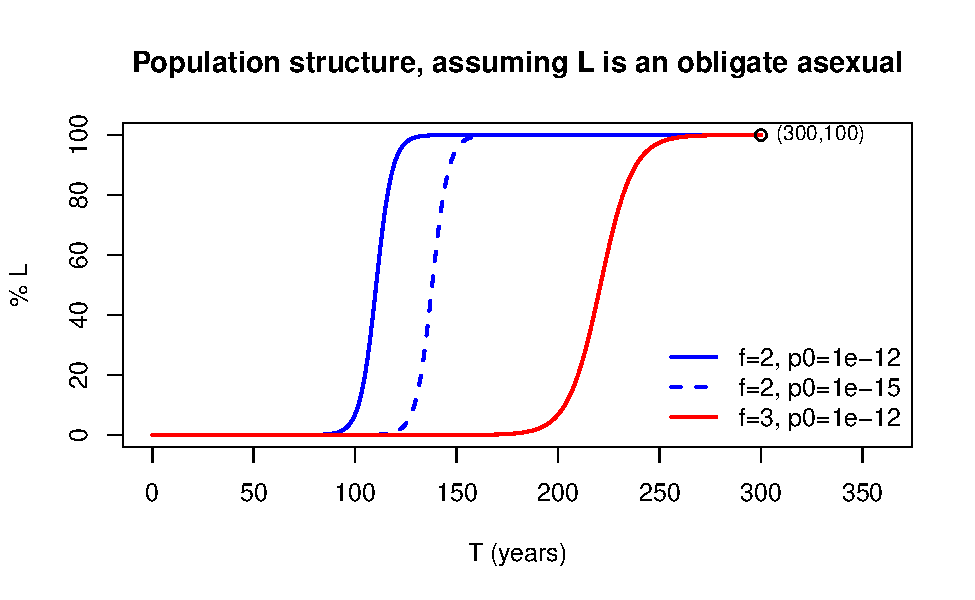
\includegraphics[width=\maxwidth]{asex-figs-knitr/asex-is-exponential-1} 

}



\end{knitrout}

[A tangent on p0: Here's a very crude estimate of global thaps population.  Assuming phytoplankton
are largely confined to the top 10 meters of the ocean (a volume of $3.4 \times 10^{18}$ liters),
and an average density of 10 cells per liter (you said ``thousands'' per liter in bloom conditions),
gives $3\times10^{19}$ cells:

\begin{knitrout}\footnotesize
\definecolor{shadecolor}{rgb}{0.969, 0.969, 0.969}\color{fgcolor}\begin{kframe}
\begin{alltt}
\hlstd{r}   \hlkwb{<-} \hlnum{6371000}              \hlcom{# radius of earth (m)}
\hlstd{A}   \hlkwb{<-} \hlnum{2}\hlopt{/}\hlnum{3}\hlopt{*}\hlnum{4}\hlopt{*}\hlstd{pi}\hlopt{*}\hlstd{r}\hlopt{^}\hlnum{2}         \hlcom{# area of oceans (m^2)}
\hlstd{V}   \hlkwb{<-} \hlstd{A} \hlopt{*} \hlnum{10} \hlopt{*} \hlnum{100}\hlopt{^}\hlnum{3}\hlopt{/}\hlnum{1000}  \hlcom{# liters of sea water within 10m of surface}
\hlstd{cpl} \hlkwb{<-} \hlnum{10}                   \hlcom{# cells per liter (non-bloom)}
\hlkwd{cat}\hlstd{(}\hlstr{">> Est."}\hlstd{,} \hlkwd{signif}\hlstd{(}\hlnum{10}\hlopt{*}\hlstd{V,}\hlnum{1}\hlstd{),} \hlstr{'cells, assuming global avg of'}\hlstd{, cpl,}
    \hlstr{'cells per L (non-bloom) x'}\hlstd{,} \hlkwd{signif}\hlstd{(V,}\hlnum{2}\hlstd{),} \hlstr{'liters.\textbackslash{}n'}\hlstd{)}
\end{alltt}
\begin{verbatim}
# >> Est. 3e+19 cells, assuming global avg of 10 cells per L (non-bloom) x 3.4e+18 liters.
\end{verbatim}
\end{kframe}
\end{knitrout}

By this estimate, perhaps I should set $p0\approx 10^{-19}$. Again, this could be way off and please
correct if so, but I don't think it will fundamentally change the picture---as noted in the first
simulation, dropping the initial proportion a thousand fold only adds a few decades to the time
line, and I think the early stages of growth from a single ancestral L cell will be dominated by
stochastic effects, anyway, i.e., my growth model above is most appropriate after L has reached a
scale, say millions of cells, where stochastic effects are minor.]

\section{Model 2: \textit{Slowed} sexual reproduction \textit{also} = exponential growth advantage}
\label{sec:slowexpo}

Instead of obligate asexuality, what if L just had a reduced rate of meiosis?  E.g., $b_x=0.2$ in
comparison to non-L's $b_y=0.5$?  The result is almost the same: L will grow to dominate the global
population in only a few hundred years.  There is, however, one important twist---in this model, in
the limit, L's proportion of the population is \textit{not} 100\%, for the reason that the large L
population is continually creating sexual offspring that are recognizably non-L (as we've discussed
before).  But if we assume for now (but see next section) that these non-L cells undergo meiosis at
the non-L rate $b_y$, then asexual growth in L holds the clonal lineage at a high level.

Modeling here is similar to that outlined in the previous section.  The key difference is that in
each epoch we assume that a fraction $\beta_x = b_x/(a/k)$ of the L population undergoes meiosis,
while $(1-\beta_x)$ divides mitotically $k$ times in one epoch, as before.  Also, the meiotic
offspring of L are added to the \textit{non-L} proportion of the population; this change has little
effect while the L proportion is small, but serves to keep the non-L proportion from shrinking to
zero after L becomes dominant.  Again we are assuming both the L and non-L populations are on
average adequately characterized by the parameters $a,k,f,b_x,$ and $b_y$, which implies no fitness
differences other than the different meiotic rates.

\begin{knitrout}\footnotesize
\definecolor{shadecolor}{rgb}{0.969, 0.969, 0.969}\color{fgcolor}\begin{kframe}
\begin{alltt}
\hlcom{# grow2 simulates 'yrs' years of growth in the 2-component model where L & non-L  }
\hlcom{# have equal mitotic but unequal meiotic rates.}
\hlstd{grow2} \hlkwb{<-} \hlkwa{function}\hlstd{(}\hlkwc{yrs}\hlstd{,} \hlkwc{a}\hlstd{=}\hlnum{180}\hlstd{,} \hlkwc{bx}\hlstd{=}\hlnum{0.2}\hlstd{,} \hlkwc{by}\hlstd{=}\hlnum{0.5}\hlstd{,} \hlkwc{k}\hlstd{=}\hlnum{2}\hlstd{,} \hlkwc{f}\hlstd{=}\hlnum{2}\hlstd{,} \hlkwc{p0}\hlstd{=}\hlnum{1e-12}\hlstd{)\{}
  \hlstd{n} \hlkwb{<-} \hlkwd{round}\hlstd{(yrs}\hlopt{*}\hlstd{a}\hlopt{/}\hlstd{k)} \hlcom{# number of epochs to simulate}
  \hlstd{x} \hlkwb{<-} \hlkwd{numeric}\hlstd{(n)}     \hlcom{# proportion in L}
  \hlstd{y} \hlkwb{<-} \hlkwd{numeric}\hlstd{(n)}     \hlcom{# proportion non-L}
  \hlstd{betax} \hlkwb{<-} \hlstd{bx}\hlopt{/}\hlstd{(a}\hlopt{/}\hlstd{k)}   \hlcom{# meioses per epoch in L}
  \hlstd{betay} \hlkwb{<-} \hlstd{by}\hlopt{/}\hlstd{(a}\hlopt{/}\hlstd{k)}   \hlcom{# meioses per epoch in non-L}
  \hlstd{x[}\hlnum{1}\hlstd{]} \hlkwb{<-} \hlstd{p0}          \hlcom{# initial proportion in L}
  \hlstd{y[}\hlnum{1}\hlstd{]} \hlkwb{<-} \hlnum{1}\hlopt{-}\hlstd{x[}\hlnum{1}\hlstd{]}
  \hlkwa{for}\hlstd{(i} \hlkwa{in} \hlnum{2}\hlopt{:}\hlstd{n)\{}
    \hlcom{# L grows mitotically:}
    \hlstd{x[i]} \hlkwb{<-} \hlstd{x[i}\hlopt{-}\hlnum{1}\hlstd{]}\hlopt{*}\hlstd{(}\hlnum{1}\hlopt{-}\hlstd{betax)}\hlopt{*}\hlnum{2}\hlopt{^}\hlstd{k}
    \hlcom{# non-L grows both ways \textbackslash{}textit\{and\} absorbs meiotic offspring of L}
    \hlstd{y[i]} \hlkwb{<-} \hlstd{x[i}\hlopt{-}\hlnum{1}\hlstd{]}\hlopt{*}\hlstd{betax}\hlopt{*}\hlstd{f} \hlopt{+} \hlstd{y[i}\hlopt{-}\hlnum{1}\hlstd{]}\hlopt{*}\hlstd{((}\hlnum{1}\hlopt{-}\hlstd{betay)}\hlopt{*}\hlnum{2}\hlopt{^}\hlstd{k} \hlopt{+} \hlstd{betay}\hlopt{*}\hlstd{f)}
    \hlstd{x[i]} \hlkwb{<-} \hlstd{x[i]}\hlopt{/}\hlstd{(x[i]}\hlopt{+}\hlstd{y[i])}  \hlcom{# re-normalize}
    \hlstd{y[i]} \hlkwb{<-} \hlnum{1}\hlopt{-}\hlstd{x[i]}            \hlcom{# re-normalize}
  \hlstd{\}}
  \hlstd{t} \hlkwb{<-} \hlstd{(}\hlnum{0}\hlopt{:}\hlstd{(n}\hlopt{-}\hlnum{1}\hlstd{))}\hlopt{/}\hlstd{a}\hlopt{*}\hlstd{k}  \hlcom{# rescale epoch numbers to years}
  \hlkwd{return}\hlstd{(}\hlkwd{list}\hlstd{(}\hlkwc{x}\hlstd{=x,} \hlkwc{y}\hlstd{=y,} \hlkwc{t}\hlstd{=t))}
\hlstd{\}}
\end{alltt}
\end{kframe}
\end{knitrout}

The three examples shown below illustrate hypothetical meiosis in L never, every 10 years and every
5 years, all in comparison to every 2 years in non-L.  As seen in the graphs below, reducing the
difference in meiotic rate between L and non-L delays L's transition and lowers its asymptotic
proportion, but the general trends are qualitatively the same---L rises from 1 part per trillion to
a large fraction of the population in a few centuries.  (A fourth, yellow, curve was also plotted,
based on the ``grow1'' asexual simulation given earlier, but this curve is \textit{completely}
overlaid by the blue $b_x=0$ curve from ``grow2''. This is expected, since the second model with
$b_x=0$ is logically equivalent to the first model; I included it as a sanity check.)

\begin{knitrout}\footnotesize
\definecolor{shadecolor}{rgb}{0.969, 0.969, 0.969}\color{fgcolor}\begin{kframe}
\begin{alltt}
\hlcom{# plot a few examples}
\hlstd{growex2} \hlkwb{<-} \hlkwa{function}\hlstd{(}\hlkwc{yrs}\hlstd{=}\hlnum{700}\hlstd{,} \hlkwc{a}\hlstd{=}\hlnum{180}\hlstd{,} \hlkwc{bx}\hlstd{=}\hlnum{0.2}\hlstd{,} \hlkwc{by}\hlstd{=}\hlnum{0.5}\hlstd{,} \hlkwc{k}\hlstd{=}\hlnum{2}\hlstd{,} \hlkwc{f}\hlstd{=}\hlnum{2}\hlstd{,} \hlkwc{p0}\hlstd{=}\hlnum{1e-12}\hlstd{)\{}
  \hlcom{# Set up plot axes }
  \hlkwd{plot}\hlstd{(}\hlkwa{NULL}\hlstd{,}\hlkwc{type}\hlstd{=}\hlstr{'n'}\hlstd{,} \hlkwc{xlim}\hlstd{=}\hlkwd{c}\hlstd{(}\hlnum{0}\hlstd{,}\hlnum{1.2}\hlopt{*}\hlstd{yrs),} \hlkwc{ylim}\hlstd{=}\hlkwd{c}\hlstd{(}\hlnum{0}\hlstd{,}\hlnum{100}\hlstd{),} \hlkwc{xlab}\hlstd{=}\hlstr{'T (years)'}\hlstd{,} \hlkwc{ylab}\hlstd{=}\hlstr{'% L'}\hlstd{,}
        \hlkwc{main}\hlstd{=}\hlstr{'Population structure, assuming L is occasionally sexual'}\hlstd{)}
  \hlstd{asex}  \hlkwb{<-} \hlkwd{grow1}\hlstd{(yrs, a,         by, k, f, p0)} \hlcom{# *a*sex simulation w/ default params}
  \hlstd{sex00} \hlkwb{<-} \hlkwd{grow2}\hlstd{(yrs, a,} \hlkwc{bx}\hlstd{=}\hlnum{0.0}\hlstd{, by, k, f, p0)} \hlcom{# sanity check: new w/ bx=0 should = old}
  \hlstd{sex01} \hlkwb{<-} \hlkwd{grow2}\hlstd{(yrs, a,} \hlkwc{bx}\hlstd{=}\hlnum{0.1}\hlstd{, by, k, f, p0)} \hlcom{# sim w/ more sexual offspring}
  \hlstd{sex02} \hlkwb{<-} \hlkwd{grow2}\hlstd{(yrs, a,} \hlkwc{bx}\hlstd{=}\hlnum{0.2}\hlstd{, by, k, f, p0)} \hlcom{# sim w/ even more}
  \hlkwd{plot1}\hlstd{(asex,}  \hlstr{'yellow'}\hlstd{)}
  \hlkwd{plot1}\hlstd{(sex00,} \hlstr{'blue'}\hlstd{)}
  \hlkwd{plot1}\hlstd{(sex01,} \hlstr{'darkgreen'}\hlstd{)}
  \hlkwd{plot1}\hlstd{(sex02,} \hlstr{'red'}\hlstd{)}
  \hlkwd{legend}\hlstd{(}\hlstr{'bottomright'}\hlstd{,}
         \hlkwc{legend}\hlstd{=}\hlkwd{c}\hlstd{(}\hlstr{'bx=0.0, by=0.5'}\hlstd{,} \hlstr{'bx=0.1, by=0.5'}\hlstd{,} \hlstr{'bx=0.2, by=0.5'}\hlstd{),}
         \hlkwc{col}\hlstd{=}   \hlkwd{c}\hlstd{(}\hlstr{'blue'}\hlstd{,}           \hlstr{'darkgreen'}\hlstd{,}      \hlstr{'red'}\hlstd{),}
         \hlkwc{lwd}\hlstd{=}\hlnum{2}\hlstd{,} \hlkwc{bty}\hlstd{=}\hlstr{'n'}\hlstd{)}
\hlstd{\}}
\end{alltt}
\end{kframe}
\end{knitrout}

\begin{knitrout}\footnotesize
\definecolor{shadecolor}{rgb}{0.969, 0.969, 0.969}\color{fgcolor}\begin{kframe}
\begin{alltt}
\hlkwd{growex2}\hlstd{()}
\end{alltt}
\end{kframe}

{\centering \includegraphics[width=\maxwidth]{asex-figs-knitr/slow-sex-is-exponential-1} 

}



\end{knitrout}

(Once L becomes dominant in the population, its meiotic offspring frequently will be consanguineous,
including direct L cross L matings.  Inbreeding-depression might reduce the non-L proportion of the
population, but this effect seems insufficiently strong to eliminate the non-L population,
especially given that we believe L itself to be inbred.)

So, superficially, this model is plausibly consistent with our observations \textit{without}
mandating that L is an obligate asexual; it just requires that L undergoes meoisis less frequently
(coupled with meiosis being less ``productive'' than mitosis, due to longer cell division times,
incomplete fertilization, etc., all of which are expected).  However, in these models the non-L
populations largely will be descendants of L, so it is not clear that they could maintain the large
pool of non-L SNPs that we see in both H isolates.  This is more fully explored in
Section~\ref{sec:offspring}.

Furthermore, after allowing for what I think is the most plausible genetic explanation for reduced
meiotic frequency, I think obligate asexual is the most likely scenario: see Section~\ref{sec:smr}.

\section{Tracking L's offspring}
\label{sec:offspring}

Summarizing some of the above thoughts: the offspring of a facultative sexual share genes with their
parents, but are distinct from it.  A \emph{plentiful clone} that is facultatively sexual thus
pushes \emph{many copies} of the clonal sequences into the remaining population.  This section begins
to model that; the results in Section~\ref{sec:hitchhiking} repeat this in a more general way.

\subsection{Model 2-prime: Tracking L's offspring}
\label{sec:2prime}

In the ``slow sex'' model considered in the previous section, the sexual offspring of L carry
L-alleles into the non-L population.  The extent of this admixture is explored in this section.
Somewhat surprisingly, this happend to an extreme extent, sufficiently so that the stable L/non-L
coexistance depicted above cannot explain our observed L/H snapshot.  The simulations below first
consider only non-L cells that can trace all ancestors to L (e.g., a direct L-L cross, or crosses
between such crosses).  The second analysis drops this ``pure-L-ancestry'' restriction.  In
retrospect, the second analysis is the more interesting, but I'll leave the first just because I
thought of it first...

\begin{knitrout}\footnotesize
\definecolor{shadecolor}{rgb}{0.969, 0.969, 0.969}\color{fgcolor}\begin{kframe}
\begin{alltt}
\hlcom{# grow2 simulates 'yrs' years of growth in the 2-component model where L & non-L have}
\hlcom{# equal mitotic but inequal meiotic rates.  Additionally, track the proportion of the}
\hlcom{# population that has purely L-ancestry (i.e., direct result of L-L crosses, of L crossing}
\hlcom{# with them and with each other, etc.).  The later are assumed to have the same meiotic}
\hlcom{# and mitotic rates as other non-L genotype, but would be genetically recognizable due to}
\hlcom{# their near-absence of non-reference nucleotides not seen in L. Plot later as dashed line}
\hlcom{# atop L portion.}
\hlstd{grow2pold} \hlkwb{<-} \hlkwa{function}\hlstd{(}\hlkwc{yrs}\hlstd{,} \hlkwc{a}\hlstd{=}\hlnum{180}\hlstd{,} \hlkwc{bx}\hlstd{=}\hlnum{0.2}\hlstd{,} \hlkwc{by}\hlstd{=}\hlnum{0.5}\hlstd{,} \hlkwc{k}\hlstd{=}\hlnum{2}\hlstd{,} \hlkwc{f}\hlstd{=}\hlnum{2}\hlstd{,} \hlkwc{p0}\hlstd{=}\hlnum{1e-12}\hlstd{)\{}
  \hlstd{n}  \hlkwb{<-} \hlkwd{round}\hlstd{(yrs}\hlopt{*}\hlstd{a}\hlopt{/}\hlstd{k)} \hlcom{# number of epochs to simulate}
  \hlstd{x}  \hlkwb{<-} \hlkwd{numeric}\hlstd{(n)}     \hlcom{# proportion in L}
  \hlstd{z}  \hlkwb{<-} \hlkwd{numeric}\hlstd{(n)}     \hlcom{# proportion in LxL}
  \hlstd{y}  \hlkwb{<-} \hlkwd{numeric}\hlstd{(n)}     \hlcom{# proportion other non-L}
  \hlstd{betax} \hlkwb{<-} \hlstd{bx}\hlopt{/}\hlstd{(a}\hlopt{/}\hlstd{k)}    \hlcom{# meioses per epoch in L}
  \hlstd{betay} \hlkwb{<-} \hlstd{by}\hlopt{/}\hlstd{(a}\hlopt{/}\hlstd{k)}    \hlcom{# meioses per epoch in non-L}
  \hlstd{x[}\hlnum{1}\hlstd{]}  \hlkwb{<-} \hlstd{p0}          \hlcom{# initial proportion in L}
  \hlstd{z[}\hlnum{1}\hlstd{]}  \hlkwb{<-} \hlnum{0}
  \hlstd{y[}\hlnum{1}\hlstd{]}  \hlkwb{<-} \hlnum{1}\hlopt{-}\hlstd{x[}\hlnum{1}\hlstd{]}
  \hlkwa{for}\hlstd{(i} \hlkwa{in} \hlnum{2}\hlopt{:}\hlstd{n)\{}
    \hlcom{# total meiotic fraction}
    \hlstd{m} \hlkwb{<-} \hlstd{x[i}\hlopt{-}\hlnum{1}\hlstd{]}\hlopt{*}\hlstd{betax} \hlopt{+} \hlstd{(z[i}\hlopt{-}\hlnum{1}\hlstd{]}\hlopt{+}\hlstd{y[i}\hlopt{-}\hlnum{1}\hlstd{])}\hlopt{*}\hlstd{betay}
    \hlcom{# fraction of them that are purely-L-ancestory}
    \hlstd{p} \hlkwb{<-} \hlstd{(x[i}\hlopt{-}\hlnum{1}\hlstd{]}\hlopt{*}\hlstd{betax} \hlopt{+} \hlstd{z[i}\hlopt{-}\hlnum{1}\hlstd{]}\hlopt{*}\hlstd{betay)}\hlopt{/}\hlstd{m}
    \hlstd{q} \hlkwb{<-} \hlnum{1}\hlopt{-}\hlstd{p}
    \hlcom{# L grows mitotically:}
    \hlstd{x[i]}  \hlkwb{<-}  \hlstd{x[i}\hlopt{-}\hlnum{1}\hlstd{]}\hlopt{*}\hlstd{(}\hlnum{1}\hlopt{-}\hlstd{betax)}\hlopt{*}\hlnum{2}\hlopt{^}\hlstd{k}
    \hlcom{# non-L grows both ways *and* absorbs meiotic offspring }
    \hlcom{# of L, with p^2 fraction retaining L-purity}
    \hlstd{z[i]}  \hlkwb{<-} \hlstd{z[i}\hlopt{-}\hlnum{1}\hlstd{]}\hlopt{*}\hlstd{(}\hlnum{1}\hlopt{-}\hlstd{betay)}\hlopt{*}\hlnum{2}\hlopt{^}\hlstd{k} \hlopt{+}    \hlstd{p}\hlopt{^}\hlnum{2}  \hlopt{*} \hlstd{m} \hlopt{*} \hlstd{f}
    \hlstd{y[i]}  \hlkwb{<-} \hlstd{y[i}\hlopt{-}\hlnum{1}\hlstd{]}\hlopt{*}\hlstd{(}\hlnum{1}\hlopt{-}\hlstd{betay)}\hlopt{*}\hlnum{2}\hlopt{^}\hlstd{k} \hlopt{+} \hlstd{(}\hlnum{1}\hlopt{-}\hlstd{p}\hlopt{^}\hlnum{2}\hlstd{)} \hlopt{*} \hlstd{m} \hlopt{*} \hlstd{f}
    \hlstd{w} \hlkwb{<-} \hlstd{x[i]}\hlopt{+}\hlstd{z[i]}\hlopt{+}\hlstd{y[i]}
    \hlstd{x[i]}  \hlkwb{<-}  \hlstd{x[i]}\hlopt{/}\hlstd{w}    \hlcom{# re-normalize}
    \hlstd{z[i]}  \hlkwb{<-}  \hlstd{z[i]}\hlopt{/}\hlstd{w}    \hlcom{# re-normalize}
    \hlstd{y[i]}  \hlkwb{<-}  \hlstd{y[i]}\hlopt{/}\hlstd{w}    \hlcom{# re-normalize}
  \hlstd{\}}
  \hlstd{t} \hlkwb{<-} \hlstd{((}\hlnum{1}\hlopt{:}\hlstd{n)}\hlopt{-}\hlnum{1}\hlstd{)}\hlopt{/}\hlstd{a}\hlopt{*}\hlstd{k}  \hlcom{# rescale epoch numbers to years}
  \hlkwd{return}\hlstd{(}\hlkwd{list}\hlstd{(}\hlkwc{x}\hlstd{=x,} \hlkwc{z}\hlstd{=z,} \hlkwc{y}\hlstd{=y,} \hlkwc{t}\hlstd{=t))}
\hlstd{\}}
\end{alltt}
\end{kframe}
\end{knitrout}

\begin{knitrout}\footnotesize
\definecolor{shadecolor}{rgb}{0.969, 0.969, 0.969}\color{fgcolor}\begin{kframe}
\begin{alltt}
\hlcom{# plot2p plots a growth series g (as returned by grow2p) in specified color, line type}
\hlstd{plot2pold} \hlkwb{<-} \hlkwa{function}\hlstd{(}\hlkwc{g}\hlstd{,}\hlkwc{col}\hlstd{,}\hlkwc{lty}\hlstd{=}\hlnum{1}\hlstd{,} \hlkwc{label}\hlstd{=F)\{}
  \hlstd{n} \hlkwb{<-} \hlkwd{length}\hlstd{(g}\hlopt{$}\hlstd{x)}
  \hlstd{p} \hlkwb{<-} \hlstd{g}\hlopt{$}\hlstd{x} \hlopt{*} \hlnum{100}                          \hlcom{# rescale x to percent}
  \hlkwd{lines}\hlstd{(g}\hlopt{$}\hlstd{t, p,} \hlkwc{lwd}\hlstd{=}\hlnum{2}\hlstd{,} \hlkwc{col}\hlstd{=col,} \hlkwc{lty}\hlstd{=lty)}  \hlcom{# plot x vs t}
  \hlkwd{showxy}\hlstd{(g}\hlopt{$}\hlstd{t[n], p[n])}                    \hlcom{# annotate last point in series}
  \hlcom{# now plot growth of z atop x as a thinner dashed line. (plot subseq of about 100}
  \hlcom{# points,  otherwise dashing is obscured)}
  \hlstd{ss} \hlkwb{<-} \hlkwd{seq}\hlstd{(}\hlkwc{from}\hlstd{=}\hlnum{1}\hlstd{,} \hlkwc{to}\hlstd{=n,} \hlkwc{by}\hlstd{=}\hlkwd{ceiling}\hlstd{(n}\hlopt{/}\hlnum{100}\hlstd{))}
  \hlkwd{lines}\hlstd{(g}\hlopt{$}\hlstd{t[ss], (g}\hlopt{$}\hlstd{x[ss]}\hlopt{+}\hlstd{g}\hlopt{$}\hlstd{z[ss])}\hlopt{*}\hlnum{100}\hlstd{,} \hlkwc{lwd}\hlstd{=}\hlnum{1}\hlstd{,} \hlkwc{col}\hlstd{=col,} \hlkwc{lty}\hlstd{=}\hlstr{'dashed'}\hlstd{)}
  \hlkwa{if}\hlstd{(label)\{} \hlcom{# label last point in this one too?}
    \hlstd{pp} \hlkwb{<-} \hlstd{(g}\hlopt{$}\hlstd{x[n]}\hlopt{+}\hlstd{g}\hlopt{$}\hlstd{z[n])}\hlopt{*}\hlnum{100}
    \hlstd{dy} \hlkwb{<-} \hlkwd{ifelse}\hlstd{(pp} \hlopt{<} \hlnum{50}\hlstd{,} \hlnum{3}\hlstd{,} \hlnum{0}\hlstd{)} \hlcom{# hack to avoid label collision for small pp }
    \hlkwd{showxy}\hlstd{(g}\hlopt{$}\hlstd{t[n],pp,} \hlkwc{dy}\hlstd{=dy,} \hlkwc{show.point}\hlstd{=}\hlnum{FALSE}\hlstd{)}
  \hlstd{\}}
\hlstd{\}}
\end{alltt}
\end{kframe}
\end{knitrout}

\begin{knitrout}\footnotesize
\definecolor{shadecolor}{rgb}{0.969, 0.969, 0.969}\color{fgcolor}\begin{kframe}
\begin{alltt}
\hlcom{# plot a few examples}
\hlstd{growex2pold} \hlkwb{<-} \hlkwa{function}\hlstd{(}\hlkwc{yrs}\hlstd{=}\hlnum{700}\hlstd{,} \hlkwc{a}\hlstd{=}\hlnum{180}\hlstd{,} \hlkwc{bx}\hlstd{=}\hlnum{0.2}\hlstd{,} \hlkwc{by}\hlstd{=}\hlnum{0.5}\hlstd{,} \hlkwc{k}\hlstd{=}\hlnum{2}\hlstd{,} \hlkwc{f}\hlstd{=}\hlnum{2}\hlstd{,} \hlkwc{p0}\hlstd{=}\hlnum{1e-12}\hlstd{)\{}
  \hlcom{# Set up plot axes }
  \hlkwd{plot}\hlstd{(}\hlkwa{NULL}\hlstd{,}\hlkwc{type}\hlstd{=}\hlstr{'n'}\hlstd{,} \hlkwc{xlim}\hlstd{=}\hlkwd{c}\hlstd{(}\hlnum{0}\hlstd{,}\hlnum{1.2}\hlopt{*}\hlstd{yrs),} \hlkwc{ylim}\hlstd{=}\hlkwd{c}\hlstd{(}\hlnum{0}\hlstd{,}\hlnum{100}\hlstd{),} \hlkwc{xlab}\hlstd{=}\hlstr{'T (years)'}\hlstd{,} \hlkwc{ylab}\hlstd{=}\hlstr{'%'}\hlstd{,}
        \hlkwc{main}\hlstd{=}\hlstr{'Population structure, assuming L is occasionally sexual'}\hlstd{)}
  \hlstd{asex}  \hlkwb{<-} \hlkwd{grow1}\hlstd{(yrs, a,         by, k, f, p0)} \hlcom{# *a*sex simulation w/ default params}
  \hlstd{sex00} \hlkwb{<-} \hlkwd{grow2pold}\hlstd{(yrs, a,} \hlkwc{bx}\hlstd{=}\hlnum{0.0}\hlstd{, by, k, f, p0)} \hlcom{# sanity check: new+(bx=0) should = old}
  \hlstd{sex01} \hlkwb{<-} \hlkwd{grow2pold}\hlstd{(yrs, a,} \hlkwc{bx}\hlstd{=}\hlnum{0.1}\hlstd{, by, k, f, p0)} \hlcom{# sim w/ more sexual offspring}
  \hlstd{sex02} \hlkwb{<-} \hlkwd{grow2pold}\hlstd{(yrs, a,} \hlkwc{bx}\hlstd{=}\hlnum{0.2}\hlstd{, by, k, f, p0)} \hlcom{# sim w/ even more}
  \hlcom{#sex022<- grow2pold(yrs, a, bx=0.22, by, k, f, p0) # sim w/ even more}
  \hlkwd{plot1}\hlstd{(asex,}  \hlstr{'yellow'}\hlstd{)}
  \hlkwd{plot2pold}\hlstd{(sex00,} \hlstr{'blue'}\hlstd{)}
  \hlkwd{plot2pold}\hlstd{(sex01,} \hlstr{'darkgreen'}\hlstd{,}\hlkwc{label}\hlstd{=T)}
  \hlkwd{plot2pold}\hlstd{(sex02,} \hlstr{'red'}\hlstd{,} \hlkwc{label}\hlstd{=T)}
  \hlkwd{legend}\hlstd{(}\hlstr{'bottomright'}\hlstd{,}
         \hlkwc{legend}\hlstd{=}\hlkwd{c}\hlstd{(}\hlstr{'%L: bx=0.0, by=0.5'}\hlstd{,} \hlstr{'%L: bx=0.1, by=0.5'}\hlstd{,} \hlstr{'%L: bx=0.2, by=0.5'}\hlstd{),}
         \hlkwc{col}\hlstd{=}   \hlkwd{c}\hlstd{(}\hlstr{'blue'}\hlstd{,}               \hlstr{'darkgreen'}\hlstd{,}          \hlstr{'red'}\hlstd{),}
         \hlkwc{lwd}\hlstd{=}\hlnum{2}\hlstd{,} \hlkwc{bty}\hlstd{=}\hlstr{'n'}\hlstd{)}
\hlstd{\}}
\hlkwd{growex2pold}\hlstd{()}
\end{alltt}
\end{kframe}\begin{figure}

{\centering \includegraphics[width=\maxwidth]{asex-figs-knitr/unnamed-chunk-13-1} 

}

\caption[Dotted lines show the incremental addition of ``pure-L-ancestry'' atop L]{Dotted lines show the incremental addition of ``pure-L-ancestry'' atop L.}\label{fig:unnamed-chunk-13}
\end{figure}


\end{knitrout}

Now look at overall allele frequencies in the whole non-L population.

\begin{knitrout}\footnotesize
\definecolor{shadecolor}{rgb}{0.969, 0.969, 0.969}\color{fgcolor}\begin{kframe}
\begin{alltt}
\hlcom{# In addition to the functionality of grow2pold above, this version tracks the allele }
\hlcom{# frequency, in the non-L-, non-pure-L-population, of any allele that is }
\hlcom{# identical-by-descent to an allele in L.  E.g., at a position that is polymorphic across }
\hlcom{# the initial L/non-L pop, does growth of L also push the L-alleles out into the non-L }
\hlcom{# population?  The reason to focus on identical-by-descent is that I can't estimate freq }
\hlcom{# of these alleles in the initial non-L pop, but finding IBD freq over time gives a lower }
\hlcom{# bound on overall freq. I do this separately for het and hom positions in L, i.e. initial}
\hlcom{# freq in L are exactly 1/2 or exactly 1.}
\hlcom{# }
\hlcom{# The variables "x, y, z", below, record (over time) the proportion of the population in}
\hlcom{# one of the following 3 genotype classes:}
\hlcom{#}
\hlcom{#   x: the L-genotype  }
\hlcom{#   z: non-L genotypes all of whose ancestors are traceable to L; e.g. (L x L) x L}
\hlcom{#   y: all other non-L (e.g., original wildtypes and L-outcrosses)}
\hlcom{# }
\hlcom{# Note that in x, all positions are either homozygous for the same nucleotide across all }
\hlcom{# cells, or heterozygous for the same pair of nucleotides across all cells.  In z, we will}
\hlcom{# see the same allele frequencies *on average*, but the 50:50 positions will exist in HWE}
\hlcom{# --- 25% homozygous for one allele, 25% hom for the other and 50% het.  In y, which is }
\hlcom{# initially all but p0, we could see any allele frequencies.  A question of interest, in }
\hlcom{# the case that x grows, is whether y can retain unique allele frequencies or whether }
\hlcom{# outcrossing of x and z with y will push y's allele frequency structure to become more }
\hlcom{# L-like.  This simulation suggests that yes, this happens.}
\hlstd{grow2p} \hlkwb{<-} \hlkwa{function}\hlstd{(}\hlkwc{yrs}\hlstd{,} \hlkwc{a}\hlstd{=}\hlnum{180}\hlstd{,} \hlkwc{bx}\hlstd{=}\hlnum{0.2}\hlstd{,} \hlkwc{by}\hlstd{=}\hlnum{0.5}\hlstd{,} \hlkwc{k}\hlstd{=}\hlnum{2}\hlstd{,} \hlkwc{f}\hlstd{=}\hlnum{2}\hlstd{,} \hlkwc{p0}\hlstd{=}\hlnum{1e-12}\hlstd{)\{}
  \hlstd{n}   \hlkwb{<-} \hlkwd{round}\hlstd{(yrs}\hlopt{*}\hlstd{a}\hlopt{/}\hlstd{k)}\hlcom{# number of epochs to simulate}
  \hlstd{x}   \hlkwb{<-} \hlkwd{numeric}\hlstd{(n)}    \hlcom{# proportion in L}
  \hlstd{z}   \hlkwb{<-} \hlkwd{numeric}\hlstd{(n)}    \hlcom{# proportion in LxL}
  \hlstd{y}   \hlkwb{<-} \hlkwd{numeric}\hlstd{(n)}    \hlcom{# proportion other non-L}
  \hlstd{y05} \hlkwb{<-} \hlkwd{numeric}\hlstd{(n)}    \hlcom{# allele freq IBD-from-L in non-L pop for a het position in L}
  \hlstd{y10} \hlkwb{<-} \hlkwd{numeric}\hlstd{(n)}    \hlcom{# allele freq IBD-from-L in non-L pop for a hom position in L}
  \hlstd{betax} \hlkwb{<-} \hlstd{bx}\hlopt{/}\hlstd{(a}\hlopt{/}\hlstd{k)}    \hlcom{# meioses per epoch in L}
  \hlstd{betay} \hlkwb{<-} \hlstd{by}\hlopt{/}\hlstd{(a}\hlopt{/}\hlstd{k)}    \hlcom{# meioses per epoch in non-L}
  \hlstd{x[}\hlnum{1}\hlstd{]}  \hlkwb{<-} \hlstd{p0}          \hlcom{# initial proportion in L}
  \hlstd{z[}\hlnum{1}\hlstd{]}  \hlkwb{<-} \hlnum{0}
  \hlstd{y[}\hlnum{1}\hlstd{]}  \hlkwb{<-} \hlnum{1}\hlopt{-}\hlstd{x[}\hlnum{1}\hlstd{]}
  \hlstd{y05[}\hlnum{1}\hlstd{]} \hlkwb{<-} \hlnum{0}
  \hlstd{y10[}\hlnum{1}\hlstd{]} \hlkwb{<-} \hlnum{0}
  \hlkwa{for}\hlstd{(i} \hlkwa{in} \hlnum{2}\hlopt{:}\hlstd{n)\{}
    \hlcom{# total meiotic fraction}
    \hlstd{m} \hlkwb{<-} \hlstd{x[i}\hlopt{-}\hlnum{1}\hlstd{]}\hlopt{*}\hlstd{betax} \hlopt{+} \hlstd{(z[i}\hlopt{-}\hlnum{1}\hlstd{]}\hlopt{+}\hlstd{y[i}\hlopt{-}\hlnum{1}\hlstd{])}\hlopt{*}\hlstd{betay}
    \hlcom{# fraction of them that are purely-L-ancestory}
    \hlstd{p} \hlkwb{<-} \hlstd{(x[i}\hlopt{-}\hlnum{1}\hlstd{]}\hlopt{*}\hlstd{betax} \hlopt{+} \hlstd{z[i}\hlopt{-}\hlnum{1}\hlstd{]}\hlopt{*}\hlstd{betay)}\hlopt{/}\hlstd{m}
    \hlstd{q} \hlkwb{<-} \hlnum{1}\hlopt{-}\hlstd{p}
    \hlcom{# L grows only mitotically:}
    \hlstd{x[i]}  \hlkwb{<-}  \hlstd{x[i}\hlopt{-}\hlnum{1}\hlstd{]}\hlopt{*}\hlstd{(}\hlnum{1}\hlopt{-}\hlstd{betax)}\hlopt{*}\hlnum{2}\hlopt{^}\hlstd{k}
    \hlcom{# non-L grows both ways *and* absorbs meiotic offspring }
    \hlcom{# of L, with p^2 fraction retaining L-purity}
    \hlstd{z[i]} \hlkwb{<-} \hlstd{z[i}\hlopt{-}\hlnum{1}\hlstd{]}\hlopt{*}\hlstd{(}\hlnum{1}\hlopt{-}\hlstd{betay)}\hlopt{*}\hlnum{2}\hlopt{^}\hlstd{k} \hlopt{+}    \hlstd{p}\hlopt{^}\hlnum{2}  \hlopt{*} \hlstd{m} \hlopt{*} \hlstd{f}
    \hlstd{y[i]} \hlkwb{<-} \hlstd{y[i}\hlopt{-}\hlnum{1}\hlstd{]}\hlopt{*}\hlstd{(}\hlnum{1}\hlopt{-}\hlstd{betay)}\hlopt{*}\hlnum{2}\hlopt{^}\hlstd{k} \hlopt{+} \hlstd{(}\hlnum{1}\hlopt{-}\hlstd{p}\hlopt{^}\hlnum{2}\hlstd{)} \hlopt{*} \hlstd{m} \hlopt{*} \hlstd{f}
    \hlcom{# Tracking L's introgression into y's allele frequency structure: Consider one epoch. }
    \hlcom{# Picture x,y,z as cell *counts* in the population (in units of the total pop size if }
    \hlcom{# you prefer). Count chromosomes (2 per cell, of course) being added to y's gene pool}
    \hlcom{# as a result of both mitosis and meiosis of y cells, and meiosis of x and z cells. }
    \hlcom{# (Mitosis within x and z don't contribute to y.)  Oh, rats -- I really should have}
    \hlcom{# said "count physical copies of one haploid genome, of which there are 2 per cell",}
    \hlcom{# but I don't want to change many variable names and comments at this late stage, so}
    \hlcom{# just pretend that "ch" is somehow an abbreviation for "copies, haplo" or somehing,}
    \hlcom{# and that "chromosome" in many of the comments below really means "haplocopy".}
    \hlstd{ch.y.mito} \hlkwb{<-} \hlstd{y[i}\hlopt{-}\hlnum{1}\hlstd{]} \hlopt{*} \hlstd{(}\hlnum{1}\hlopt{-}\hlstd{betay)} \hlopt{*} \hlnum{2}\hlopt{^}\hlstd{k} \hlopt{*} \hlnum{2}
    \hlstd{ch.y.meio} \hlkwb{<-} \hlstd{y[i}\hlopt{-}\hlnum{1}\hlstd{]} \hlopt{*} \hlstd{betay} \hlopt{*} \hlstd{f} \hlopt{*} \hlnum{2}
    \hlstd{ch.z.meio} \hlkwb{<-} \hlstd{z[i}\hlopt{-}\hlnum{1}\hlstd{]} \hlopt{*} \hlstd{betay} \hlopt{*} \hlstd{f} \hlopt{*} \hlnum{2}
    \hlstd{ch.x.meio} \hlkwb{<-} \hlstd{x[i}\hlopt{-}\hlnum{1}\hlstd{]} \hlopt{*} \hlstd{betax} \hlopt{*} \hlstd{f} \hlopt{*} \hlnum{2}
    \hlcom{# New freq in y at L's het sites: Initially, y dominates the population, and nearly}
    \hlcom{# all chromosomes in the y gene pool in one epoch come from meiosis and, especially,}
    \hlcom{# mitosis of y cells.  Whatever past introgression of L alleles has occurred is}
    \hlcom{# measured by y05[] and y10[], and these (initially tiny fractions) are}
    \hlcom{# proportionately carried forward into the next epoch.  In contrast, chromosomes being}
    \hlcom{# added to y that originate from meioses in x or z carry L alleles at L frequencies,}
    \hlcom{# i.e. 1/2 or 1.  The y05 and y10 values for the next epoch are simply a weighted}
    \hlcom{# average of these contributions.  Although the number of chromosomes contributed by}
    \hlcom{# x/z is initially small, these allele frequecies are large and seem to inexorably}
    \hlcom{# build in the population, especially as x/z grow.}
    \hlstd{y05[i]} \hlkwb{<-} \hlstd{((ch.y.mito} \hlopt{+} \hlstd{ch.y.meio)} \hlopt{*} \hlstd{y05[i}\hlopt{-}\hlnum{1}\hlstd{]} \hlopt{+} \hlstd{(ch.z.meio} \hlopt{+} \hlstd{ch.x.meio)} \hlopt{*} \hlnum{0.5}\hlstd{)} \hlopt{/}
              \hlstd{( ch.y.mito} \hlopt{+} \hlstd{ch.y.meio}             \hlopt{+}  \hlstd{ch.z.meio} \hlopt{+} \hlstd{ch.x.meio       )}
    \hlstd{y10[i]} \hlkwb{<-} \hlstd{((ch.y.mito} \hlopt{+} \hlstd{ch.y.meio)} \hlopt{*} \hlstd{y10[i}\hlopt{-}\hlnum{1}\hlstd{]} \hlopt{+} \hlstd{(ch.z.meio} \hlopt{+} \hlstd{ch.x.meio)} \hlopt{*} \hlnum{1.0}\hlstd{)} \hlopt{/}
              \hlstd{( ch.y.mito} \hlopt{+} \hlstd{ch.y.meio}             \hlopt{+}  \hlstd{ch.z.meio} \hlopt{+} \hlstd{ch.x.meio       )}
    \hlstd{w} \hlkwb{<-} \hlstd{x[i]}\hlopt{+}\hlstd{z[i]}\hlopt{+}\hlstd{y[i]}
    \hlstd{x[i]} \hlkwb{<-} \hlstd{x[i]}\hlopt{/}\hlstd{w}    \hlcom{# re-normalize}
    \hlstd{z[i]} \hlkwb{<-} \hlstd{z[i]}\hlopt{/}\hlstd{w}    \hlcom{# re-normalize}
    \hlstd{y[i]} \hlkwb{<-} \hlstd{y[i]}\hlopt{/}\hlstd{w}    \hlcom{# re-normalize}
  \hlstd{\}}
  \hlcom{# in retrospect, no need to compute y10; it's always twice y05.  Easily seen by}
  \hlcom{# induction on i at defining calculation above or by:}
  \hlkwa{if}\hlstd{(}\hlkwd{max}\hlstd{(}\hlkwd{abs}\hlstd{(y10} \hlopt{-} \hlnum{2}\hlopt{*}\hlstd{y05))}\hlopt{>}\hlnum{1e-12}\hlstd{)\{}
    \hlkwd{print}\hlstd{(}\hlkwd{summary}\hlstd{(y10}\hlopt{-}\hlnum{2}\hlopt{*}\hlstd{y05))}
  \hlstd{\}}
  \hlstd{t} \hlkwb{<-} \hlstd{((}\hlnum{1}\hlopt{:}\hlstd{n)}\hlopt{-}\hlnum{1}\hlstd{)}\hlopt{/}\hlstd{a}\hlopt{*}\hlstd{k}  \hlcom{# rescale epoch numbers to years}
  \hlkwd{return}\hlstd{(}\hlkwd{list}\hlstd{(}\hlkwc{x}\hlstd{=x,} \hlkwc{z}\hlstd{=z,} \hlkwc{y}\hlstd{=y,} \hlkwc{y05}\hlstd{=y05,} \hlkwc{y10}\hlstd{=y10,} \hlkwc{t}\hlstd{=t))}
\hlstd{\}}
\end{alltt}
\end{kframe}
\end{knitrout}

\begin{knitrout}\footnotesize
\definecolor{shadecolor}{rgb}{0.969, 0.969, 0.969}\color{fgcolor}\begin{kframe}
\begin{alltt}
\hlcom{# plot2p plots a growth series g (as returned by grow2p) in specified color, line type}
\hlstd{plot2p} \hlkwb{<-} \hlkwa{function}\hlstd{(}\hlkwc{g}\hlstd{,}\hlkwc{col}\hlstd{,}\hlkwc{lty}\hlstd{=}\hlnum{1}\hlstd{,} \hlkwc{label}\hlstd{=F)\{}
  \hlstd{n} \hlkwb{<-} \hlkwd{length}\hlstd{(g}\hlopt{$}\hlstd{x)}
  \hlstd{p} \hlkwb{<-} \hlstd{g}\hlopt{$}\hlstd{x} \hlopt{*} \hlnum{100}                          \hlcom{# rescale x to percent}
  \hlkwd{lines}\hlstd{(g}\hlopt{$}\hlstd{t, p,} \hlkwc{lwd}\hlstd{=}\hlnum{2}\hlstd{,} \hlkwc{col}\hlstd{=col,} \hlkwc{lty}\hlstd{=lty)}  \hlcom{# plot x vs t}
  \hlkwd{showxy}\hlstd{(g}\hlopt{$}\hlstd{t[n], p[n])}                    \hlcom{# annotate last point in series}
  \hlcom{# now plot growth of z atop x as a thinner dashed line, and y05, y10 as dotted, }
  \hlcom{# dash-dotted, resp. (plot subseq of about 100 points for these, otherwise dash/dot is }
  \hlcom{# obscured)}
  \hlstd{ss} \hlkwb{<-} \hlkwd{seq}\hlstd{(}\hlkwc{from}\hlstd{=}\hlnum{1}\hlstd{,} \hlkwc{to}\hlstd{=n,} \hlkwc{by}\hlstd{=}\hlkwd{ceiling}\hlstd{(n}\hlopt{/}\hlnum{100}\hlstd{))}
  \hlkwd{lines}\hlstd{(g}\hlopt{$}\hlstd{t[ss], (g}\hlopt{$}\hlstd{x[ss]}\hlopt{+}\hlstd{g}\hlopt{$}\hlstd{z[ss])}\hlopt{*}\hlnum{100}\hlstd{,} \hlkwc{lwd}\hlstd{=}\hlnum{1}\hlstd{,} \hlkwc{col}\hlstd{=col,} \hlkwc{lty}\hlstd{=}\hlstr{'dashed'}\hlstd{)}
  \hlkwd{lines}\hlstd{(g}\hlopt{$}\hlstd{t[ss], (g}\hlopt{$}\hlstd{y10[ss])}\hlopt{*}\hlnum{100}\hlstd{,} \hlkwc{lwd}\hlstd{=}\hlnum{1}\hlstd{,} \hlkwc{col}\hlstd{=col,} \hlkwc{lty}\hlstd{=}\hlstr{'dotdash'}\hlstd{)}
  \hlkwd{lines}\hlstd{(g}\hlopt{$}\hlstd{t[ss], (g}\hlopt{$}\hlstd{y05[ss])}\hlopt{*}\hlnum{100}\hlstd{,} \hlkwc{lwd}\hlstd{=}\hlnum{1}\hlstd{,} \hlkwc{col}\hlstd{=col,} \hlkwc{lty}\hlstd{=}\hlstr{'dotted'}\hlstd{)}
  \hlkwd{showxy}\hlstd{(g}\hlopt{$}\hlstd{t[n], (g}\hlopt{$}\hlstd{y05[n])}\hlopt{*}\hlnum{100}\hlstd{,} \hlkwc{show.point}\hlstd{=}\hlnum{FALSE}\hlstd{)}
  \hlkwa{if}\hlstd{(label)\{} \hlcom{# label last point in this one too?}
    \hlstd{pp} \hlkwb{<-} \hlstd{(g}\hlopt{$}\hlstd{x[n]}\hlopt{+}\hlstd{g}\hlopt{$}\hlstd{z[n])}\hlopt{*}\hlnum{100}
    \hlstd{dy} \hlkwb{<-} \hlkwd{ifelse}\hlstd{(pp} \hlopt{<} \hlnum{50}\hlstd{,} \hlnum{3}\hlstd{,} \hlnum{0}\hlstd{)} \hlcom{# hack to avoid label collision for small pp }
    \hlkwd{showxy}\hlstd{(g}\hlopt{$}\hlstd{t[n],pp,} \hlkwc{dy}\hlstd{=dy,} \hlkwc{show.point}\hlstd{=}\hlnum{FALSE}\hlstd{)}
  \hlstd{\}}
\hlstd{\}}
\end{alltt}
\end{kframe}
\end{knitrout}

\begin{knitrout}\footnotesize
\definecolor{shadecolor}{rgb}{0.969, 0.969, 0.969}\color{fgcolor}\begin{kframe}
\begin{alltt}
\hlcom{# plot a few examples}
\hlstd{growex2p} \hlkwb{<-} \hlkwa{function}\hlstd{(}\hlkwc{yrs}\hlstd{=}\hlnum{700}\hlstd{,} \hlkwc{a}\hlstd{=}\hlnum{180}\hlstd{,} \hlkwc{bx}\hlstd{=}\hlnum{0.2}\hlstd{,} \hlkwc{by}\hlstd{=}\hlnum{0.5}\hlstd{,} \hlkwc{k}\hlstd{=}\hlnum{2}\hlstd{,} \hlkwc{f}\hlstd{=}\hlnum{2}\hlstd{,} \hlkwc{p0}\hlstd{=}\hlnum{1e-12}\hlstd{)\{}
  \hlcom{# Set up plot axes }
  \hlkwd{plot}\hlstd{(}\hlkwa{NULL}\hlstd{,}\hlkwc{type}\hlstd{=}\hlstr{'n'}\hlstd{,} \hlkwc{xlim}\hlstd{=}\hlkwd{c}\hlstd{(}\hlnum{0}\hlstd{,}\hlnum{1.2}\hlopt{*}\hlstd{yrs),} \hlkwc{ylim}\hlstd{=}\hlkwd{c}\hlstd{(}\hlnum{0}\hlstd{,}\hlnum{100}\hlstd{),} \hlkwc{xlab}\hlstd{=}\hlstr{'T (years)'}\hlstd{,} \hlkwc{ylab}\hlstd{=}\hlstr{'%'}\hlstd{,}
        \hlkwc{main}\hlstd{=}\hlstr{'Population structure, assuming L is occasionally sexual'}\hlstd{)}
  \hlstd{asex}  \hlkwb{<-} \hlkwd{grow1} \hlstd{(yrs, a,         by, k, f, p0)} \hlcom{# *a*sex simulation w/ default params}
  \hlstd{sex00} \hlkwb{<-} \hlkwd{grow2p}\hlstd{(yrs, a,} \hlkwc{bx}\hlstd{=}\hlnum{0.0}\hlstd{, by, k, f, p0)} \hlcom{# sanity check: new w/ bx=0 should = old}
  \hlstd{sex01} \hlkwb{<-} \hlkwd{grow2p}\hlstd{(yrs, a,} \hlkwc{bx}\hlstd{=}\hlnum{0.1}\hlstd{, by, k, f, p0)} \hlcom{# sim w/ more sexual offspring}
  \hlstd{sex02} \hlkwb{<-} \hlkwd{grow2p}\hlstd{(yrs, a,} \hlkwc{bx}\hlstd{=}\hlnum{0.2}\hlstd{, by, k, f, p0)} \hlcom{# sim w/ even more}
  \hlcom{#sex022<- grow2p(yrs, a, bx=0.22, by, k, f, p0) # sim w/ even more}
  \hlkwd{plot1}\hlstd{(asex,}  \hlstr{'yellow'}\hlstd{)}
  \hlkwd{plot2p}\hlstd{(sex00,} \hlstr{'blue'}\hlstd{)}
  \hlkwd{plot2p}\hlstd{(sex01,} \hlstr{'darkgreen'}\hlstd{,}\hlkwc{label}\hlstd{=T)}
  \hlkwd{plot2p}\hlstd{(sex02,} \hlstr{'red'}\hlstd{,} \hlkwc{label}\hlstd{=T)}
  \hlkwd{legend}\hlstd{(}\hlstr{'bottomright'}\hlstd{,} \hlkwc{bty}\hlstd{=}\hlstr{'n'}\hlstd{,} \hlkwc{inset}\hlstd{=}\hlkwd{c}\hlstd{(}\hlnum{0}\hlstd{,}\hlnum{.05}\hlstd{),} \hlkwc{cex}\hlstd{=}\hlnum{0.9}\hlstd{,}
         \hlkwc{legend}\hlstd{=}\hlkwd{c}\hlstd{(}\hlstr{'%L: bx=0.0, by=0.5'}\hlstd{,} \hlstr{'%L: bx=0.1, by=0.5'}\hlstd{,} \hlstr{'%L: bx=0.2, by=0.5'}\hlstd{),}
         \hlkwc{col}\hlstd{=}   \hlkwd{c}\hlstd{(}\hlstr{'blue'}\hlstd{,}               \hlstr{'darkgreen'}\hlstd{,}          \hlstr{'red'}\hlstd{),}
         \hlkwc{lwd}\hlstd{=}   \hlnum{2}\hlstd{)}
\hlstd{\}}
\hlkwd{growex2p}\hlstd{()}
\end{alltt}
\end{kframe}

{\centering \includegraphics[width=\maxwidth]{asex-figs-knitr/unnamed-chunk-16-1} 

}



\end{knitrout}

The legend in the figure is incomplete; here's the story.  The 3 solid colored lines show the
percent of the L-genotype in the population as a function of time: L sweeps the population in about
a century if it's an obligate asexual (blue), and stabilizes somewhat more slowly at 3/4 or 1/3 of
the population in the other two cases (green, red, resp.)  Additionally, the ``pure L ancestry''
class rises to small but stable fraction of the population - 9\% and 2.66\% of the total in the 2
examples plotted above (the red and green dashed lines).

HOWEVER, asex drives allele frequencies \textit{in the population as a whole} to match L's
\textit{individual} frequencies, \textit{even when the L-genotype population remains a minority},
and \textit{no matter what the ``wildtype'' allele frequencies are initially}.  I.e., heterozygous
positions in L give rise to 50\% allele frequencies in the entire population (dotted green and red
lines), and homozygous positions in L go to fixation (green and red dot-dashed lines), no matter
what alleles preexisted in the wildtype population.

At first blush, the solid green curve above (say), looks a bit like our data, with non-L genotypes
(``probably H, right?'') co-existing with L.  But the foregoing analysis says that the stable non-L
fraction of the population would look very different from H.  Specifically, it would have
\textit{no} private SNPs, and would exhibit HWE proportions at \textit{all} of L's SNPs.

Furthermore, we should re-visit the assumption that slow sex is a complex trait driven by the happy
confluence of many SNPs in many genes/regulatory regions and hence is easily destroyed by
recombination, never to reappear.  Suppose that quantitatively this involves, e.g., 70 homozygous
positions plus 30 SNPs on 5 different chromosomes.  Then, even if these alleles were rare in the 
pre-L population, the simulation implies that the homozygous ones will rise to fixation as L
expands, and that each heterozygous allele will appear at 50\% frequency.   Thus, a random genome 
drawn from this pool will necessarily have all 70 homozygous positions, has one chance in $2^{30}$ of
having the same 30 heterozygous positions, and one chance in $2^{25}$ of having them phased the same
way as in L (the 1st SNP on each chromosome is arbitrarily phased; the remaining 25 have 1 chance in
2 to be phased relative to the first in the same way as in L).  (Heterozygote advantage is rare, and 
even if present, phasing may not matter, but conservatively, assume both.)  Hence, one cell in 
$2^{55}$ \textit{within non-L} will recapitulate the slow sex phenotype.  While this is a 
miniscule fraction, given that my ballpark estimate of thaps population size is 
$10^{19}\approx2^{63}$, it is virtually certain that the slow sex phenotype would re-emerge on 
many non-L backgrounds, which would strongly constrain the fraction of L-genotype in the 
population (see model 4).  I didn't try to simulate this one numerically, because 30/5 are just 
made up numbers, and I think the case is clear enough without this, but just FYI...

In summary, assuming that L remains facultatively sexual, but at a (nontrivially) lower frequency
that wildtype, and further assuming that this reduced sexual frequency phenotype is easily disrupted
by recombination/fertilization (e.g., is a ``complex trait'' involving many genes/SNPs), then the
pure-L genotype will sweep to a high fraction of the population in only a few hundred years and
saturate the remaining population with its alleles just as quickly.

As another sanity check, here's a different derivation of the same result that doesn't bother to
seperately track the ``purely-L-ancestry'' component (``z'' above).

\begin{knitrout}\footnotesize
\definecolor{shadecolor}{rgb}{0.969, 0.969, 0.969}\color{fgcolor}\begin{kframe}
\begin{alltt}
\hlcom{# Like grow2p above, this version tracks, within the non-L-population, the allele}
\hlcom{# frequencies of nucleotides seen in L.  E.g., at a position that is polymorphic across}
\hlcom{# the initial L/non-L pop, does growth of L also push the L-alleles out into the non-L}
\hlcom{# population?  (Unlike the previous version, this does not separately track }
\hlcom{# "purely-L-ancestry".) The variables "x, y", below, record (over time) the proportion of }
\hlcom{# the population in one of the following 2 genotype classes:}
\hlcom{# }
\hlcom{#   x: the L-genotype}
\hlcom{#   y: all non-L (e.g., original wildtypes, L-inbreds and L-outcrosses)}
\hlcom{# }
\hlcom{# Note that in x, all positions are either homozygous for the same nucleotide across all }
\hlcom{# cells, or heterozygous for the same pair of nucleotides across all cells.  In y, which }
\hlcom{# is initially all but p0, we could see any allele frequencies.  A question of interest, }
\hlcom{# in the case that x grows, is whether y can retain unique allele frequencies or whether }
\hlcom{# mating of x with itself or with y will push y's allele frequency structure to become }
\hlcom{# more L-like.  This simulation suggests that yes, this happens.}
\hlcom{#}
\hlcom{# All but last parameter are as in earlier simulations; see below for "lag"}
\hlstd{grow2q} \hlkwb{<-} \hlkwa{function}\hlstd{(}\hlkwc{yrs}\hlstd{,} \hlkwc{a}\hlstd{=}\hlnum{180}\hlstd{,} \hlkwc{bx}\hlstd{=}\hlnum{0.2}\hlstd{,} \hlkwc{by}\hlstd{=}\hlnum{0.5}\hlstd{,} \hlkwc{k}\hlstd{=}\hlnum{2}\hlstd{,} \hlkwc{f}\hlstd{=}\hlnum{2}\hlstd{,} \hlkwc{p0}\hlstd{=}\hlnum{1e-12}\hlstd{,} \hlkwc{lag}\hlstd{=}\hlnum{FALSE}\hlstd{)\{}
  \hlstd{n}   \hlkwb{<-} \hlkwd{round}\hlstd{(yrs}\hlopt{*}\hlstd{a}\hlopt{/}\hlstd{k)}\hlcom{# number of epochs to simulate}
  \hlstd{x}   \hlkwb{<-} \hlkwd{numeric}\hlstd{(n)}    \hlcom{# proportion in L}
  \hlstd{y}   \hlkwb{<-} \hlkwd{numeric}\hlstd{(n)}    \hlcom{# proportion non-L}
  \hlstd{r}   \hlkwb{<-} \hlkwd{numeric}\hlstd{(n)}    \hlcom{# allele freq of an L SNP in non-L}
  \hlstd{betax} \hlkwb{<-} \hlstd{bx}\hlopt{/}\hlstd{(a}\hlopt{/}\hlstd{k)}    \hlcom{# meioses per epoch in L}
  \hlstd{betay} \hlkwb{<-} \hlstd{by}\hlopt{/}\hlstd{(a}\hlopt{/}\hlstd{k)}    \hlcom{# meioses per epoch in non-L}
  \hlstd{x[}\hlnum{1}\hlstd{]}  \hlkwb{<-} \hlstd{p0}          \hlcom{# initial proportion in L}
  \hlstd{y[}\hlnum{1}\hlstd{]}  \hlkwb{<-} \hlnum{1}\hlopt{-}\hlstd{x[}\hlnum{1}\hlstd{]}
  \hlstd{r[}\hlnum{1}\hlstd{]}  \hlkwb{<-} \hlnum{0}
  \hlstd{r.lag} \hlkwb{<-} \hlnum{0}           \hlcom{# see 'lag' code below}
  \hlkwa{for}\hlstd{(i} \hlkwa{in} \hlnum{2}\hlopt{:}\hlstd{n)\{}
    \hlcom{# Tracking L's introgression into y's allele frequency structure: Consider one epoch. }
    \hlcom{# Picture x,y as cell *counts* in the population (in units of the total pop size to be}
    \hlcom{# precise). Count chromosomes (2 per cell, of course) being added to y's gene pool as}
    \hlcom{# a result of both mitosis and meiosis of y cells, and meiosis of x cells. Mitosis}
    \hlcom{# within x contributes to x, not y.  }
    \hlstd{ch.x.mito} \hlkwb{<-} \hlstd{x[i}\hlopt{-}\hlnum{1}\hlstd{]} \hlopt{*} \hlstd{(}\hlnum{1}\hlopt{-}\hlstd{betax)} \hlopt{*} \hlnum{2}\hlopt{^}\hlstd{k} \hlopt{*} \hlnum{2}
    \hlstd{ch.y.mito} \hlkwb{<-} \hlstd{y[i}\hlopt{-}\hlnum{1}\hlstd{]} \hlopt{*} \hlstd{(}\hlnum{1}\hlopt{-}\hlstd{betay)} \hlopt{*} \hlnum{2}\hlopt{^}\hlstd{k} \hlopt{*} \hlnum{2}
    \hlstd{ch.x.meio} \hlkwb{<-} \hlstd{x[i}\hlopt{-}\hlnum{1}\hlstd{]} \hlopt{*} \hlstd{betax} \hlopt{*} \hlstd{f} \hlopt{*} \hlnum{2}
    \hlstd{ch.y.meio} \hlkwb{<-} \hlstd{y[i}\hlopt{-}\hlnum{1}\hlstd{]} \hlopt{*} \hlstd{betay} \hlopt{*} \hlstd{f} \hlopt{*} \hlnum{2}
    \hlcom{# The proportion of x in the population at the start of the next epoch is just the}
    \hlcom{# number of x chromosomes produced by x-meiosis, normalized by the total number of}
    \hlcom{# chromosomes:}
    \hlstd{ch} \hlkwb{<-} \hlkwd{c}\hlstd{(ch.x.mito, ch.y.mito, ch.x.meio, ch.y.meio)}
    \hlstd{x[i]} \hlkwb{<-} \hlstd{ch.x.mito}\hlopt{/}\hlkwd{sum}\hlstd{(ch)}
    \hlstd{y[i]} \hlkwb{<-} \hlnum{1} \hlopt{-} \hlstd{x[i]}
    \hlcom{# The new allele freq in y (for an allele that is het in L): Initially, y dominates }
    \hlcom{# the population, and all chromosomes in the y gene pool in one epoch come from }
    \hlcom{# mitoses of y cells and meioses of either x or y.  Whatever past introgression of L }
    \hlcom{# alleles has occurred is measured by r[], and this (initially tiny fraction) is }
    \hlcom{# proportionately carried forward into the next epoch. In contrast, chromosomes being }
    \hlcom{# added to y via meioses in x carry L alleles at L frequencies, i.e. 1/2 for het sites}
    \hlcom{# in L.  The r value for the next epoch is simply a weighted average of these }
    \hlcom{# contributions.  (Computationally this is the rather terse expression in the next }
    \hlcom{# line - the dot product of the vector "ch" containing the 4 chromosome counts with }
    \hlcom{# the weight vector "(0, r, 1/5, r)", divided by the unweighted sum of the later 3 }
    \hlcom{# counts.)  Although the number of chromosomes contributed by x is initially small, }
    \hlcom{# these allele frequecies are large and inexorably build in the population, especially}
    \hlcom{# as x grows - each epoch adds a new pulse of L alleles to the non-L population, }
    \hlcom{# eventually washing out any remnant of the initial non-L population.  I have not }
    \hlcom{# separately tracked the allele frequency of sites that are initially homozygous in L.}
    \hlcom{# An analogous formula applies, but with "0.5" replaced by "1.0".  The result is that }
    \hlcom{# those sites always have twice the allele frequency calculated below (can be shown}
    \hlcom{# formally by induction on i), again meaning that in the limit the non-L population}
    \hlcom{# will be homozygous for the L allele as well.}
    \hlkwa{if}\hlstd{(}\hlopt{!}\hlstd{lag)\{}
      \hlstd{r[i]} \hlkwb{<-} \hlstd{(ch} \hlopt \hlkwd{c}\hlstd{(}\hlnum{0}\hlstd{, r[i}\hlopt{-}\hlnum{1}\hlstd{],} \hlnum{0.5}\hlstd{, r[i}\hlopt{-}\hlnum{1}\hlstd{]))} \hlopt{/} \hlkwd{sum}\hlstd{(ch[}\hlnum{2}\hlopt{:}\hlnum{4}\hlstd{])}
    \hlstd{\}} \hlkwa{else} \hlstd{\{}
      \hlcom{# Cells in y had their genomes fixed at their last meiosis, and so we should }
      \hlcom{# probably use r[then], rather than r[i-1], however, "then" varies cell to cell.  In}
      \hlcom{# our simple model, distribution of time (in "epochs") to last meiosis is geometric}
      \hlcom{# with parameter betay, so find Expectation of r based on that: E[r] =}
      \hlcom{# sum_\{0<=k<i-1\}p^kqr[i-k], where 1-q=p=betay. Since this turns out to make very}
      \hlcom{# little difference, I won't push harder at it, but seemed worth checking.}
      \hlkwa{if}\hlstd{(}\hlnum{FALSE}\hlstd{)\{}
        \hlstd{r.lag} \hlkwb{<-} \hlkwd{sum}\hlstd{(betay}\hlopt{^}\hlstd{((i}\hlopt{-}\hlnum{2}\hlstd{)}\hlopt{:}\hlnum{0}\hlstd{)}\hlopt{*}\hlstd{r[}\hlnum{1}\hlopt{:}\hlstd{i}\hlopt{-}\hlnum{1}\hlstd{])}\hlopt{*}\hlstd{(}\hlnum{1}\hlopt{-}\hlstd{betay)}
      \hlstd{\}} \hlkwa{else} \hlstd{\{}
        \hlcom{# straightforward code above is quite slow, ~ 1 sec per simulated year.  Iterative}
        \hlcom{# version below (initialized to 0) computes the same thing faster.}
        \hlstd{r.lag} \hlkwb{<-} \hlstd{r.lag} \hlopt{*} \hlstd{betay} \hlopt{+} \hlstd{r[i}\hlopt{-}\hlnum{1}\hlstd{]} \hlopt{*} \hlstd{(}\hlnum{1}\hlopt{-}\hlstd{betay)}
      \hlstd{\}}
      \hlcom{# if(i %% 180 == 0)\{cat(i/90, r.lag, '\textbackslash{}n')\} # Debug}
      \hlcom{#}
      \hlcom{# I initially had tried r[E(lag)], rather than E(r[lag]) but this looked inaccurate:}
      \hlcom{#   lag.epochs <- min(i-1, max(1, 1/betay))}
      \hlcom{#   r.lag <- r[i-lag.epochs]}
      \hlstd{r[i]} \hlkwb{<-} \hlstd{(ch} \hlopt \hlkwd{c}\hlstd{(}\hlnum{0}\hlstd{, r.lag,} \hlnum{0.5}\hlstd{, r.lag))} \hlopt{/} \hlkwd{sum}\hlstd{(ch[}\hlnum{2}\hlopt{:}\hlnum{4}\hlstd{])}
    \hlstd{\}}
  \hlstd{\}}
  \hlstd{t} \hlkwb{<-} \hlstd{((}\hlnum{1}\hlopt{:}\hlstd{n)}\hlopt{-}\hlnum{1}\hlstd{)}\hlopt{/}\hlstd{a}\hlopt{*}\hlstd{k}  \hlcom{# rescale epoch numbers to years}
  \hlkwd{return}\hlstd{(}\hlkwd{list}\hlstd{(}\hlkwc{x}\hlstd{=x,} \hlkwc{y}\hlstd{=y,} \hlkwc{r}\hlstd{=r,} \hlkwc{t}\hlstd{=t))}
\hlstd{\}}
\end{alltt}
\end{kframe}
\end{knitrout}

\begin{knitrout}\footnotesize
\definecolor{shadecolor}{rgb}{0.969, 0.969, 0.969}\color{fgcolor}\begin{kframe}
\begin{alltt}
\hlcom{# plot2p plots a growth series g (as returned by grow2p) in specified color, line type}
\hlstd{plot2q} \hlkwb{<-} \hlkwa{function}\hlstd{(}\hlkwc{g}\hlstd{,}\hlkwc{col}\hlstd{,}\hlkwc{lty}\hlstd{=}\hlnum{1}\hlstd{,} \hlkwc{label}\hlstd{=F,} \hlkwc{allele}\hlstd{=T)\{}
  \hlstd{n} \hlkwb{<-} \hlkwd{length}\hlstd{(g}\hlopt{$}\hlstd{x)}
  \hlstd{p} \hlkwb{<-} \hlstd{g}\hlopt{$}\hlstd{x} \hlopt{*} \hlnum{100}                          \hlcom{# rescale x to percent}
  \hlkwd{lines}\hlstd{(g}\hlopt{$}\hlstd{t, p,} \hlkwc{lwd}\hlstd{=}\hlnum{2}\hlstd{,} \hlkwc{col}\hlstd{=col,} \hlkwc{lty}\hlstd{=lty)}  \hlcom{# plot x vs t}
  \hlkwd{showxy}\hlstd{(g}\hlopt{$}\hlstd{t[n], p[n])}                    \hlcom{# annotate last point in series}
  \hlkwa{if}\hlstd{(allele)\{}
    \hlcom{# now plot growth of z atop x as a thinner dashed line, and y05, y10 as dotted, }
    \hlcom{# dash-dotted, resp. (plot subseq of about 100 points for these, otherwise dash/dot is }
    \hlcom{# obscured)}
    \hlstd{ss} \hlkwb{<-} \hlkwd{seq}\hlstd{(}\hlkwc{from}\hlstd{=}\hlnum{1}\hlstd{,} \hlkwc{to}\hlstd{=n,} \hlkwc{by}\hlstd{=}\hlkwd{ceiling}\hlstd{(n}\hlopt{/}\hlnum{100}\hlstd{))}
    \hlkwd{lines}\hlstd{(g}\hlopt{$}\hlstd{t[ss], (g}\hlopt{$}\hlstd{r[ss])}\hlopt{*}\hlnum{100}\hlstd{,} \hlkwc{lwd}\hlstd{=}\hlnum{1}\hlstd{,} \hlkwc{col}\hlstd{=col,} \hlkwc{lty}\hlstd{=}\hlstr{'dotted'}\hlstd{)}
    \hlkwd{lines}\hlstd{(g}\hlopt{$}\hlstd{t[ss], (g}\hlopt{$}\hlstd{r[ss])}\hlopt{*}\hlnum{200}\hlstd{,} \hlkwc{lwd}\hlstd{=}\hlnum{1}\hlstd{,} \hlkwc{col}\hlstd{=col,} \hlkwc{lty}\hlstd{=}\hlstr{'dashed'}\hlstd{)}
    \hlkwa{if}\hlstd{(label)\{} \hlcom{# label last point in this one too?}
      \hlstd{pp} \hlkwb{<-} \hlstd{(g}\hlopt{$}\hlstd{r[n])}\hlopt{*}\hlnum{100}
      \hlstd{dy} \hlkwb{<-} \hlkwd{ifelse}\hlstd{(pp} \hlopt{<} \hlnum{50}\hlstd{,} \hlnum{0}\hlstd{,} \hlnum{0}\hlstd{)} \hlcom{# hack to avoid label collision for small pp }
      \hlkwd{showxy}\hlstd{(g}\hlopt{$}\hlstd{t[n],pp,}\hlkwc{dy}\hlstd{=dy,} \hlkwc{show.point}\hlstd{=}\hlnum{FALSE}\hlstd{)}
    \hlstd{\}}
  \hlstd{\}}
\hlstd{\}}

\hlcom{# plot a few examples}
\hlstd{growex2q} \hlkwb{<-} \hlkwa{function}\hlstd{(}\hlkwc{yrs}\hlstd{=}\hlnum{700}\hlstd{,} \hlkwc{a}\hlstd{=}\hlnum{180}\hlstd{,} \hlkwc{bx}\hlstd{=}\hlnum{0.2}\hlstd{,} \hlkwc{by}\hlstd{=}\hlnum{0.5}\hlstd{,} \hlkwc{k}\hlstd{=}\hlnum{2}\hlstd{,} \hlkwc{f}\hlstd{=}\hlnum{2}\hlstd{,} \hlkwc{p0}\hlstd{=}\hlnum{1e-12}\hlstd{,} \hlkwc{lag}\hlstd{=}\hlnum{FALSE}\hlstd{,} \hlkwc{no.main}\hlstd{=}\hlnum{FALSE}\hlstd{)\{}
  \hlcom{# Set up plot axes }
  \hlkwa{if}\hlstd{(no.main)\{}
    \hlcom{# for supp fig, no main title & tighter margins}
    \hlstd{main.label} \hlkwb{<-} \hlnum{NA}
    \hlstd{opar} \hlkwb{<-} \hlkwd{par}\hlstd{(}\hlkwc{no.readonly}\hlstd{=T,} \hlkwc{mar}\hlstd{=}\hlkwd{c}\hlstd{(}\hlnum{3.5}\hlstd{,}\hlnum{3.5}\hlstd{,}\hlnum{2}\hlstd{,}\hlnum{1}\hlstd{)}\hlopt{+}\hlnum{0.1}\hlstd{);} \hlkwd{on.exit}\hlstd{(}\hlkwd{par}\hlstd{(opar))}
  \hlstd{\}} \hlkwa{else} \hlstd{\{}
    \hlstd{main.label} \hlkwb{<-} \hlstr{'Population structure, assuming L is occasionally sexual'}
  \hlstd{\}}
  \hlkwd{plot}\hlstd{(}\hlkwa{NULL}\hlstd{,}\hlkwc{type}\hlstd{=}\hlstr{'n'}\hlstd{,} \hlkwc{xlim}\hlstd{=}\hlkwd{c}\hlstd{(}\hlnum{0}\hlstd{,}\hlnum{1.2}\hlopt{*}\hlstd{yrs),} \hlkwc{ylim}\hlstd{=}\hlkwd{c}\hlstd{(}\hlnum{0}\hlstd{,}\hlnum{100}\hlstd{),}\hlkwc{main}\hlstd{=}\hlnum{NA}\hlstd{,}\hlkwc{xlab}\hlstd{=}\hlnum{NA}\hlstd{,}\hlkwc{ylab}\hlstd{=}\hlnum{NA}\hlstd{)}
  \hlkwd{title}\hlstd{(}\hlkwc{xlab}\hlstd{=}\hlstr{'T (years)'}\hlstd{,} \hlkwc{ylab}\hlstd{=}\hlstr{'%'}\hlstd{,} \hlkwc{main}\hlstd{=main.label,} \hlkwc{line}\hlstd{=}\hlnum{2.3}\hlstd{)}
  \hlstd{asex}  \hlkwb{<-} \hlkwd{grow1}\hlstd{(yrs, a,         by, k, f, p0)} \hlcom{# *a*sex simulation w/ default params}
  \hlstd{sex00} \hlkwb{<-} \hlkwd{grow2q}\hlstd{(yrs, a,} \hlkwc{bx}\hlstd{=}\hlnum{0.0}\hlstd{, by, k, f, p0)} \hlcom{# sanity check: new w/ bx=0 should = old}
  \hlstd{sex01} \hlkwb{<-} \hlkwd{grow2q}\hlstd{(yrs, a,} \hlkwc{bx}\hlstd{=}\hlnum{0.1}\hlstd{, by, k, f, p0)} \hlcom{# sim w/ more sexual offspring}
  \hlkwa{if}\hlstd{(lag)\{}
    \hlstd{sex02} \hlkwb{<-} \hlkwd{grow2q}\hlstd{(yrs, a,} \hlkwc{bx}\hlstd{=}\hlnum{0.1}\hlstd{, by, k, f, p0,} \hlkwc{lag}\hlstd{=T)} \hlcom{# repeat w/ lag}
    \hlstd{leg02} \hlkwb{<-} \hlstr{'Same, lagged.'}
    \hlkwd{cat}\hlstd{(}\hlstr{'Summary of r minus rlagged:\textbackslash{}n'}\hlstd{)}
    \hlkwd{print}\hlstd{(}\hlkwd{summary}\hlstd{(sex01}\hlopt{$}\hlstd{r}\hlopt{-}\hlstd{sex02}\hlopt{$}\hlstd{r))}
  \hlstd{\}} \hlkwa{else} \hlstd{\{}
    \hlstd{sex02} \hlkwb{<-} \hlkwd{grow2q}\hlstd{(yrs, a,} \hlkwc{bx}\hlstd{=}\hlnum{0.2}\hlstd{, by, k, f, p0)} \hlcom{# sim w/ even more}
    \hlstd{leg02} \hlkwb{<-} \hlstr{'%L: bx=0.2, by=0.5'}
  \hlstd{\}}
  \hlcom{#sex022<- grow2p(yrs, a, bx=0.22, by, k, f, p0) # sim w/ even more}
  \hlkwd{plot1}\hlstd{(asex,}  \hlstr{'yellow'}\hlstd{)}
  \hlkwd{plot2q}\hlstd{(sex00,} \hlstr{'blue'}\hlstd{,} \hlkwc{allele}\hlstd{=F)}
  \hlkwd{plot2q}\hlstd{(sex01,} \hlstr{'darkgreen'}\hlstd{)}
  \hlkwd{plot2q}\hlstd{(sex02,} \hlstr{'red'}\hlstd{,} \hlkwc{label}\hlstd{=T)}
  \hlkwd{legend}\hlstd{(}\hlstr{'bottomright'}\hlstd{,}
         \hlkwc{legend}\hlstd{=}\hlkwd{c}\hlstd{(}\hlstr{'%L: bx=0.0, by=0.5'}\hlstd{,} \hlstr{'%L: bx=0.1, by=0.5'}\hlstd{, leg02,} \hlstr{'L Hom Freqs'}\hlstd{,} \hlstr{'L Het Freqs'}\hlstd{),}
         \hlkwc{col}\hlstd{=}   \hlkwd{c}\hlstd{(}\hlstr{'blue'}\hlstd{,}               \hlstr{'darkgreen'}\hlstd{,}          \hlstr{'red'}\hlstd{,} \hlstr{'black'}\hlstd{,}     \hlstr{'black'}\hlstd{),}
         \hlkwc{lwd}\hlstd{=}\hlkwd{c}\hlstd{(}\hlnum{2}\hlstd{,}\hlnum{2}\hlstd{,}\hlnum{2}\hlstd{,}\hlnum{1}\hlstd{,}\hlnum{1}\hlstd{),} \hlkwc{lty}\hlstd{=}\hlkwd{c}\hlstd{(}\hlnum{1}\hlstd{,}\hlnum{1}\hlstd{,}\hlnum{1}\hlstd{,}\hlnum{2}\hlstd{,}\hlnum{3}\hlstd{),} \hlkwc{bty}\hlstd{=}\hlstr{'n'}\hlstd{,} \hlkwc{cex}\hlstd{=}\hlnum{.75}\hlstd{)}
\hlstd{\}}
\end{alltt}
\end{kframe}
\end{knitrout}

\begin{knitrout}\footnotesize
\definecolor{shadecolor}{rgb}{0.969, 0.969, 0.969}\color{fgcolor}\begin{kframe}
\begin{alltt}
\hlkwd{pdf}\hlstd{(}\hlkwd{fpath}\hlstd{(}\hlstr{'Fig-S10A'}\hlstd{),}\hlkwc{width}\hlstd{=}\hlnum{6.5}\hlstd{,}\hlkwc{height}\hlstd{=}\hlnum{4}\hlstd{)}
\hlkwd{growex2q}\hlstd{(}\hlkwc{no.main}\hlstd{=}\hlnum{TRUE}\hlstd{)}
\hlkwd{text}\hlstd{(}\hlnum{0}\hlstd{,}\hlnum{90}\hlstd{,}\hlstr{'A'}\hlstd{,}\hlkwc{cex}\hlstd{=}\hlnum{1.5}\hlstd{)}
\hlstd{no.chatter} \hlkwb{<-} \hlkwd{dev.off}\hlstd{()}
\end{alltt}
\end{kframe}
\end{knitrout}

\dofig{asex-figs-mine/Fig-S10A.pdf}{(Fig-S10A) Population structure, facultative sexual, ``complex trait''}{fig:s10a}

Reassuringly, this reproduces the earlier figure.

Low rate of sex introduces a lag, loosely modeled above.  [Specifically, the genotype present in a
cell at meiosis was fixed at that cell's \textit{previous} meiosis/fertilization, not at the
previous epoch; see comments in the code above for more details.]  Does is change the results much?

\begin{knitrout}\footnotesize
\definecolor{shadecolor}{rgb}{0.969, 0.969, 0.969}\color{fgcolor}\begin{kframe}
\begin{alltt}
\hlkwd{growex2q}\hlstd{(}\hlkwc{yrs}\hlstd{=}\hlnum{220}\hlstd{,} \hlkwc{lag}\hlstd{=T)}
\end{alltt}
\begin{verbatim}
# Summary of r minus rlagged:
#        Min.     1st Qu.      Median        Mean     3rd Qu.        Max. 
# 0.000000000 0.000000000 0.000000014 0.000132718 0.000052775 0.001023966
\end{verbatim}
\end{kframe}

{\centering 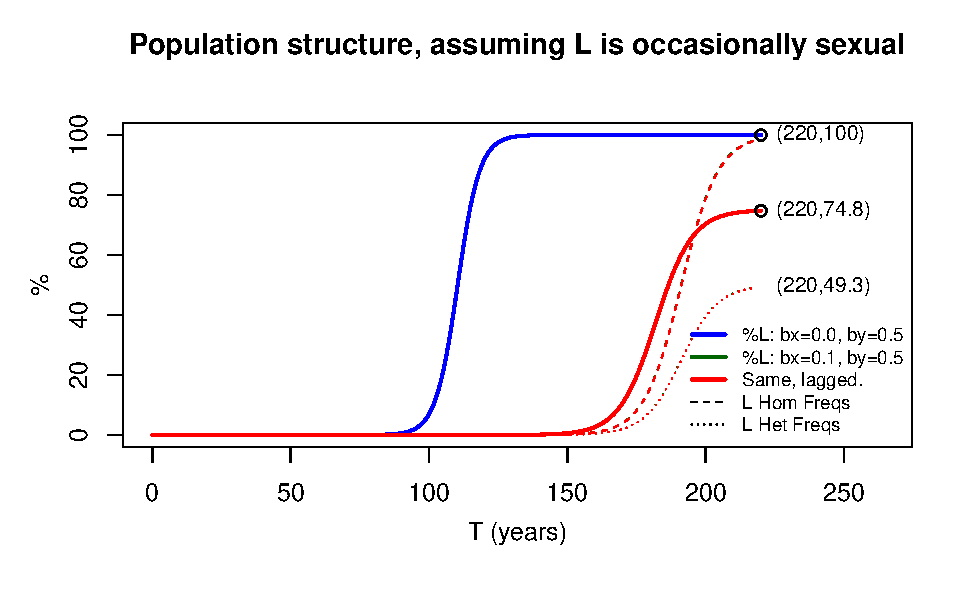
\includegraphics[width=\maxwidth]{asex-figs-knitr/unnamed-chunk-19-1} 

}



\end{knitrout}

Seemingly, not much change; invisible on this scale.

This reproduces the key features of the earlier figure -- assuming non-zero meiotic rate (non-blue
curves), L rises to a stable fraction of the population $< 100\%$, and all heterozygous positions in
L rise to 50\% allele frequency within the non-L population.  Not shown, but still true --
homozygous positions in L rise to 100\% in non-L.  I.e., pre-existing non-L alleles are totally
washed out of the population.

\subsection{Model 4: Simple Mendelian Recessive}
\label{sec:smr}

To recap: Under the simple assumptions modeled above, (Model 1) an obligate asexual genotype will
sweep the world, whereas (Model 2) a facultative sexual genotype with reduced frequency of meiosis
will sweep to a large fraction of the population, but stably coexist with its sexually derived
offspring.  Our observational data is plausibly consistent with a transient state\footnote
{ 
  Continued existence of the H isolates also may depend on factors completely 
  outside the scope of the models considered here.  For example, geographical isolation, 
  esp. of the Italian isolate, may be at play, as may increased fitness to local 
  environmental conditions.
}
of (M1), and, at first blush, with (M2), although that doesn't hold up vs the more detailed model
(M2prime).  I claim that an additional \textit{very plausible} genetic assumption is enough to
render the ``facultative sexual'' model even less likely.

What might cause an increase in the average time between meiotic events?  One model, perhaps the
simplest, is that the increased interval is a simple Mendelian recessive trait---some single gene
involved in meiosis has acquired a non-wildtype allele that, when homozygous, reduces the frequency
of meiosis.  I.e., assume that L is homozygous for the recessive allele of this gene, call it ``ss''
(``SlowSex'').  (``Recessive'' as opposed to dominant or additive is the more conservative choice I
believe; either of these alternatives would sweep more rapidly, making the intermediate state less
likely to be observed; considered briefly below as well.)

As intuition for how this would affect thaps evolution, note that the L-genotype, sexual or not, has
a growth advantage over both the wildtype and over heterozygotes.  But if L remains sexual, it would
continuously inject the ss allele into the non-L gene pool.  (We have previously argued that all
sexual offspring of L will have a recognizably non-L genotype.)  As seen in the two models above, L
rises exponentially in frequency.  When its frequency is small, its contribution to the non-L gene
pool is negligible, but after L attains a substantial representation, the proportion of ss injected
into the non-L population becomes significant, after which \textit{non-L homozygotes} will emerge,
and they will have at least the same growth advantage as L has over wildtype.  Thus, the ss allele
will increase in frequency \textit{among non-L genotypes}, eventually dominating the population.
Furthermore, the L genotype is at a competitive disadvantage when compared to homozygous non-L,
since sexual offspring of L genotypes are never of that genotype, whereas sexual offspring of
homozygous non-L sometimes retain homozygosity. Said more simply, the ``ss'' allele, while
recessive, is evolutionarily favored, at least in the short term, and will sweep to fixation, once
given a kick-start by creation of the homozygous L-genotype.  It's surprisingly easy.

The simulations below support this intuition, with the ss allele rapidly fixing in the population,
and with the additional nuance that the L genotype is only ephemerally dominant in the population,
and decreasingly so as the gap between $b_x$ and $b_y$ shrinks.  Consequently, our observed data
with 5 of 7 samples matching the L genotype seems more likely to reflect the ``obligate asexual''
model (see footnote 1 again) than the ``facultative sexual, Mendelian recessive, sampled at just the
right time'' model.  However, I admit that the data are not conclusive.

\begin{knitrout}\footnotesize
\definecolor{shadecolor}{rgb}{0.969, 0.969, 0.969}\color{fgcolor}\begin{kframe}
\begin{alltt}
\hlcom{# grow4 simulates 'yrs' years of growth in the 4-component model where L's lower meiotic}
\hlcom{# rate is assumed to be driven by presence of homozygous recessive form of some one gene. }
\hlcom{# Gene flow from L to non-L is tracked, separately accounting for non-L types having 0, 1}
\hlcom{# or 2 copies of the recessive allele. 0 and 1 copy cells are assumed to have b_y meioses}
\hlcom{# per year; 2 copies (incl L) have b_x.  All have equal mitotic rates.}
\hlstd{grow4} \hlkwb{<-} \hlkwa{function}\hlstd{(}\hlkwc{yrs}\hlstd{,} \hlkwc{a}\hlstd{=}\hlnum{180}\hlstd{,} \hlkwc{bx}\hlstd{=}\hlnum{0.2}\hlstd{,} \hlkwc{by}\hlstd{=}\hlnum{0.5}\hlstd{,} \hlkwc{k}\hlstd{=}\hlnum{2}\hlstd{,} \hlkwc{f}\hlstd{=}\hlnum{2}\hlstd{,} \hlkwc{p0}\hlstd{=}\hlnum{1e-12}\hlstd{,} \hlkwc{recessive}\hlstd{=}\hlnum{TRUE}\hlstd{)\{}
  \hlstd{n} \hlkwb{<-} \hlkwd{round}\hlstd{(yrs}\hlopt{*}\hlstd{a}\hlopt{/}\hlstd{k)} \hlcom{# number of epochs to simulate}
  \hlstd{x} \hlkwb{<-} \hlkwd{numeric}\hlstd{(n)}     \hlcom{# proportion in L}
  \hlstd{y0}\hlkwb{<-} \hlkwd{numeric}\hlstd{(n)}     \hlcom{# proportion non-L with 0 copies}
  \hlstd{y1}\hlkwb{<-} \hlkwd{numeric}\hlstd{(n)}     \hlcom{# proportion non-L 1 copy}
  \hlstd{y2}\hlkwb{<-} \hlkwd{numeric}\hlstd{(n)}     \hlcom{# proportion non-L 2 copies}
  \hlstd{betax} \hlkwb{<-} \hlstd{bx}\hlopt{/}\hlstd{(a}\hlopt{/}\hlstd{k)}   \hlcom{# meioses per epoch in L and y2}
  \hlstd{betay} \hlkwb{<-} \hlstd{by}\hlopt{/}\hlstd{(a}\hlopt{/}\hlstd{k)}   \hlcom{# meioses per epoch in non-L y0, y1}
  \hlstd{x[}\hlnum{1}\hlstd{]}  \hlkwb{<-} \hlstd{p0}         \hlcom{# initial proportion in L }
  \hlstd{y2[}\hlnum{1}\hlstd{]} \hlkwb{<-} \hlnum{0}
  \hlstd{y1[}\hlnum{1}\hlstd{]} \hlkwb{<-} \hlnum{0}          \hlcom{# p0 is also reasonable here, but <- 0 is conservative}
  \hlstd{y0[}\hlnum{1}\hlstd{]} \hlkwb{<-} \hlnum{1}\hlopt{-}\hlstd{x[}\hlnum{1}\hlstd{]}
  \hlkwa{for}\hlstd{(i} \hlkwa{in} \hlnum{2}\hlopt{:}\hlstd{n)\{}
    \hlcom{# total meiotic fraction}
    \hlstd{z} \hlkwb{<-} \hlstd{(x[i}\hlopt{-}\hlnum{1}\hlstd{]}\hlopt{+}\hlstd{y2[i}\hlopt{-}\hlnum{1}\hlstd{])}\hlopt{*}\hlstd{betax} \hlopt{+} \hlstd{(y1[i}\hlopt{-}\hlnum{1}\hlstd{]}\hlopt{+}\hlstd{y0[i}\hlopt{-}\hlnum{1}\hlstd{])}\hlopt{*}\hlstd{betay}
    \hlcom{# fraction of recessive chromosomes among meiotics}
    \hlstd{p} \hlkwb{<-} \hlstd{(}\hlnum{2}\hlopt{*}\hlstd{(x[i}\hlopt{-}\hlnum{1}\hlstd{]}\hlopt{+}\hlstd{y2[i}\hlopt{-}\hlnum{1}\hlstd{])}\hlopt{*}\hlstd{betax} \hlopt{+} \hlnum{1}\hlopt{*}\hlstd{y1[i}\hlopt{-}\hlnum{1}\hlstd{]}\hlopt{*}\hlstd{betay)}\hlopt{/}\hlstd{(}\hlnum{2}\hlopt{*}\hlstd{z)}
    \hlstd{q} \hlkwb{<-} \hlnum{1}\hlopt{-}\hlstd{p}
    \hlkwa{if}\hlstd{(i}\hlopt{<}\hlnum{0}\hlstd{)\{} \hlcom{# debug}
      \hlkwd{cat}\hlstd{(}\hlstr{'yrs='}\hlstd{,yrs,}\hlstr{'a='}\hlstd{,a,}\hlstr{'k='}\hlstd{,k,}\hlstr{'n='}\hlstd{,n,}\hlstr{'i='}\hlstd{,i,}\hlstr{'betax='}\hlstd{,betax,}\hlstr{'betay='}\hlstd{,betay,}
          \hlstr{'z='}\hlstd{,z,}\hlstr{'p='}\hlstd{,p,} \hlstr{'1-q='}\hlstd{,}\hlnum{1}\hlopt{-}\hlstd{q,}\hlstr{'x[i-1]='}\hlstd{,x[i}\hlopt{-}\hlnum{1}\hlstd{],}\hlstr{'\textbackslash{}n'}\hlstd{)}
    \hlstd{\}}
    \hlcom{# Despite all the comments about "recessive", I also wanted to see what happens if the}
    \hlcom{# trait is dominant, which just involves changing the "beta" coefficient in the y1}
    \hlcom{# calcuation below.}
    \hlkwa{if}\hlstd{(recessive)\{}
      \hlstd{beta1} \hlkwb{<-} \hlstd{betay}
    \hlstd{\}} \hlkwa{else} \hlstd{\{}
      \hlstd{beta1} \hlkwb{<-} \hlstd{betax}
    \hlstd{\}}
    \hlcom{# new population fractions, assuming random mating}
    \hlstd{x[i]}  \hlkwb{<-}  \hlstd{x[i}\hlopt{-}\hlnum{1}\hlstd{]}\hlopt{*}\hlstd{(}\hlnum{1}\hlopt{-}\hlstd{betax)}\hlopt{*}\hlnum{2}\hlopt{^}\hlstd{k}
    \hlstd{y2[i]} \hlkwb{<-} \hlstd{y2[i}\hlopt{-}\hlnum{1}\hlstd{]}\hlopt{*}\hlstd{(}\hlnum{1}\hlopt{-}\hlstd{betax)}\hlopt{*}\hlnum{2}\hlopt{^}\hlstd{k} \hlopt{+}   \hlstd{p}\hlopt{^}\hlnum{2} \hlopt{*} \hlstd{z} \hlopt{*} \hlstd{f} \hlcom{# \textbackslash{}}
    \hlstd{y1[i]} \hlkwb{<-} \hlstd{y1[i}\hlopt{-}\hlnum{1}\hlstd{]}\hlopt{*}\hlstd{(}\hlnum{1}\hlopt{-}\hlstd{beta1)}\hlopt{*}\hlnum{2}\hlopt{^}\hlstd{k} \hlopt{+} \hlnum{2}\hlopt{*}\hlstd{p}\hlopt{*}\hlstd{q} \hlopt{*} \hlstd{z} \hlopt{*} \hlstd{f} \hlcom{#  \}-- Hardy Weinberg proportions }
    \hlstd{y0[i]} \hlkwb{<-} \hlstd{y0[i}\hlopt{-}\hlnum{1}\hlstd{]}\hlopt{*}\hlstd{(}\hlnum{1}\hlopt{-}\hlstd{betay)}\hlopt{*}\hlnum{2}\hlopt{^}\hlstd{k} \hlopt{+}   \hlstd{q}\hlopt{^}\hlnum{2} \hlopt{*} \hlstd{z} \hlopt{*} \hlstd{f} \hlcom{# /}
    \hlcom{# re-normalize:}
    \hlstd{w} \hlkwb{<-} \hlstd{x[i]}\hlopt{+}\hlstd{y2[i]}\hlopt{+}\hlstd{y1[i]}\hlopt{+}\hlstd{y0[i]}
    \hlstd{x[i]}  \hlkwb{<-}  \hlstd{x[i]}\hlopt{/}\hlstd{w}
    \hlstd{y2[i]} \hlkwb{<-} \hlstd{y2[i]}\hlopt{/}\hlstd{w}
    \hlstd{y1[i]} \hlkwb{<-} \hlstd{y1[i]}\hlopt{/}\hlstd{w}
   \hlcom{#y0[i] <- y0[i]/w}
    \hlstd{y0[i]} \hlkwb{<-} \hlnum{1.0}\hlopt{-}\hlstd{x[i]}\hlopt{-}\hlstd{y2[i]}\hlopt{-}\hlstd{y1[i]} \hlcom{# slightly more robust to roundoff errs, I think}
  \hlstd{\}}
  \hlstd{t} \hlkwb{<-} \hlstd{((}\hlnum{1}\hlopt{:}\hlstd{n)}\hlopt{-}\hlnum{1}\hlstd{)}\hlopt{/}\hlstd{a}\hlopt{*}\hlstd{k} \hlcom{# rescale epoch numbers to years}
  \hlkwd{return}\hlstd{(}\hlkwd{list}\hlstd{(}\hlkwc{x}\hlstd{=x,}\hlkwc{y2}\hlstd{=y2,}\hlkwc{y1}\hlstd{=y1,}\hlkwc{y0}\hlstd{=y0,}\hlkwc{t}\hlstd{=t,}\hlkwc{yrs}\hlstd{=yrs,}\hlkwc{bx}\hlstd{=bx,}\hlkwc{by}\hlstd{=by,}\hlkwc{a}\hlstd{=a,}\hlkwc{k}\hlstd{=k,}\hlkwc{f}\hlstd{=f))}
\hlstd{\}}

\hlcom{# plot4 plots a growth series g (as returned by grow4). Plots all 4 subpopulations.}
\hlstd{plot4} \hlkwb{<-} \hlkwa{function}\hlstd{(}\hlkwc{g}\hlstd{,} \hlkwc{main.sub.label}\hlstd{=}\hlstr{''}\hlstd{,} \hlkwc{where}\hlstd{=}\hlstr{'topright'}\hlstd{,} \hlkwc{showLMax}\hlstd{=}\hlnum{TRUE}\hlstd{,} \hlkwc{recessive}\hlstd{=}\hlnum{TRUE}\hlstd{,} \hlkwc{no.main}\hlstd{=}\hlnum{FALSE}\hlstd{)\{}
  \hlcom{# Set up plot axes }
  \hlstd{main.label} \hlkwb{<-} \hlkwd{paste}\hlstd{(}\hlstr{'Mendelian'}\hlstd{,} \hlkwd{ifelse}\hlstd{(recessive,} \hlstr{'recessive'}\hlstd{,} \hlstr{'dominant'}\hlstd{),} \hlstr{'model'}\hlstd{)}
  \hlkwa{if}\hlstd{(main.sub.label} \hlopt{!=} \hlstr{''}\hlstd{)\{}
    \hlstd{main.label} \hlkwb{<-} \hlkwd{paste}\hlstd{(main.label, main.sub.label,} \hlkwc{sep}\hlstd{=}\hlstr{', '}\hlstd{)}
  \hlstd{\}}
  \hlkwa{if}\hlstd{(no.main)\{}
    \hlcom{# for supp fig, no main title & tighter margins}
    \hlstd{main.label} \hlkwb{<-} \hlnum{NA}
    \hlstd{opar} \hlkwb{<-} \hlkwd{par}\hlstd{(}\hlkwc{no.readonly}\hlstd{=T,} \hlkwc{mar}\hlstd{=}\hlkwd{c}\hlstd{(}\hlnum{3.5}\hlstd{,}\hlnum{3.5}\hlstd{,}\hlnum{2}\hlstd{,}\hlnum{1}\hlstd{)}\hlopt{+}\hlnum{0.1}\hlstd{);} \hlkwd{on.exit}\hlstd{(}\hlkwd{par}\hlstd{(opar))}
    \hlstd{\}}
  \hlkwd{plot}\hlstd{(}\hlkwa{NULL}\hlstd{,}\hlkwc{type}\hlstd{=}\hlstr{'n'}\hlstd{,} \hlkwc{xlim}\hlstd{=}\hlkwd{c}\hlstd{(}\hlnum{0}\hlstd{,}\hlnum{1.2}\hlopt{*}\hlstd{g}\hlopt{$}\hlstd{yrs),} \hlkwc{ylim}\hlstd{=}\hlkwd{c}\hlstd{(}\hlnum{0}\hlstd{,}\hlnum{100}\hlstd{),} \hlkwc{main}\hlstd{=}\hlnum{NA}\hlstd{,}\hlkwc{xlab}\hlstd{=}\hlnum{NA}\hlstd{,}\hlkwc{ylab}\hlstd{=}\hlnum{NA}\hlstd{)}
  \hlkwd{title}\hlstd{(}\hlkwc{xlab}\hlstd{=}\hlstr{'T (years)'}\hlstd{,} \hlkwc{ylab}\hlstd{=}\hlstr{'%'}\hlstd{,} \hlkwc{main}\hlstd{=main.label,} \hlkwc{line}\hlstd{=}\hlnum{2.3}\hlstd{)}
  \hlstd{n} \hlkwb{<-} \hlkwd{length}\hlstd{(g}\hlopt{$}\hlstd{t)}
  \hlkwa{if}\hlstd{(n} \hlopt{<} \hlnum{2048}\hlstd{)\{}
    \hlkwd{lines}\hlstd{(g}\hlopt{$}\hlstd{t,  g}\hlopt{$}\hlstd{x}\hlopt{*}\hlnum{100}\hlstd{,} \hlkwc{lwd}\hlstd{=}\hlnum{2}\hlstd{,} \hlkwc{col}\hlstd{=}\hlstr{'red'}\hlstd{)}
    \hlkwd{lines}\hlstd{(g}\hlopt{$}\hlstd{t, g}\hlopt{$}\hlstd{y2}\hlopt{*}\hlnum{100}\hlstd{,} \hlkwc{lwd}\hlstd{=}\hlnum{2}\hlstd{,} \hlkwc{col}\hlstd{=}\hlstr{'orange'}\hlstd{)}
    \hlkwd{lines}\hlstd{(g}\hlopt{$}\hlstd{t, g}\hlopt{$}\hlstd{y1}\hlopt{*}\hlnum{100}\hlstd{,} \hlkwc{lwd}\hlstd{=}\hlnum{2}\hlstd{,} \hlkwc{col}\hlstd{=}\hlstr{'darkgreen'}\hlstd{)}
    \hlkwd{lines}\hlstd{(g}\hlopt{$}\hlstd{t, g}\hlopt{$}\hlstd{y0}\hlopt{*}\hlnum{100}\hlstd{,} \hlkwc{lwd}\hlstd{=}\hlnum{2}\hlstd{,} \hlkwc{col}\hlstd{=}\hlstr{'blue'}\hlstd{)}
    \hlkwa{if}\hlstd{(}\hlopt{!}\hlstd{recessive)\{}
      \hlkwd{lines}\hlstd{(g}\hlopt{$}\hlstd{t,(g}\hlopt{$}\hlstd{y1}\hlopt{+}\hlstd{g}\hlopt{$}\hlstd{y2)}\hlopt{*}\hlnum{100}\hlstd{,} \hlkwc{lwd}\hlstd{=}\hlnum{1}\hlstd{,} \hlkwc{col}\hlstd{=}\hlstr{'orange'}\hlstd{,} \hlkwc{lty}\hlstd{=}\hlstr{'dashed'}\hlstd{)}
    \hlstd{\}}
  \hlstd{\}} \hlkwa{else} \hlstd{\{}
    \hlcom{# For long series, sufficient, and much faster, to plot a subsequence}
    \hlstd{k} \hlkwb{<-} \hlkwd{floor}\hlstd{(n}\hlopt{/}\hlnum{1024}\hlstd{)}
    \hlstd{s} \hlkwb{<-} \hlkwd{seq}\hlstd{(}\hlkwc{from}\hlstd{=}\hlnum{1}\hlstd{,}\hlkwc{by}\hlstd{=k,}\hlkwc{to}\hlstd{=n)}
    \hlkwd{lines}\hlstd{(g}\hlopt{$}\hlstd{t[s],  g}\hlopt{$}\hlstd{x[s]}\hlopt{*}\hlnum{100}\hlstd{,} \hlkwc{lwd}\hlstd{=}\hlnum{2}\hlstd{,} \hlkwc{col}\hlstd{=}\hlstr{'red'}\hlstd{)}
    \hlkwd{lines}\hlstd{(g}\hlopt{$}\hlstd{t[s], g}\hlopt{$}\hlstd{y2[s]}\hlopt{*}\hlnum{100}\hlstd{,} \hlkwc{lwd}\hlstd{=}\hlnum{2}\hlstd{,} \hlkwc{col}\hlstd{=}\hlstr{'orange'}\hlstd{)}
    \hlkwd{lines}\hlstd{(g}\hlopt{$}\hlstd{t[s], g}\hlopt{$}\hlstd{y1[s]}\hlopt{*}\hlnum{100}\hlstd{,} \hlkwc{lwd}\hlstd{=}\hlnum{2}\hlstd{,} \hlkwc{col}\hlstd{=}\hlstr{'darkgreen'}\hlstd{)}
    \hlkwd{lines}\hlstd{(g}\hlopt{$}\hlstd{t[s], g}\hlopt{$}\hlstd{y0[s]}\hlopt{*}\hlnum{100}\hlstd{,} \hlkwc{lwd}\hlstd{=}\hlnum{2}\hlstd{,} \hlkwc{col}\hlstd{=}\hlstr{'blue'}\hlstd{)}
    \hlkwa{if}\hlstd{(}\hlopt{!}\hlstd{recessive)\{}
      \hlkwd{lines}\hlstd{(g}\hlopt{$}\hlstd{t[s],(g}\hlopt{$}\hlstd{y1[s]}\hlopt{+}\hlstd{g}\hlopt{$}\hlstd{y2[s])}\hlopt{*}\hlnum{100}\hlstd{,} \hlkwc{lwd}\hlstd{=}\hlnum{1}\hlstd{,} \hlkwc{col}\hlstd{=}\hlstr{'orange'}\hlstd{,} \hlkwc{lty}\hlstd{=}\hlstr{'dashed'}\hlstd{)}
    \hlstd{\}}
  \hlstd{\}}
  \hlcom{# print((g$y1[n]+g$y2[n])*100)}
  \hlkwd{legend}\hlstd{(where,} \hlkwc{lwd}\hlstd{=}\hlnum{2}\hlstd{,} \hlkwc{bty}\hlstd{=}\hlstr{'n'}\hlstd{,} \hlkwc{inset}\hlstd{=}\hlkwd{c}\hlstd{(}\hlnum{0}\hlstd{,}\hlnum{0.1}\hlstd{),}
         \hlkwc{title}\hlstd{=}\hlkwd{paste}\hlstd{(}\hlstr{'a='}\hlstd{, g}\hlopt{$}\hlstd{a,} \hlstr{' bx='}\hlstd{, g}\hlopt{$}\hlstd{bx,}\hlstr{' by='}\hlstd{, g}\hlopt{$}\hlstd{by,} \hlstr{' k='}\hlstd{, g}\hlopt{$}\hlstd{k,}\hlstr{' f='}\hlstd{, g}\hlopt{$}\hlstd{f,} \hlkwc{sep}\hlstd{=}\hlstr{''}\hlstd{),}
         \hlkwc{legend}\hlstd{=}\hlkwd{c}\hlstd{(}\hlstr{'x  (L genotype)'}\hlstd{,}
                  \hlstr{'y2 (non-L, hom "slow sex")'}\hlstd{,}
                  \hlstr{'y1 (non-L, het)'}\hlstd{,}
                  \hlstr{'y0 (non-L, hom wildtype)'}\hlstd{),}
         \hlkwc{col}\hlstd{=}   \hlkwd{c}\hlstd{(}\hlstr{'red'}\hlstd{,} \hlstr{'orange'}\hlstd{,} \hlstr{'darkgreen'}\hlstd{,} \hlstr{'blue'}\hlstd{))}
  \hlkwa{if}\hlstd{(showLMax)\{}
    \hlcom{# annotate the max x point}
    \hlstd{i} \hlkwb{<-} \hlkwd{which.max}\hlstd{(g}\hlopt{$}\hlstd{x)}
    \hlkwd{points}\hlstd{(g}\hlopt{$}\hlstd{t[i],g}\hlopt{$}\hlstd{x[i]}\hlopt{*}\hlnum{100}\hlstd{,}\hlkwc{col}\hlstd{=}\hlstr{'red'}\hlstd{)}
    \hlkwd{text}\hlstd{(g}\hlopt{$}\hlstd{t[i], g}\hlopt{$}\hlstd{x[i]}\hlopt{*}\hlnum{100}\hlstd{,}
         \hlkwd{paste}\hlstd{(}\hlstr{'('}\hlstd{,} \hlkwd{round}\hlstd{(g}\hlopt{$}\hlstd{t[i]),} \hlstr{', '}\hlstd{,} \hlkwd{round}\hlstd{(g}\hlopt{$}\hlstd{x[i]}\hlopt{*}\hlnum{100}\hlstd{,}\hlnum{1}\hlstd{),}\hlstr{'%)'}\hlstd{,} \hlkwc{sep}\hlstd{=}\hlstr{''}\hlstd{),}
         \hlkwc{pos}\hlstd{=}\hlnum{4}\hlstd{,} \hlkwc{col}\hlstd{=}\hlstr{'red'}\hlstd{)}
    \hlcom{# and if x exceeds 50%, show where, & for how long}
    \hlstd{maj} \hlkwb{<-} \hlkwd{which}\hlstd{(g}\hlopt{$}\hlstd{x}\hlopt{>=}\hlnum{0.5}\hlstd{)}
    \hlstd{majn} \hlkwb{<-} \hlkwd{length}\hlstd{(maj)}
    \hlkwa{if}\hlstd{(majn} \hlopt{>} \hlnum{0}\hlstd{)\{}
      \hlstd{majt} \hlkwb{<-} \hlstd{g}\hlopt{$}\hlstd{t[maj[}\hlkwd{c}\hlstd{(}\hlnum{1}\hlstd{,majn)]]}        \hlcom{# 1st, last times}
      \hlkwd{lines}\hlstd{(majt,}\hlkwd{c}\hlstd{(}\hlnum{50}\hlstd{,}\hlnum{50}\hlstd{),}\hlkwc{lwd}\hlstd{=}\hlnum{0.5}\hlstd{,}\hlkwc{lty}\hlstd{=}\hlnum{2}\hlstd{)} \hlcom{# draw a line there & say how many yrs}
      \hlkwd{text}\hlstd{(majt[}\hlnum{2}\hlstd{],} \hlnum{50}\hlstd{,} \hlkwd{paste}\hlstd{(}\hlkwd{round}\hlstd{(majt[}\hlnum{2}\hlstd{]}\hlopt{-}\hlstd{majt[}\hlnum{1}\hlstd{]),}\hlstr{'yrs'}\hlstd{),}\hlkwc{pos}\hlstd{=}\hlnum{4}\hlstd{,} \hlkwc{cex}\hlstd{=}\hlnum{.7}\hlstd{,}\hlkwc{col}\hlstd{=}\hlstr{'red'}\hlstd{)}
    \hlstd{\}}
  \hlstd{\}}
\hlstd{\}}
\hlcom{# plot an example}
\hlstd{growex4} \hlkwb{<-} \hlkwa{function}\hlstd{(}\hlkwc{yrs}\hlstd{=}\hlnum{600}\hlstd{,} \hlkwc{a}\hlstd{=}\hlnum{180}\hlstd{,} \hlkwc{bx}\hlstd{=}\hlnum{0.2}\hlstd{,} \hlkwc{by}\hlstd{=}\hlnum{0.5}\hlstd{,} \hlkwc{k}\hlstd{=}\hlnum{2}\hlstd{,} \hlkwc{f}\hlstd{=}\hlnum{2}\hlstd{,} \hlkwc{p0}\hlstd{=}\hlnum{1e-12}\hlstd{,} \hlkwc{where}\hlstd{=}\hlstr{'topright'}\hlstd{,}
                    \hlkwc{verbose}\hlstd{=}\hlnum{FALSE}\hlstd{,} \hlkwc{recessive}\hlstd{=}\hlnum{TRUE}\hlstd{,} \hlkwc{main.sub.label}\hlstd{=}\hlstr{''}\hlstd{,} \hlkwc{no.main}\hlstd{=}\hlnum{FALSE}\hlstd{)\{}
  \hlstd{ex} \hlkwb{<-} \hlkwd{grow4}\hlstd{(yrs, a, bx, by, k, f, p0, recessive)}
  \hlkwd{plot4}\hlstd{(ex, where,} \hlkwc{recessive}\hlstd{=recessive,} \hlkwc{main.sub.label}\hlstd{=main.sub.label,} \hlkwc{no.main}\hlstd{=no.main)}
  \hlkwa{if}\hlstd{(verbose)\{}
    \hlstd{n} \hlkwb{<-}\hlkwd{length}\hlstd{(ex}\hlopt{$}\hlstd{x)}
    \hlkwd{print}\hlstd{(}\hlkwd{rbind}\hlstd{(}
      \hlstr{'x-p0'}\hlstd{=ex}\hlopt{$}\hlstd{x[}\hlkwd{c}\hlstd{(}\hlnum{1}\hlopt{:}\hlnum{5}\hlstd{,n)]}\hlopt{-}\hlstd{p0,}
      \hlkwc{y2}  \hlstd{=ex}\hlopt{$}\hlstd{y2[}\hlkwd{c}\hlstd{(}\hlnum{1}\hlopt{:}\hlnum{5}\hlstd{,n)],}
      \hlkwc{y1}  \hlstd{=ex}\hlopt{$}\hlstd{y1[}\hlkwd{c}\hlstd{(}\hlnum{1}\hlopt{:}\hlnum{5}\hlstd{,n)],}
      \hlstr{'1-y0'}\hlstd{=}\hlnum{1}\hlopt{-}\hlstd{ex}\hlopt{$}\hlstd{y0[}\hlkwd{c}\hlstd{(}\hlnum{1}\hlopt{:}\hlnum{5}\hlstd{,n)]}
    \hlstd{))}
    \hlcom{#print(1-ex$y0[1:5]-ex$x[1:5]-ex$y1[1:5]-ex$y2[1:5])}
    \hlcom{#print(summary(1-ex$y0-ex$x-ex$y1-ex$y2)) ##$}
  \hlstd{\}}
\hlstd{\}}
\end{alltt}
\end{kframe}
\end{knitrout}

The examples shown below all use the same parameters $a=180, b_y=0.5, k=2, f=2, p_0=10^{-12}$ as in
the earlier sections; they differ in that they model a hypothetical Mendelian recessive allele
which, when homozygous, lowers the meiotic rate to $b_x=0.05, \ldots, 0.24$, (vs $b_y=0.5$ for
heterozygotes and for homozygous wild type).  In all, the wild-type remains dominant for a few
centuries, then crashes rapidly as the L-genotype starts reaching significant levels, but the
L-genotype's rise is quicky reversed as ss-homozygous non-L genotypes out-compete and/or interbreed
with it.  The L-genotype exceeds 50\% of the population only in the first simulation, and only
briefly ($\approx30$ years); note that this simulation assumes an average of 20 years between
meioses, ten-fold less frequent than the default model of once every 2 years.

\begin{knitrout}\footnotesize
\definecolor{shadecolor}{rgb}{0.969, 0.969, 0.969}\color{fgcolor}\begin{kframe}
\begin{alltt}
\hlkwd{pdf}\hlstd{(}\hlkwd{fpath}\hlstd{(}\hlstr{'Fig-S10B'}\hlstd{),} \hlkwc{width}\hlstd{=}\hlnum{6.5}\hlstd{,} \hlkwc{height}\hlstd{=}\hlnum{4}\hlstd{)}
\hlkwd{growex4}\hlstd{(}\hlkwc{yrs}\hlstd{=}\hlnum{700}\hlstd{,}\hlkwc{bx}\hlstd{=}\hlnum{0.05}\hlstd{,} \hlkwc{main.sub.label}\hlstd{=}\hlstr{'bx=0.05'}\hlstd{,} \hlkwc{no.main}\hlstd{=}\hlnum{TRUE}\hlstd{)}
\hlkwd{text}\hlstd{(}\hlnum{0}\hlstd{,}\hlnum{90}\hlstd{,}\hlstr{'B'}\hlstd{,}\hlkwc{cex}\hlstd{=}\hlnum{1.5}\hlstd{)}
\hlstd{no.chatter} \hlkwb{<-} \hlkwd{dev.off}\hlstd{()}
\end{alltt}
\end{kframe}
\end{knitrout}

\dofig{asex-figs-mine/Fig-S10B.pdf}{(Fig-S10B): Mendelian recessive model, bx=0.05}{fig:S10B}

Raising $b_x$ from 0.05 to 0.24 (the next three plots) delays the transition and lowers the extent
of L expansion, but otherwise recapitulates the phenomena seen above.

\begin{knitrout}\footnotesize
\definecolor{shadecolor}{rgb}{0.969, 0.969, 0.969}\color{fgcolor}\begin{kframe}
\begin{alltt}
\hlkwd{growex4}\hlstd{(}\hlkwc{bx}\hlstd{=}\hlnum{0.1}\hlstd{,} \hlkwc{main.sub.label}\hlstd{=}\hlstr{'bx=0.1'}\hlstd{)}
\end{alltt}
\end{kframe}

{\centering \includegraphics[width=\maxwidth]{asex-figs-knitr/unnamed-chunk-21-1} 

}



\end{knitrout}

\begin{knitrout}\footnotesize
\definecolor{shadecolor}{rgb}{0.969, 0.969, 0.969}\color{fgcolor}\begin{kframe}
\begin{alltt}
\hlkwd{growex4}\hlstd{(}\hlkwc{bx}\hlstd{=}\hlnum{0.2}\hlstd{,} \hlkwc{main.sub.label}\hlstd{=}\hlstr{'bx=0.2'}\hlstd{,}\hlkwc{where}\hlstd{=}\hlstr{'bottomleft'}\hlstd{)}
\end{alltt}
\end{kframe}

{\centering \includegraphics[width=\maxwidth]{asex-figs-knitr/unnamed-chunk-22-1} 

}



\end{knitrout}

\begin{knitrout}\footnotesize
\definecolor{shadecolor}{rgb}{0.969, 0.969, 0.969}\color{fgcolor}\begin{kframe}
\begin{alltt}
\hlkwd{growex4}\hlstd{(}\hlkwc{bx}\hlstd{=}\hlnum{0.24}\hlstd{,} \hlkwc{main.sub.label}\hlstd{=}\hlstr{'bx=0.24'}\hlstd{,} \hlkwc{where}\hlstd{=}\hlstr{'bottomleft'}\hlstd{,}\hlkwc{yrs}\hlstd{=}\hlnum{2500}\hlstd{)}
\end{alltt}
\end{kframe}

{\centering \includegraphics[width=\maxwidth]{asex-figs-knitr/unnamed-chunk-23-1} 

}



\end{knitrout}

There is, however, a qualitative change in character as $b_x$ increases from 0.24 to 0.25.  As in
the examples above, $b_x<b_y$ implies a growth advantage for the homozygous recessive genotypes
since they undergo (slow) meiosis less frequently.  However, for any $b_x>0$, this growth advantage
is at least partially offset by meiotic disruption of homozygosity.  E.g., when $b_x=0.25$, one
quarter of the homozygous recessive population undergoes meiosis every year, mostly mating with
cells \textit{not} carrying the ss allele (until its allele frequency rises).  At $b_x=0.25$, these
effects apparently balance, preventing the ss allele frequency from growing appreciably, even over a
100 thousand year span:

\begin{knitrout}\footnotesize
\definecolor{shadecolor}{rgb}{0.969, 0.969, 0.969}\color{fgcolor}\begin{kframe}
\begin{alltt}
\hlkwd{growex4}\hlstd{(}\hlkwc{bx}\hlstd{=}\hlnum{0.25}\hlstd{,} \hlkwc{main.sub.label}\hlstd{=}\hlstr{'bx=0.25'}\hlstd{,} \hlkwc{where}\hlstd{=}\hlstr{'bottomleft'}\hlstd{,}\hlkwc{yrs}\hlstd{=}\hlkwd{ifelse}\hlstd{(QUICKLY,}\hlnum{100}\hlstd{,}\hlnum{100000}\hlstd{),}\hlkwc{verbose} \hlstd{=} \hlnum{TRUE}\hlstd{)}
\end{alltt}
\begin{verbatim}
#              [,1]          [,2]          [,3]          [,4]          [,5]          [,6]
# x-p0 0.000000e+00 -1.413639e-27 -2.827277e-27 -4.240916e-27 -5.654555e-27 -1.783971e-20
# y2   0.000000e+00  6.963788e-28  1.396643e-27  2.100802e-27  2.808868e-27  1.869332e-12
# y1   0.000000e+00  2.785515e-15  5.571031e-15  8.356546e-15  1.114206e-14  3.513800e-08
# 1-y0 9.999779e-13  1.002753e-12  1.005529e-12  1.008305e-12  1.011080e-12  3.514087e-08
\end{verbatim}
\end{kframe}

{\centering \includegraphics[width=\maxwidth]{asex-figs-knitr/unnamed-chunk-24-1} 

}



\end{knitrout}

If we instead assume that slow sex is a \textit{dominant} trait then, in comparison to the first
parameterization plotted in this section, dominance speeds the transition by about 50 years, and
suppresses growth of the L genotype, but does not result in fixation of the ss allele, as seen in
the plot below.  Instead, the wild type persists at a low but stable level.  Presumably because
heterozygotes also get the growth advantage, hets persist in the population, and HWE then yields 
a few homozygous wild-type cells.  [[Or maybe there's a bug in my code...]]  (Out of laziness, 
the plot below is somewhat mislabeled, but the key new feature is the dashed orange line, which 
records the percentage of the population with 1 \textit{or} 2 copies of the ss allele.  Key 
point is that it does \textit{not} reach 100\%.)

\begin{knitrout}\footnotesize
\definecolor{shadecolor}{rgb}{0.969, 0.969, 0.969}\color{fgcolor}\begin{kframe}
\begin{alltt}
\hlkwd{growex4}\hlstd{(}\hlkwc{bx}\hlstd{=}\hlnum{0.05}\hlstd{,}\hlkwc{recessive}\hlstd{=}\hlnum{FALSE}\hlstd{)}
\end{alltt}
\end{kframe}

{\centering \includegraphics[width=\maxwidth]{asex-figs-knitr/unnamed-chunk-25-1} 

}



\end{knitrout}

I expect an additive model (i.e., the heterozygote phenotype is intermediate between the homozygotic
extremes) to be intermediate in effect -- i.e., intermediate transition time and perhaps
intermediate retention of the wildtype -- but I have not checked this.

\section{Hitchhiking}
\label{sec:hitchhiking}

(The term ``Hitchhiking'' appears in the population genetics literature.  As I understand it, the
usage there is to describe the elevation of allele frequencies of neutral or even somewhat
deleterious alleles that happen to be in linkage disequilibrium with a gene being positively
selected, thus responsible, e.g., for LoH in a selective sweep.  See Gillespie Section 4.2 (and the
related notion of ``genetic draft'' in 4.3).  The process described here is very similar, and so I'm
going to borrow the name, but there is some risk of confusion since \textit{un}linked loci are also
involved, so I may need to rename this in the end...)

This section looks at population-wide allele frequencies.  The hypothesis is that even under the
Mendelian recessive model (where the ``slow-sex'' allele comes to dominate the population, but the
L-genotype peaks, then fades), \emph{all other alleles in the L-genotype}, even ones \textit{not} in
linkage disequilibrium with ``slow-sex'', will ``hitchhike'' on the success of slow-sex, reaching
relatively high frequencies in the global population.  This appears to be correct.  Thus, in
contrast to the neutralist expectation that most variation will be rare, all standing variation that
happened to be present in L will be lifted to relatively high frequencies in the population (but in
HWE, i.e., sometimes het and sometimes hom for either allele, as opposed to the uniformly het states
seen in L).  This is also in contrast to the usual ...

This should be readily visible in a moderate size population sample---a hundred thousand SNPs at
20\% (say) allele frequency.  (Unfortunately, we have no such sample...)

On the other hand, although I did not attempt to model it, I expect some LoH in the vicinity of the
slow-sex allele---i.e., like the hallmark of a classic selective sweep, pre-existing variants found
in the non-L population at this locus will be swept away.  However, there is a key difference: if 
L is heterozygous in the vicinity of ss, \textit{both} haplotypes will be amplified (and will 
presumably remain as two distinct haplotypes on the same distance scale as is typical of LoH due to
a selective sweep). 

[[I'm still mulling all this; recently-added section~\ref{sec:sweepish}, is partial answer.]]

\begin{knitrout}\footnotesize
\definecolor{shadecolor}{rgb}{0.969, 0.969, 0.969}\color{fgcolor}\begin{kframe}
\begin{alltt}
\hlcom{# Like grow4 above, this version assumes slow sex is recessive.  Then tracks, within the}
\hlcom{# non-L-population, the allele frequencies of (a) the recessive ss allele, and (b) an}
\hlcom{# UNLINKED SNP present in L.  E.g., at a position that is polymorphic in L, does growth of}
\hlcom{# L + spread of ss out of L also pull unlinked L-alleles out into the non-L population?}
\hlcom{# (This counts "identity by descent", i.e. ancestry traces back to L; frequency will}
\hlcom{# obviously be higher if it preexisted in non-L.)}
\hlcom{#}
\hlcom{# As above, the variables "x, y", below, record (over time) the proportion of the}
\hlcom{# population in one of the following 2 genotype classes:}
\hlcom{# }
\hlcom{#   x: the L-genotype}
\hlcom{#   y: all non-L (e.g., original wildtypes, L-inbreds and L-outcrosses)}
\hlcom{# }
\hlcom{# Note that in x, all positions are either homozygous for the same nucleotide across all }
\hlcom{# cells, or heterozygous for the same pair of nucleotides across all cells.  In y, which }
\hlcom{# is initially all but p0, we could see any allele frequencies.  A question of interest, }
\hlcom{# in the case that x grows, is whether y can retain unique allele frequencies or whether }
\hlcom{# mating of x with itself or with y will push y's allele frequency structure to become }
\hlcom{# more L-like.  This simulation suggests that yes, this happens, but to a more limited}
\hlcom{# extent that in the complex-trait model (grow2 etc.)}
\hlcom{# }
\hlcom{# Variable 'ss' below tracks freq of the ss allele in the y (non-L) pop.  Similarly, 'ul'}
\hlcom{# tracks the freq (in y) of one allele at an unlinked SNP position.  Note that ul <= 0.5,}
\hlcom{# since this is tracking only one of the 2 alleles at the SNP.  The other allele follows}
\hlcom{# the same equations.  E.g., if ul rises to 0.4, then 40% of chromosomes in y will carry}
\hlcom{# one of the 2 forms of the SNP, and 40% will carry the other, while whatever allele(s)}
\hlcom{# were initially present in non-L will constitute the remaining 20% (in the same}
\hlcom{# proportions as initially, if there were more than one).  Likewise, an unlinked}
\hlcom{# homozygous position in L will rise to 2*ul frequency in non-L, regardless of which non-L}
\hlcom{# allele(s) were initially present.}
\hlcom{#}
\hlcom{# As of 3/17 code review, comments above and in grow4q seem consistent with code.}
\hlcom{#}
\hlcom{# "complexity" param is a late addition; =2 means recessive alleles @ 2 loci}
\hlcom{#}
\hlstd{grow4q} \hlkwb{<-} \hlkwa{function}\hlstd{(}\hlkwc{yrs}\hlstd{,} \hlkwc{a}\hlstd{=}\hlnum{180}\hlstd{,} \hlkwc{bx}\hlstd{=}\hlnum{0.2}\hlstd{,} \hlkwc{by}\hlstd{=}\hlnum{0.5}\hlstd{,} \hlkwc{k}\hlstd{=}\hlnum{2}\hlstd{,} \hlkwc{f}\hlstd{=}\hlnum{2}\hlstd{,} \hlkwc{p0}\hlstd{=}\hlnum{1e-12}\hlstd{,} \hlkwc{complexity}\hlstd{=}\hlnum{1}\hlstd{)\{}
  \hlstd{n}   \hlkwb{<-} \hlkwd{round}\hlstd{(yrs}\hlopt{*}\hlstd{a}\hlopt{/}\hlstd{k)}\hlcom{# number of epochs to simulate}
  \hlstd{x}   \hlkwb{<-} \hlkwd{numeric}\hlstd{(n)}    \hlcom{# proportion in L}
  \hlstd{y}   \hlkwb{<-} \hlkwd{numeric}\hlstd{(n)}    \hlcom{# proportion non-L}
  \hlstd{ss}  \hlkwb{<-} \hlkwd{numeric}\hlstd{(n)}    \hlcom{# allele freq of "slowsex" in non-L}
  \hlstd{ul}  \hlkwb{<-} \hlkwd{numeric}\hlstd{(n)}    \hlcom{# allele freq of an unlinked "identical by descent L SNP in non-L }
  \hlstd{betax} \hlkwb{<-} \hlstd{bx}\hlopt{/}\hlstd{(a}\hlopt{/}\hlstd{k)}    \hlcom{# meioses per epoch in L}
  \hlstd{betay} \hlkwb{<-} \hlstd{by}\hlopt{/}\hlstd{(a}\hlopt{/}\hlstd{k)}    \hlcom{# meioses per epoch in non-L}
  \hlstd{x[}\hlnum{1}\hlstd{]}  \hlkwb{<-} \hlstd{p0}          \hlcom{# initial proportion in L}
  \hlstd{y[}\hlnum{1}\hlstd{]}  \hlkwb{<-} \hlnum{1}\hlopt{-}\hlstd{x[}\hlnum{1}\hlstd{]}
  \hlstd{ss[}\hlnum{1}\hlstd{]} \hlkwb{<-} \hlnum{0}
  \hlstd{ul[}\hlnum{1}\hlstd{]} \hlkwb{<-} \hlnum{0}
  \hlkwa{for}\hlstd{(i} \hlkwa{in} \hlnum{2}\hlopt{:}\hlstd{n)\{}
    \hlcom{# Tracking L admixing into y's allele frequency structure: Consider one epoch. Picture}
    \hlcom{# x,y as cell *counts* in the population (in units of the total pop size to be}
    \hlcom{# precise). Count chromosomes (2 per cell, of course) being added to y's gene pool as}
    \hlcom{# a result of both mitosis and meiosis of y cells, and meiosis of x cells. Mitosis}
    \hlcom{# within x contributes to x, not y.  Perhaps conceptually clearer to say "count}
    \hlcom{# physical copies of one haploid genome, of which there are 2 per cell".  I've tried}
    \hlcom{# to clean up language to reflect this view but there may be some lingering comments}
    \hlcom{# where "chromosome" should be replaced by haplocopy}
    \hlcom{# }
    \hlcom{# the hc.-.-- variables below are all triples of haplocounts at the end of the i-th}
    \hlcom{# epoch.  E.g., hc.y.meio gives haplocounts arising from meioses in y. The first}
    \hlcom{# component gives the total haplocount with that origin.  Second component is the}
    \hlcom{# expected number carrying the 'tracked' variant (unlinked to ss), and the 3rd}
    \hlcom{# component is the expected number of them carrying the ss allele.  Expected values}
    \hlcom{# all assume HWE based on frequencies at the end of the previous epoch.}
    \hlcom{# }
    \hlcom{# E.g., of the x[i-1] L cells, a 1-betax fraction are exclusively mitotic during the}
    \hlcom{# epoch, giving rise to 2^k offspring, each having 2 haplocopies, both with the ss}
    \hlcom{# allele and one with the tracked variant, so:}

    \hlstd{hc.x.mito} \hlkwb{<-} \hlstd{x[i}\hlopt{-}\hlnum{1}\hlstd{]} \hlopt{*} \hlstd{(}\hlnum{1}\hlopt{-}\hlstd{betax)} \hlopt{*} \hlnum{2}\hlopt{^}\hlstd{k} \hlopt{*} \hlkwd{c}\hlstd{(}\hlnum{2}\hlstd{,} \hlnum{1}\hlstd{,} \hlnum{2}\hlstd{)}

    \hlcom{# The remaining betax fraction are meiotic.  I found this case to be somewhat}
    \hlcom{# confusing at first; I think the following view is the simplest way to approach it. }
    \hlcom{# On average, each meiotic cell generates 2*f successfully fertilized/fertilizing}
    \hlcom{# haploid gametes (of course, organized into f diploid cells, consistent with our}
    \hlcom{# assumption that there are f meiotic offspring per meiotic cell on average).  Each}
    \hlcom{# gamete carries one haplocopy, all with the ss allele and half with the tracked}
    \hlcom{# variant, so:}

    \hlstd{hc.x.meio} \hlkwb{<-} \hlstd{x[i}\hlopt{-}\hlnum{1}\hlstd{]} \hlopt{*}    \hlstd{betax}  \hlopt{*} \hlnum{2}\hlopt{*}\hlstd{f} \hlopt{*} \hlkwd{c}\hlstd{(}\hlnum{1}\hlstd{,} \hlnum{0.5}\hlstd{,} \hlnum{1}\hlstd{)}

    \hlcom{# Counts for haplocopies arising from mitoses/meioses of non-L cells (y) follow}
    \hlcom{# similar logic, with two key differences.  First, these cells possess the ss allele}
    \hlcom{# in HWE proportions, based on 'ss' from the end of the previous epoch.  Second, the}
    \hlcom{# ss[i-1]^2 fraction that are homozygous for the recessive slow sex allele undergo}
    \hlcom{# meiosis at the slower betax rate; the rest at betay.  (NB: pushing 2 from 2*f into}
    \hlcom{# the c(,,) triple increases code similarity between mito/meio cases.) So:}

    \hlstd{tt} \hlkwb{<-} \hlkwd{c}\hlstd{((}\hlnum{1}\hlopt{-}\hlstd{ss[i}\hlopt{-}\hlnum{1}\hlstd{])}\hlopt{^}\hlnum{2}\hlstd{,} \hlnum{2}\hlopt{*}\hlstd{ss[i}\hlopt{-}\hlnum{1}\hlstd{]}\hlopt{*}\hlstd{(}\hlnum{1}\hlopt{-}\hlstd{ss[i}\hlopt{-}\hlnum{1}\hlstd{]), ss[i}\hlopt{-}\hlnum{1}\hlstd{]}\hlopt{^}\hlnum{2}\hlstd{)}
    \hlkwa{if}\hlstd{(complexity} \hlopt{==} \hlnum{1}\hlstd{)\{}
      \hlstd{hc.y.mito} \hlkwb{<-} \hlstd{y[i}\hlopt{-}\hlnum{1}\hlstd{]} \hlopt{*} \hlnum{2}\hlopt{^}\hlstd{k} \hlopt{*} \hlstd{((}\hlnum{1}\hlopt{-}\hlstd{betay)} \hlopt{*} \hlkwd{c}\hlstd{(}\hlnum{2}\hlstd{,} \hlnum{2}\hlopt{*}\hlstd{ul[i}\hlopt{-}\hlnum{1}\hlstd{],} \hlnum{0}\hlstd{)} \hlopt{*} \hlstd{tt[}\hlnum{1}\hlstd{]} \hlopt{+}
                                   \hlstd{(}\hlnum{1}\hlopt{-}\hlstd{betay)} \hlopt{*} \hlkwd{c}\hlstd{(}\hlnum{2}\hlstd{,} \hlnum{2}\hlopt{*}\hlstd{ul[i}\hlopt{-}\hlnum{1}\hlstd{],} \hlnum{1}\hlstd{)} \hlopt{*} \hlstd{tt[}\hlnum{2}\hlstd{]} \hlopt{+}
                                   \hlstd{(}\hlnum{1}\hlopt{-}\hlstd{betax)} \hlopt{*} \hlkwd{c}\hlstd{(}\hlnum{2}\hlstd{,} \hlnum{2}\hlopt{*}\hlstd{ul[i}\hlopt{-}\hlnum{1}\hlstd{],} \hlnum{2}\hlstd{)} \hlopt{*} \hlstd{tt[}\hlnum{3}\hlstd{]}
                                  \hlstd{)}

      \hlstd{hc.y.meio} \hlkwb{<-} \hlstd{y[i}\hlopt{-}\hlnum{1}\hlstd{]} \hlopt{*}   \hlstd{f} \hlopt{*} \hlstd{(    betay} \hlopt{*} \hlkwd{c}\hlstd{(}\hlnum{2}\hlstd{,} \hlnum{2}\hlopt{*}\hlstd{ul[i}\hlopt{-}\hlnum{1}\hlstd{],} \hlnum{0}\hlstd{)} \hlopt{*} \hlstd{tt[}\hlnum{1}\hlstd{]} \hlopt{+}
                                       \hlstd{betay} \hlopt{*} \hlkwd{c}\hlstd{(}\hlnum{2}\hlstd{,} \hlnum{2}\hlopt{*}\hlstd{ul[i}\hlopt{-}\hlnum{1}\hlstd{],} \hlnum{1}\hlstd{)} \hlopt{*} \hlstd{tt[}\hlnum{2}\hlstd{]} \hlopt{+}
                                       \hlstd{betax} \hlopt{*} \hlkwd{c}\hlstd{(}\hlnum{2}\hlstd{,} \hlnum{2}\hlopt{*}\hlstd{ul[i}\hlopt{-}\hlnum{1}\hlstd{],} \hlnum{2}\hlstd{)} \hlopt{*} \hlstd{tt[}\hlnum{3}\hlstd{]}
                                  \hlstd{)}
    \hlstd{\}} \hlkwa{else} \hlstd{\{}
      \hlkwa{if}\hlstd{(complexity} \hlopt{>} \hlnum{2}\hlstd{)\{} \hlkwd{stop}\hlstd{(}\hlstr{'unsupported complexity'}\hlstd{) \}}
      \hlcom{## COMPLEXITY 2 CASE NEEDS CAREFUL VETTING}
      \hlcom{# modeling allele counts at 2 loci jointly, i.e. 0:2 x 0:2.  uu[.,.] has all 9}
      \hlcom{# probabilities, but because, e.g., the 0,1 and 1,0 cases have equal probability,}
      \hlcom{# both loci will have the same dynamics, so suffices to summarize one of them.}
      \hlcom{# vv[.] has the 5 anti-diagonal sums from uu[]; e.g. vv[i] is sum of cases where}
      \hlcom{# there are i-1 allele copies in total at the 2 loci.  Again by symmetry, this is}
      \hlcom{# equiv to (i-1)/2 copies at each.}
      \hlstd{uu} \hlkwb{<-} \hlkwd{outer}\hlstd{(tt, tt,} \hlkwc{FUN}\hlstd{=}\hlstr{"*"}\hlstd{)}  \hlcom{# 3 x 3 outer product of tt with self}
      \hlstd{vv} \hlkwb{<-} \hlkwd{numeric}\hlstd{(}\hlnum{2}\hlopt{*}\hlstd{complexity}\hlopt{+}\hlnum{1}\hlstd{)}

      \hlstd{vv[}\hlnum{1}\hlstd{]} \hlkwb{<-} \hlstd{uu[}\hlnum{1}\hlstd{,}\hlnum{1}\hlstd{]}
      \hlstd{vv[}\hlnum{2}\hlstd{]} \hlkwb{<-} \hlstd{uu[}\hlnum{2}\hlstd{,}\hlnum{1}\hlstd{]}\hlopt{+}\hlstd{uu[}\hlnum{1}\hlstd{,}\hlnum{2}\hlstd{]}
      \hlstd{vv[}\hlnum{3}\hlstd{]} \hlkwb{<-} \hlstd{uu[}\hlnum{3}\hlstd{,}\hlnum{1}\hlstd{]}\hlopt{+}\hlstd{uu[}\hlnum{2}\hlstd{,}\hlnum{2}\hlstd{]}\hlopt{+}\hlstd{uu[}\hlnum{1}\hlstd{,}\hlnum{3}\hlstd{]}
      \hlstd{vv[}\hlnum{4}\hlstd{]} \hlkwb{<-} \hlstd{uu[}\hlnum{3}\hlstd{,}\hlnum{2}\hlstd{]}\hlopt{+}\hlstd{uu[}\hlnum{2}\hlstd{,}\hlnum{3}\hlstd{]}
      \hlstd{vv[}\hlnum{5}\hlstd{]} \hlkwb{<-} \hlstd{uu[}\hlnum{3}\hlstd{,}\hlnum{3}\hlstd{]}
      \hlkwa{if}\hlstd{(i}\hlopt{==-}\hlnum{99}\hlstd{)\{} \hlkwd{print}\hlstd{(tt);} \hlkwd{print}\hlstd{(uu);} \hlkwd{print}\hlstd{(vv) \}}
      \hlstd{hc.y.mito} \hlkwb{<-} \hlstd{y[i}\hlopt{-}\hlnum{1}\hlstd{]} \hlopt{*} \hlnum{2}\hlopt{^}\hlstd{k} \hlopt{*} \hlstd{((}\hlnum{1}\hlopt{-}\hlstd{betay)} \hlopt{*} \hlkwd{c}\hlstd{(}\hlnum{2}\hlstd{,} \hlnum{2}\hlopt{*}\hlstd{ul[i}\hlopt{-}\hlnum{1}\hlstd{],} \hlnum{0}\hlopt{/}\hlnum{2}\hlstd{)} \hlopt{*} \hlstd{vv[}\hlnum{1}\hlstd{]} \hlopt{+}
                                   \hlstd{(}\hlnum{1}\hlopt{-}\hlstd{betay)} \hlopt{*} \hlkwd{c}\hlstd{(}\hlnum{2}\hlstd{,} \hlnum{2}\hlopt{*}\hlstd{ul[i}\hlopt{-}\hlnum{1}\hlstd{],} \hlnum{1}\hlopt{/}\hlnum{2}\hlstd{)} \hlopt{*} \hlstd{vv[}\hlnum{2}\hlstd{]} \hlopt{+}
                                   \hlstd{(}\hlnum{1}\hlopt{-}\hlstd{betay)} \hlopt{*} \hlkwd{c}\hlstd{(}\hlnum{2}\hlstd{,} \hlnum{2}\hlopt{*}\hlstd{ul[i}\hlopt{-}\hlnum{1}\hlstd{],} \hlnum{2}\hlopt{/}\hlnum{2}\hlstd{)} \hlopt{*} \hlstd{vv[}\hlnum{3}\hlstd{]} \hlopt{+}
                                   \hlstd{(}\hlnum{1}\hlopt{-}\hlstd{betay)} \hlopt{*} \hlkwd{c}\hlstd{(}\hlnum{2}\hlstd{,} \hlnum{2}\hlopt{*}\hlstd{ul[i}\hlopt{-}\hlnum{1}\hlstd{],} \hlnum{3}\hlopt{/}\hlnum{2}\hlstd{)} \hlopt{*} \hlstd{vv[}\hlnum{4}\hlstd{]} \hlopt{+}
                                   \hlstd{(}\hlnum{1}\hlopt{-}\hlstd{betax)} \hlopt{*} \hlkwd{c}\hlstd{(}\hlnum{2}\hlstd{,} \hlnum{2}\hlopt{*}\hlstd{ul[i}\hlopt{-}\hlnum{1}\hlstd{],} \hlnum{4}\hlopt{/}\hlnum{2}\hlstd{)} \hlopt{*} \hlstd{vv[}\hlnum{5}\hlstd{]}
                                  \hlstd{)}

      \hlstd{hc.y.meio} \hlkwb{<-} \hlstd{y[i}\hlopt{-}\hlnum{1}\hlstd{]} \hlopt{*}   \hlstd{f} \hlopt{*} \hlstd{(    betay} \hlopt{*} \hlkwd{c}\hlstd{(}\hlnum{2}\hlstd{,} \hlnum{2}\hlopt{*}\hlstd{ul[i}\hlopt{-}\hlnum{1}\hlstd{],} \hlnum{0}\hlopt{/}\hlnum{2}\hlstd{)} \hlopt{*} \hlstd{vv[}\hlnum{1}\hlstd{]} \hlopt{+}
                                       \hlstd{betay} \hlopt{*} \hlkwd{c}\hlstd{(}\hlnum{2}\hlstd{,} \hlnum{2}\hlopt{*}\hlstd{ul[i}\hlopt{-}\hlnum{1}\hlstd{],} \hlnum{1}\hlopt{/}\hlnum{2}\hlstd{)} \hlopt{*} \hlstd{vv[}\hlnum{2}\hlstd{]} \hlopt{+}
                                       \hlstd{betay} \hlopt{*} \hlkwd{c}\hlstd{(}\hlnum{2}\hlstd{,} \hlnum{2}\hlopt{*}\hlstd{ul[i}\hlopt{-}\hlnum{1}\hlstd{],} \hlnum{2}\hlopt{/}\hlnum{2}\hlstd{)} \hlopt{*} \hlstd{vv[}\hlnum{3}\hlstd{]} \hlopt{+}
                                       \hlstd{betay} \hlopt{*} \hlkwd{c}\hlstd{(}\hlnum{2}\hlstd{,} \hlnum{2}\hlopt{*}\hlstd{ul[i}\hlopt{-}\hlnum{1}\hlstd{],} \hlnum{3}\hlopt{/}\hlnum{2}\hlstd{)} \hlopt{*} \hlstd{vv[}\hlnum{4}\hlstd{]} \hlopt{+}
                                       \hlstd{betax} \hlopt{*} \hlkwd{c}\hlstd{(}\hlnum{2}\hlstd{,} \hlnum{2}\hlopt{*}\hlstd{ul[i}\hlopt{-}\hlnum{1}\hlstd{],} \hlnum{4}\hlopt{/}\hlnum{2}\hlstd{)} \hlopt{*} \hlstd{vv[}\hlnum{5}\hlstd{]}
                                  \hlstd{)}
    \hlstd{\}}

    \hlstd{hc.newy} \hlkwb{<-} \hlstd{hc.x.meio} \hlopt{+} \hlstd{hc.y.mito} \hlopt{+} \hlstd{hc.y.meio}

    \hlcom{# The proportion of x in the population at the start of the next epoch is just the }
    \hlcom{# number of x-type chromosomes produced by x-mitosis, normalized by the total number}
    \hlcom{# of chromosomes:}

    \hlstd{x[i]} \hlkwb{<-} \hlstd{hc.x.mito[}\hlnum{1}\hlstd{]}\hlopt{/}\hlstd{(hc.x.mito[}\hlnum{1}\hlstd{]} \hlopt{+} \hlstd{hc.newy[}\hlnum{1}\hlstd{])}
    \hlstd{y[i]} \hlkwb{<-} \hlnum{1} \hlopt{-} \hlstd{x[i]}

    \hlcom{# Sumilarly, ss and ul are the corresponding fractions of the new y population.}

    \hlstd{ul[i]} \hlkwb{<-} \hlstd{hc.newy[}\hlnum{2}\hlstd{]}\hlopt{/}\hlstd{hc.newy[}\hlnum{1}\hlstd{]}
    \hlstd{ss[i]} \hlkwb{<-} \hlstd{hc.newy[}\hlnum{3}\hlstd{]}\hlopt{/}\hlstd{hc.newy[}\hlnum{1}\hlstd{]}
  \hlstd{\}}
  \hlstd{t} \hlkwb{<-} \hlstd{((}\hlnum{1}\hlopt{:}\hlstd{n)}\hlopt{-}\hlnum{1}\hlstd{)}\hlopt{/}\hlstd{a}\hlopt{*}\hlstd{k}  \hlcom{# rescale epoch numbers to years}
  \hlkwd{return}\hlstd{(}\hlkwd{list}\hlstd{(}\hlkwc{x}\hlstd{=x,} \hlkwc{y}\hlstd{=y,} \hlkwc{ss}\hlstd{=ss,} \hlkwc{ul}\hlstd{=ul,} \hlkwc{t}\hlstd{=t))}
\hlstd{\}}
\hlcom{#zzz<-grow4q(1,complexity=2)}
\end{alltt}
\end{kframe}
\end{knitrout}

\begin{knitrout}\footnotesize
\definecolor{shadecolor}{rgb}{0.969, 0.969, 0.969}\color{fgcolor}\begin{kframe}
\begin{alltt}
\hlcom{# plot4q plots a growth series g (as returned by grow4q) in specified color, line type}
\hlstd{plot4q} \hlkwb{<-} \hlkwa{function}\hlstd{(}\hlkwc{g}\hlstd{,} \hlkwc{col}\hlstd{,} \hlkwc{lty}\hlstd{=}\hlnum{1}\hlstd{,} \hlkwc{label}\hlstd{=F,} \hlkwc{showLMax}\hlstd{=}\hlnum{FALSE}\hlstd{)\{}
  \hlstd{n} \hlkwb{<-} \hlkwd{length}\hlstd{(g}\hlopt{$}\hlstd{x)}
  \hlstd{p} \hlkwb{<-} \hlstd{g}\hlopt{$}\hlstd{x} \hlopt{*} \hlnum{100}                          \hlcom{# rescale x to percent}
  \hlkwd{lines}\hlstd{(g}\hlopt{$}\hlstd{t, p,} \hlkwc{lwd}\hlstd{=}\hlnum{2}\hlstd{,} \hlkwc{col}\hlstd{=col,} \hlkwc{lty}\hlstd{=lty)}  \hlcom{# plot x vs t}
  \hlkwd{showxy}\hlstd{(g}\hlopt{$}\hlstd{t[n], p[n])}                    \hlcom{# annotate last point in series}
  \hlcom{# now plot ss & ul as dotted, dashed, resp. (plot subseq of about 100 points for these,}
  \hlcom{# otherwise dash/dot is obscured)}
  \hlstd{sq} \hlkwb{<-} \hlkwd{seq}\hlstd{(}\hlkwc{from}\hlstd{=}\hlnum{1}\hlstd{,} \hlkwc{to}\hlstd{=n,} \hlkwc{by}\hlstd{=}\hlkwd{ceiling}\hlstd{(n}\hlopt{/}\hlnum{100}\hlstd{))}
  \hlkwd{lines}\hlstd{(g}\hlopt{$}\hlstd{t[sq], (g}\hlopt{$}\hlstd{ss[sq])}\hlopt{*}\hlnum{100}\hlstd{,} \hlkwc{lwd}\hlstd{=}\hlnum{1}\hlstd{,} \hlkwc{col}\hlstd{=col,} \hlkwc{lty}\hlstd{=}\hlstr{'dotted'}\hlstd{)}
  \hlkwd{lines}\hlstd{(g}\hlopt{$}\hlstd{t[sq], (g}\hlopt{$}\hlstd{ul[sq])}\hlopt{*}\hlnum{100}\hlstd{,} \hlkwc{lwd}\hlstd{=}\hlnum{1}\hlstd{,} \hlkwc{col}\hlstd{=col,} \hlkwc{lty}\hlstd{=}\hlstr{'dashed'}\hlstd{)}
  \hlkwa{if}\hlstd{(label)\{} \hlcom{# label last point in this one too?}
    \hlstd{pp} \hlkwb{<-} \hlstd{(g}\hlopt{$}\hlstd{ul[n])}\hlopt{*}\hlnum{100}
    \hlstd{dy} \hlkwb{<-} \hlkwd{ifelse}\hlstd{(pp} \hlopt{<} \hlnum{50}\hlstd{,} \hlnum{0}\hlstd{,} \hlnum{0}\hlstd{)} \hlcom{# hack to avoid label collision for small pp }
    \hlkwd{showxy}\hlstd{(g}\hlopt{$}\hlstd{t[n],pp,}\hlkwc{dy}\hlstd{=dy,} \hlkwc{show.point}\hlstd{=}\hlnum{FALSE}\hlstd{)}
  \hlstd{\}}
  \hlkwa{if}\hlstd{(showLMax)\{}
    \hlcom{# annotate the max x point}
    \hlstd{i} \hlkwb{<-} \hlkwd{which.max}\hlstd{(g}\hlopt{$}\hlstd{x)}
    \hlkwd{points}\hlstd{(g}\hlopt{$}\hlstd{t[i],g}\hlopt{$}\hlstd{x[i]}\hlopt{*}\hlnum{100}\hlstd{,}\hlkwc{col}\hlstd{=col)}
    \hlkwd{text}\hlstd{(g}\hlopt{$}\hlstd{t[i], g}\hlopt{$}\hlstd{x[i]}\hlopt{*}\hlnum{100}\hlstd{,}
         \hlkwd{paste}\hlstd{(}\hlstr{'('}\hlstd{,} \hlkwd{round}\hlstd{(g}\hlopt{$}\hlstd{t[i]),} \hlstr{', '}\hlstd{,} \hlkwd{round}\hlstd{(g}\hlopt{$}\hlstd{x[i]}\hlopt{*}\hlnum{100}\hlstd{,}\hlnum{1}\hlstd{),}\hlstr{'%)'}\hlstd{,} \hlkwc{sep}\hlstd{=}\hlstr{''}\hlstd{),}
         \hlkwc{pos}\hlstd{=}\hlnum{4}\hlstd{,} \hlkwc{col}\hlstd{=col)}
    \hlcom{# and if x exceeds 50%, show where, & for how long}
    \hlstd{maj} \hlkwb{<-} \hlkwd{which}\hlstd{(g}\hlopt{$}\hlstd{x}\hlopt{>=}\hlnum{0.5}\hlstd{)}
    \hlstd{majn} \hlkwb{<-} \hlkwd{length}\hlstd{(maj)}
    \hlkwa{if}\hlstd{(majn} \hlopt{>} \hlnum{0}\hlstd{)\{}
      \hlstd{majt} \hlkwb{<-} \hlstd{g}\hlopt{$}\hlstd{t[maj[}\hlkwd{c}\hlstd{(}\hlnum{1}\hlstd{,majn)]]}        \hlcom{# 1st, last times ##$}
      \hlkwd{lines}\hlstd{(majt,}\hlkwd{c}\hlstd{(}\hlnum{50}\hlstd{,}\hlnum{50}\hlstd{),}\hlkwc{lwd}\hlstd{=}\hlnum{0.5}\hlstd{,}\hlkwc{lty}\hlstd{=}\hlnum{2}\hlstd{)} \hlcom{# draw a line there & say how many yrs}
      \hlkwd{text}\hlstd{(majt[}\hlnum{2}\hlstd{],} \hlnum{50}\hlstd{,} \hlkwd{paste}\hlstd{(}\hlkwd{round}\hlstd{(majt[}\hlnum{2}\hlstd{]}\hlopt{-}\hlstd{majt[}\hlnum{1}\hlstd{]),}\hlstr{'yrs'}\hlstd{),}\hlkwc{pos}\hlstd{=}\hlnum{4}\hlstd{,} \hlkwc{cex}\hlstd{=}\hlnum{.7}\hlstd{,}\hlkwc{col}\hlstd{=col)}
    \hlstd{\}}
  \hlstd{\}}
\hlstd{\}}

\hlcom{# plot a few examples}
\hlstd{growex4q} \hlkwb{<-} \hlkwa{function}\hlstd{(}\hlkwc{yrs}\hlstd{=}\hlnum{600}\hlstd{,} \hlkwc{a}\hlstd{=}\hlnum{180}\hlstd{,} \hlkwc{bx}\hlstd{=}\hlnum{0.2}\hlstd{,} \hlkwc{by}\hlstd{=}\hlnum{0.5}\hlstd{,} \hlkwc{k}\hlstd{=}\hlnum{2}\hlstd{,} \hlkwc{f}\hlstd{=}\hlnum{2}\hlstd{,} \hlkwc{p0}\hlstd{=}\hlnum{1e-12}\hlstd{,} \hlkwc{complexity}\hlstd{=}\hlnum{1}\hlstd{)\{}
  \hlcom{# Set up plot axes }
  \hlkwa{if}\hlstd{(complexity} \hlopt{==} \hlnum{1}\hlstd{)\{}
    \hlstd{x.factor} \hlkwb{<-} \hlstr{''}
  \hlstd{\}} \hlkwa{else} \hlstd{\{}
    \hlstd{x.factor} \hlkwb{<-} \hlkwd{paste}\hlstd{(complexity,} \hlstr{'x '}\hlstd{,} \hlkwc{sep}\hlstd{=}\hlstr{''}\hlstd{)}
  \hlstd{\}}
  \hlstd{main.txt} \hlkwb{<-} \hlkwd{paste}\hlstd{(}\hlstr{'Population structure, '}\hlstd{, x.factor,} \hlstr{'recessive hitchhiking model'}\hlstd{,} \hlkwc{sep}\hlstd{=}\hlstr{''}\hlstd{)}
  \hlkwd{plot}\hlstd{(}\hlkwa{NULL}\hlstd{,}\hlkwc{type}\hlstd{=}\hlstr{'n'}\hlstd{,} \hlkwc{xlim}\hlstd{=}\hlkwd{c}\hlstd{(}\hlnum{0}\hlstd{,}\hlnum{1.2}\hlopt{*}\hlstd{yrs),} \hlkwc{ylim}\hlstd{=}\hlkwd{c}\hlstd{(}\hlnum{0}\hlstd{,}\hlnum{100}\hlstd{),} \hlkwc{xlab}\hlstd{=}\hlstr{'T (years)'}\hlstd{,} \hlkwc{ylab}\hlstd{=}\hlstr{'%'}\hlstd{,}
        \hlkwc{main}\hlstd{=main.txt)}
  \hlstd{cp} \hlkwb{<-} \hlstd{complexity}
  \hlstd{asex}  \hlkwb{<-} \hlkwd{grow1}\hlstd{(yrs, a,         by, k, f, p0)} \hlcom{# *a*sex simulation w/ default params}
  \hlstd{sex00} \hlkwb{<-} \hlkwd{grow4q}\hlstd{(yrs, a,} \hlkwc{bx}\hlstd{=}\hlnum{0.0}\hlstd{, by, k, f, p0, cp)} \hlcom{# sanity check: new w/ bx=0 should = old}
  \hlstd{sex01} \hlkwb{<-} \hlkwd{grow4q}\hlstd{(yrs, a,} \hlkwc{bx}\hlstd{=}\hlnum{0.1}\hlstd{, by, k, f, p0, cp)} \hlcom{# sim w/ more sexual offspring}
  \hlstd{sex02} \hlkwb{<-} \hlkwd{grow4q}\hlstd{(yrs, a,} \hlkwc{bx}\hlstd{=}\hlnum{0.2}\hlstd{, by, k, f, p0, cp)} \hlcom{# sim w/ even more}
  \hlstd{leg00} \hlkwb{<-} \hlstr{'%L: bx=0.0, by=0.5'}
  \hlstd{leg01} \hlkwb{<-} \hlstr{'%L: bx=0.1, by=0.5'}
  \hlstd{leg02} \hlkwb{<-} \hlstr{'%L: bx=0.2, by=0.5'}
  \hlcom{#sex022<- grow2p(yrs, a, bx=0.22, by, k, f, p0) # sim w/ even more}
  \hlkwd{plot1}\hlstd{(asex,}  \hlstr{'yellow'}\hlstd{)}
  \hlkwd{plot4q}\hlstd{(sex00,} \hlstr{'blue'}\hlstd{)}
  \hlkwd{plot4q}\hlstd{(sex01,} \hlstr{'darkgreen'}\hlstd{,} \hlkwc{label}\hlstd{=T,} \hlkwc{showLMax} \hlstd{=} \hlnum{TRUE}\hlstd{)}
  \hlkwd{plot4q}\hlstd{(sex02,} \hlstr{'red'}\hlstd{,} \hlkwc{label}\hlstd{=T)}
  \hlkwd{legend}\hlstd{(}\hlstr{'topright'}\hlstd{,} \hlkwc{inset}\hlstd{=}\hlkwd{c}\hlstd{(}\hlnum{0}\hlstd{,}\hlnum{.05}\hlstd{),}
         \hlkwc{legend}\hlstd{=}\hlkwd{c}\hlstd{(leg00,  leg01,       leg02,} \hlstr{'ss freq'}\hlstd{,} \hlstr{'Allele freqs'}\hlstd{),}
         \hlkwc{col}\hlstd{=}   \hlkwd{c}\hlstd{(}\hlstr{'blue'}\hlstd{,} \hlstr{'darkgreen'}\hlstd{,} \hlstr{'red'}\hlstd{,} \hlstr{'black'}\hlstd{,}   \hlstr{'black'}\hlstd{),}
         \hlkwc{lwd}\hlstd{=}\hlkwd{c}\hlstd{(}\hlnum{2}\hlstd{,}\hlnum{2}\hlstd{,}\hlnum{2}\hlstd{,}\hlnum{1}\hlstd{,}\hlnum{1}\hlstd{),} \hlkwc{lty}\hlstd{=}\hlkwd{c}\hlstd{(}\hlnum{1}\hlstd{,}\hlnum{1}\hlstd{,}\hlnum{1}\hlstd{,}\hlnum{3}\hlstd{,}\hlnum{2}\hlstd{),} \hlkwc{bty}\hlstd{=}\hlstr{'n'}\hlstd{,} \hlkwc{cex}\hlstd{=}\hlnum{.9}\hlstd{)}
\hlstd{\}}
\end{alltt}
\end{kframe}
\end{knitrout}

\begin{knitrout}\footnotesize
\definecolor{shadecolor}{rgb}{0.969, 0.969, 0.969}\color{fgcolor}\begin{kframe}
\begin{alltt}
\hlkwd{growex4q}\hlstd{(}\hlnum{650}\hlstd{)}
\end{alltt}
\end{kframe}

{\centering \includegraphics[width=\maxwidth]{asex-figs-knitr/recessive-hitch-1} 

}



\end{knitrout}

The simulation above also includes code for another scenario: suppose ss requires simultaneous homozygosity of \emph{two} recessive alleles.  Initially I thought this might change things qualitatively, because the joint state is much rarer, but in fact it has only a modest effect; see also the discussion of re-emergence of complex traits near the end of section~\ref{sec:2prime}.  

\begin{knitrout}\footnotesize
\definecolor{shadecolor}{rgb}{0.969, 0.969, 0.969}\color{fgcolor}\begin{kframe}
\begin{alltt}
\hlkwd{growex4q}\hlstd{(}\hlnum{650}\hlstd{,}\hlkwc{complexity}\hlstd{=}\hlnum{2}\hlstd{)}
\end{alltt}
\end{kframe}

{\centering \includegraphics[width=\maxwidth]{asex-figs-knitr/recessive-x2-hitch-1} 

}



\end{knitrout}

\section{Digression: Dominant/Recessive/Sweep/Obligate/Facultative}
\label{sec:sweepish}

I think population genetics of advantageous recessive alleles in facultative sexuals is probably not
a widely studied scenario.  Here I want to write down some general comments just to clear my head
and hopefully not overlook anything.

Case 1: advantageous dominant in an obligate sexual population.  This is probably the simplest and
most widely applicable case.  The allele arises once.  Initially it seems plausible that drift is a
more significant force than selection, but once it has reached a level where drift-to-extinction is
improbable, then expansion to fixation becomes likely, due to selective advantage.  Genetic hallmark
would be the classic LoH due to selective sweep: the haplotype in linkage disequilibrium (LD) with
the trait would be carried to fixation with it.  The LoH region will be larger or smaller depending
on strength of selection, effective population size/number of generations to fixation, average
inter-crossover distance, etc.

Case 2: ditto, but facultative sexual. This seems nearly identical to case 1.  Calculating the size
of LoH regions might need to account for mitoses per meiosis on a typical lineage since selection is
always acting, but crossover-erosion of the LD blocks happens only at meiosis, of course.

Case 3: advantageous recessive in an obligate sexual population.  Again, assume the allele arises
once.  Again drift is initially important, and important for much longer since by assumption this
allele is neutral except in homozygotes.  And, in a randomly mating population, homozygotes remain
rare until the allele frequency in the population rises to a substantial fraction.  Here's a
seat-of-the-pants analysis.  Neutral theory says only 1 in 2N neutral mutations ever fix, where N is
the effective population size.  So 1 in N reach 50\% allele frequency, at which point 1/2 fix and
1/2 go extinct.  So only something like 1 in N (or, being generous: 10 in N) advantageous recessives
ever rise to a level at which selection begins to favor them.  (Standard pop gen models probably 
address this theory.  Gillespie generally doesn't explore recessive models, but after reading him, 
I don't think the above ballpark is crazy.)

Partial isolation of a small founder population with concomitant inbreeding might accelerate that,
but only if the selective advantage of the homozygous recessive state outweighs the other
deleterious consequences of inbreeding.  In short, compared to cases 1 and 2, and assuming a similar
strength of selection on the advantageous state, it seems like this case would both greatly reduce
the chance of success and greatly increase the time to fixation (and consequently greatly reduce the
size of the surrounding LoH region, so no ``selective sweep'' hallmark may remain).

Case 4: advantageous recessive in a facultative sexual population.  (Perhaps I should say
``unlimitedly facultative'', i.e., can divide mitotically an unlimited number of times, unlike
diatoms with shrinking frustule sizes...) This is the thaps case.  It seems pretty different, since
creation of one homozygote, say by inbreeding, creates a scenario like cases 1,2 where selection
acts immediately.  It will also have very different genetic hallmarks, as we've seen in earlier
sections - either a clonal sweep, if the mutant is an obligate asexual, or strong penetration of
even unlinked haplotypes into the full population, if the mutant retains occasional sex.

\section{Summary}
\label{sec:summary}

If the L-genotype retains facultative sex, our observation of it at 5 of 7 loci requires an
implausible concatenation of circumstances, genetics, timing, and sampling.  It seems quite a bit
more plausible that it is an obligate asexual that has risen to dominance globally (with the
H-isolates persisting by some characteristic outside of our model, such as biogeographic isolation,
local adaptation and/or other selective advantage).

\appendix

\section{Appendix: Overlap}

Digression: is a Venn diagram of SNP overlaps useful?  NY v IT v Wales.  (Check numbers.)

\begin{knitrout}\footnotesize
\definecolor{shadecolor}{rgb}{0.969, 0.969, 0.969}\color{fgcolor}\begin{kframe}
\begin{alltt}
\hlcom{#install.packages('VennDiagram')}
\hlkwd{library}\hlstd{(VennDiagram)}
\end{alltt}
\end{kframe}
\end{knitrout}

\begin{knitrout}\footnotesize
\definecolor{shadecolor}{rgb}{0.969, 0.969, 0.969}\color{fgcolor}\begin{kframe}
\begin{alltt}
\hlstd{n1}   \hlkwb{<-} \hlnum{38}        \hlcom{# ni = area private to i; (1,2,3)=(NY,IT,UK)}
\hlstd{n2}   \hlkwb{<-} \hlnum{84}
\hlstd{n3}   \hlkwb{<-} \hlnum{93}
\hlstd{n123} \hlkwb{<-} \hlnum{67}        \hlcom{# triple intersection}
\hlstd{n12}  \hlkwb{<-} \hlnum{12} \hlopt{+} \hlstd{n123} \hlcom{# dual plus triple intersect}
\hlstd{n13}  \hlkwb{<-} \hlnum{15} \hlopt{+} \hlstd{n123}
\hlstd{n23}  \hlkwb{<-} \hlnum{88} \hlopt{+} \hlstd{n123}
\hlstd{a1} \hlkwb{<-} \hlstd{n1} \hlopt{+} \hlstd{n12} \hlopt{+} \hlstd{n13} \hlopt{-} \hlstd{n123} \hlcom{# total area}
\hlstd{a2} \hlkwb{<-} \hlstd{n2} \hlopt{+} \hlstd{n12} \hlopt{+} \hlstd{n23} \hlopt{-} \hlstd{n123}
\hlstd{a3} \hlkwb{<-} \hlstd{n3} \hlopt{+} \hlstd{n13} \hlopt{+} \hlstd{n23} \hlopt{-} \hlstd{n123}
\end{alltt}
\end{kframe}
\end{knitrout}

\begin{knitrout}\footnotesize
\definecolor{shadecolor}{rgb}{0.969, 0.969, 0.969}\color{fgcolor}\begin{kframe}
\begin{alltt}
\hlkwd{pdf}\hlstd{(}\hlkwc{file}\hlstd{=}\hlkwd{fpath}\hlstd{(}\hlstr{'venn'}\hlstd{),} \hlkwc{width}\hlstd{=}\hlnum{3}\hlstd{,} \hlkwc{height}\hlstd{=}\hlnum{3}\hlstd{)}
\hlkwd{grid.draw}\hlstd{(}
  \hlkwd{draw.triple.venn}\hlstd{(}\hlkwc{area1} \hlstd{= a1,} \hlkwc{area2} \hlstd{= a2,} \hlkwc{area3} \hlstd{= a3,} \hlkwc{n12} \hlstd{= n12,} \hlkwc{n23} \hlstd{= n23,} \hlkwc{n13} \hlstd{= n13,}
    \hlkwc{n123} \hlstd{= n123,} \hlkwc{category} \hlstd{=} \hlkwd{c}\hlstd{(}\hlstr{'NY'}\hlstd{,}\hlstr{'IT'}\hlstd{,}\hlstr{'UK'}\hlstd{),}  \hlkwc{rotation}\hlstd{=}\hlnum{2}\hlstd{,}
    \hlcom{# euler.d = TRUE, scaled = TRUE, ## seemingly do nothing}
    \hlkwc{fill} \hlstd{=} \hlkwd{c}\hlstd{(}\hlstr{"skyblue"}\hlstd{,} \hlstr{"pink1"}\hlstd{,} \hlstr{"mediumorchid"}\hlstd{)))}
\hlstd{no.chatter} \hlkwb{<-} \hlkwd{dev.off}\hlstd{()}
\end{alltt}
\end{kframe}
\end{knitrout}

\dofig{asex-figs-mine/venn.pdf}{Venn Diagram of NY/IT/UK shared SNPs (in thousands)}{fig:venn}


\section{Appendix: Old and (mostly) in the way}

The following discussion is largely subsumed by the foregoing; keeping it for now in case we revert.
``Synopsis bullets 1 \& 2'' are still relevant; \#3 is flawed in that it ignored the growth
differential highlighted above (but suggests how to frame the models as differential equations
instead of the discrete time simulations above).

\subsection{Origin}

This attempts to summarize summarize our thinking on obligate asexuality, starting from some recent
emails, but also including much older material, (a) to put it in one place, and (b) letting
Rstudio/RMarkdown/Pandoc convert the formulas to .docx format so I can paste (some of) it into the
supplement.

\subsection{Synopsis}

\begin{enumerate}
\item It doesn't take multiple generations of sexual mixing to erase the L-clade's genotype; sexual
  offspring of a \textit{single} cross will be recognizably distinct.
\item This process is essentially irreversible.
\item Hence, under the neutral assumption that L-clade and its hypothetical sexual descendants are
  equally fit, even infrequent sexual reproduction will result in an exponential decline in the
  proportion of L-clade cells in the population.
\end{enumerate}

This seems inconsistent with global isolation of the L genotype, making ``obligately asexual'' the
more parsimonious conclusion.

\subsection{Supporting Arguments (and a differential equation version)}

**Point (1).** Sexual reproduction does not ``slowly erode'' the genomic traits we have used to
define the L-clade (specific, large ``SNP deserts''; shared SNPs; and near-absence of homozygous
non-reference positions)---on the contrary, they will not survive even a single sexual generation.
For example, both H-isolates have many thousands of SNPs that are not shared with the L-isolates,
and offspring of a hypothetical L x H outcross would inherit many of these, since there is
approximately a 50\% chance of inheriting the novel non-reference nucleotide at any such position.
Additionally, hypothetical offspring would be expected to be homozygous at approximately 50\% of the
thousands of positions at which L- and H-isolates share SNPs, and 50\% of these would be the
non-reference allele.  Likewise, L-clade's large deserts aren't shared with the H-isolates, meaning
that the later possess at least one non-reference haplotype across each of those regions, hence the
large deserts likely would be fractured or absent in offspring.  A hypothetical cross between two
L-genotype cells \textit{would} preserve the large deserts, since all 4 available alleles in the 2
parents are nearly identical, but \textit{additional} loss of heterozygosity, including the creation
of large tracts with many homozygous non-reference nucleotides, would inevitably occur: in each
segment that is not an L-genotype desert, each parent has 2 alleles, the SAME 2 alleles, so
offspring have a 50:50 chance of being identical to L or homozygous for one or the other of the
parental alleles (hence, a desert).  Further crosses / recombination / random assortment will break
up these LoH/L-genotype blocks, erasing the block structure in the limit, but will still leave huge
numbers of homozygous non-ref positions, as well as increasing the recombination density.  In short,
we easily have the power to discriminate between the L-genotype and a hypothetical cross of it with
either an L- or a non-L genotype, again after as few as \textit{one} sexual generation.

**Point (2).** Even if meiotic recombination were limited to one crossover per chromosome, the
chance of preserving or reconstructing the L-genotype during sexual reproduction between L-genotype
cells and/or their sexual descendants is astronomically small.

**Point (3).** Consider a simple model initially consisting entirely of L-genotype individuals that
reproduce sexually at some rate (amidst the usual asexual proliferation).  Given the above points,
sexually derived offspring will \textit{not} retain the L-genotype.  For simplicity, we do not
consider presence of non-L-genotypes other than those arising in this way, and we assume all
genotypes are equally fit (but see below).

Let $x(t)$ and $y(t)$ measure the relative population sizes of L- and non-L-genotype (sexual
descendants of L-genotype), resp., at time $t$.  Assume initially $x(0) = 1, y(0) = 0$.  Assume that
the average interval between meioses along any cell lineage is $s$ time units, and that for every
cell entering meiosis, an average of $f$ fertilized eggs are produced and survive.  Under these
assumptions, in a short time interval $dt$, the L-clade population size will become:
  $$x(t+dt) = \left(1-\frac{dt}{s}\right) x(t)  \ \ (1)$$                                   
as a small fraction $dt/s$ of the population undergoes meiosis, thereby ceasing to be recognizably
L-clade (see point (1)), while
  $$y(t+dt) = \left(1-\frac{dt}{s}\right) y(t) + f \cdot (x(t) + y(t)) \cdot\frac{dt}{s} \ \  (2)$$
as a similar fraction of the non-L population undergoes meiosis, and a fraction $f$ of the meiotic
cells (from both) are successfully fertilized (and again no longer L-clade).

Note that, assuming $s < \infty, x(t)$ is a decreasing function of $t$, and, depending on $f$, both
$y(t)$ and the sum $x(t)+y(t)$ may grow or shrink.  We assume that mitotic growth and/or
predation/death maintain the total population at a fixed level (or follow typical bloom/bust
cycles), but, by our neutral assumption, this affects $x$ and $y$ equally, so there is no need to
explicitly model this.  Instead, our goal is to find
  $$P(t) = \frac{x(t)}{x(t)+y(t)}, \ \                            (3)$$
the fraction of L-clade in the population as a function of time.  

Based on (1), we have 
  $$x'(t) = \frac{d}{dt}x(t) = \frac{x(t+dt)-x(t)}{dt} = -\frac{x(t)}{s} ,$$
a differential equation whose solution is 
  $$x(t) = x(0) e^{-t/s} = e^{-t/s}.$$ 
Similarly, based on (2),
  $$y'(t) = \frac{d}{dt}y(t) = -\frac{y(t)}{s} + \frac{f \cdot (x(t)+y(t))}{s}$$
which can be solved % (see, e.g., http://tutorial.math.lamar.edu/Classes/DE/Linear.aspx) 
as follows:
  $$y'(t) + \frac{1-f}{s}y(t) = \frac{f}{s}x(t) = \frac{f}{s} e^{-t/s}$$
Multiplying by $h(t) = e^{(1-f)t/s}$ and noting that $\frac{d}{dt}h(t) = \frac{1-f}{s}h(t)$ :
%
  $$h(t) y’(t) + \frac{1-f}{s} h(t) y(t) = \frac{f}{s} h(t) e^{-t/s}$$
%
  $$h(t) y’(t) + h’(t) y(t)          = \frac{f}{s} h(t) e^{-t/s}$$
%
  $$(h(t) \cdot y(t))’ = \frac{f}{s} e^{(1-f)t/s} e^{-t/s} = \frac{f}{s}   e^{-ft/s}$$
%
  $$h(t) y(t) = \int \frac{f}{s}  e^{-ft/s} dt  = - e^{-ft/s} + c$$
%
and based on the initial value $y(0)=0$, we have $c=1$, so
%
  $$y(t) = (1 - e^{-ft/s}) / h(t)$$
%
  $$     = (1 - e^{-ft/s})  e^{-(1-f)t/s}$$
%
  $$     = e^{-(1-f)t/s} - e^{-t/s} .$$
%
Substituting into (3):
%
  $$P(t) = \frac{e^{-t/s}}{e^{-t/s} + e^{-(1-f)t/s} - e^{-t/s}}$$
%
  $$     = \frac{e^{-t/s}}{e^{-(1-f)t/s}}$$
%
  $$     = e^{-ft/s} .$$
%
I.e., the fraction of L-clade in the population declines exponentially with time.  

Inserting plausibly conservative numbers for the model parameters, e.g., $f = 20\%$, and $t=200$
years, we see that even if sexual reproduction were as rare as once every $s = 10$ years, then only
$e^{.2 * 200/10} = e^{-4} < 2\%$ of the present-day population would retain the L-genotype.

[[ARE THESE REASONABLE NUMBERS FOR AN EXAMPLE??]]

However, the L-genotype has been the \textit{T. pseudonana} genotype isolated in 5 of 7 tries,
suggesting that it is a majority or prominent minority at $\geq 5$ of $7$ locations. To reconcile
this with the above picture of an exponentially decaying L population, it could be that:

\begin{enumerate}
\item L's age (in comparison to $f$ and $s$) is so small that the exponential decline is still
  modest; i.e., $t \ll 200$, $s \gg 10$, and/or $f \ll 20\%$.

\item While our model assumed \textit{no fitness differences between L and its offspring} (more
  precisely, we assume that at most a fraction $f$ of such offspring arise), perhaps L is such a
  precariously balanced genotype that it out-competes \textit{all} of its sexual offspring ($f=0$).
  A variant of this model is that L is a small minority everywhere, but is extremely adept at being
  brought into culture, and much more so than any of its sexual offspring.

\item L is an obligate asexual.
\end{enumerate}

We feel that the example parameters are reasonably conservative, making scenario (1) unlikely.  Also
note that if the L-genotype were facultatively sexual, it would have been spawning non-L offspring
at some rate since its emergence (a feature we did not attempt to model), making it even harder to
establish the global presence we now see, unless some effect such as (2) is also at work.

We hypothesize that the L-genotype includes a particular combination of alleles that make it
globally fit.  This is, of course, an improbable occurrence, but as nature explores trillions of
genotypes, such fortuitous combinations will arise.  Creating such a genotype that is in addition so
much more fit than any of its sexual offspring, scenario (2), seems much less
probable. Specifically, sexual offspring of a hypothetical L-L cross will differ from their parent
by acquiring homozygosity in some regions.  On average, this will retain beneficial and deleterious
alleles equally, although overdominant loci suffer in either case.  Is this enough to necessitate
``inbreeding depression'' in an otherwise globally fit genotype?

Hence, scenario (3) seems by far the most parsimonious explanation. L’s global fitness is
surprising, but that it should be so much more fit than any of its sexual offspring (scenario (2))
seems much less probable.  On the other hand, rendering a fit genotype asexual is essentially
trivial --- just break one of the many key genes involved in meiosis or gamete recognition.

\iffalse 
Note that my model isn’t that L is equal to non-L; it’s that L is equal to sexual offspring of L; it
seems really unlikely to me that L should be more fit that all or most of its offspring.  Hmmm.  But
in a way, I'm arguing against the existance of ``inbreeding depression''...  
\fi

\subsection{Notes from email}

(These notes are essentially subsumed by the analysis above; included for completeness.)

**9/8/17, 1st message:**

I’ve been thinking more about it, so let me amplify.  I said L x L yields the same genotype, but
that is WRONG.  The DESERTS will be preserved, since all 4 available alleles in the 2 parents are
identical.  But LARGE, NEW deserts will be created: in each segment that is not an L-clade desert,
each parent has 2 alleles, the SAME 2 alleles, so offspring have 50:50 chance of being identical to
L or homozygous for one or the other of the parental alleles (hence, a desert).  Further crosses /
recombination / random assortment will break up the sizes of these LoH blocks, erasing the block
structure in the limit, but will still leave huge numbers of homozygous non-ref positions, as well
as increasing the recombination density.  In short, we easily have the power to discriminate between
L-clade and a hypothetical cross of L with either an L or a non-L genotype, again after only
\textit{one} generation (even in the face of many homozygous nonref positions possibly being
erroneously called SNPs).

The other thing to note about sex with L is that it’s a one-way street: L cross anything yields
non-L, while essentially no cross yields L.  So, intuitively, any L-containing population in which L
has sex, however rarely, will show an exponential decline (with time) in the proportion of L cells,
since sex bleeds away L genotypes.

E.g., consider the simple scenario starting with a purely L population, say $t=200$ years ago, and
assume L reproduces sexually once ever $s=10$ years, or, equivalently, 10\% $(1/s)$ of cells undergo
meiosis every year, and that, say, the number of fertilized eggs that result is $f=20\%$ of the
number undergoing meiosis.  Picturing this as a synchronous process, when sex happens, the
population temporarily shrinks (or grows, if $f>1$) from some number $N$ of cells to
$.9N + (.1)*(.2)N = .92N$, then grows back to the steady state size of $N$, BUT it is no longer
purely L, it now is $90/92 = 97.7\%$ L and $2.3\%$ non-L.  The same happens in the next year: 10\%
of the extant population undergoes sex, which converts another 2\% of the 97.7\% remaining L into
non-L (and 2\% of the 2.3\% non-L have undergone a 2nd meiosis).  Etc.  A more realistic model would
remove synchrony, add stochasticity, and diatom bloom/bust population growth, but I think on average
the result will be the same --- exponential decline in the fraction of L cells in the population,
something like $\exp(-ct/s)$ in the $t/s$ “generations” imagined.  [I still need to work out the
equations more carefully, but note that exp(-200/10) = 2e-9.]

We’ve seen L in 5/7 tries, suggesting that L is a majority or prominent minority at 5/7
locations. To reconcile this with the above picture of exponentially decaying L population, it could
be that:

1) L’s age (in comparison to the average interval between sex) is so small that the exponential
decline is still modest; I.e. t is $\ll$ 200 or s $\gg$ 10

2) my scenario *assumed no fitness differences between L and its offspring*.  But perhaps L is such
a precariously balanced genotype that it out-competes all of its sexual offspring and/or they all
have sex more often (and $f < 1$)

3) A variant of (2): (Ginger’s devil’s advocate proposal): L is really a tiny minority everywhere,
but extremely adept at being brought into culture, and much more so than any of its sexual offspring

4) L is an obligate asexual (the extreme case of (1) where $s=\infty$).

To me, \#4 is by far the most parsimonious explanation. L’s global fitness is hard to explain, but
nature trys trillions of genotypes, so presumably it can happen.  Finding such a genotype that is in
addition so much more fit than any of its sexual offspring (\#2, \#3) seems vastly harder.  On the
other hand, making a fit genotype asexual is essentially trivial - just break one of the many key
genes involved in meiosis or gamete recognition.

As usual, my explanation is too long winded for the paper, and my list of counter-proposals is
probably incomplete, but I think we’re on pretty firm ground with the obligate asex hypothesis.

**9/8/17, 2nd message:**

PS: in case it wasn’t obvious, the specific numbers I used in the example for concreteness
($t=200, s=10,$ etc) were guesses at what I thought was a somewhat conservative extreme of young
genotype, rare sex, but the specific values don’t matter too much, I think we’ll see the same
qualitative behavior for any reasonable values.

**9/8/17, 3rd message:**

FYI, my first attempt at doing the algebra suggests the correct formula is $\exp(-ft/s)$, where f,
t, and s are as above.  E.g., using the example numbers from that message exp(-4)=0.018.  But I
certainly need to double-check it.

**9/18, Feedback from Nao \& my response:**


\begin{verbatim}
>Nao: 1) Is it fair to say that the fitness of L-population is equal to that
of non-L? Isn't a part of our argument that L-population is ``general-purpose''
population and that they better fit the general environment than the non-L
population? Reviewers might question the fitness(L)=fitness(non-L) assumption. 
\end{verbatim}

L has a particular set of genes that make it fit (we think).  The offspring of an L cross L mating
will by and large have the same set of genes, so to first approximation at least, should be about
equally fit.  Ok, this is not totally accurate, because one allele of each gene is lost in newly
homozygous regions, but it’s just as likely to be a “bad” allele as a “good” allele that’s lost.
Note that my model isn’t that L is equal to non-L; it’s that L is equal to sexual offspring of L; it
seems really unlikely to me that L should be more fit that all or most of its offspring.

[[9/29: above was poorly worded (I blame jet-lag), but hopefully clear.  Reorder it to say ``in
newly hom regions, one allele is lost''.  I.e., if L has, say A/a genotype in some region, L x L
cross may have A/A, a/a or A/a genotype.  I.e., the later case retains the L-genotype, whereas the
former two replace the mixed genotype with the pure ``A'' or pure ``a'' case.  The ``A/a'' case is
presumably neutral, while the other two cases are at worst a (random) mixture of beneficial and
deleterious changes.  We assume the overall net change to be neutral.]]


\begin{verbatim}
>Nao: 2) It seems little odd for me that entire L population suddenly 
becomes sexual. To me, more realistic starting point is to have a fraction of
L population (e.g., 10\%) reproducing at the rate of 10\% per year? I might
need to talk to Larry in person about this because I might be completely off.
\end{verbatim}

If we’re assumming L is genetically homogeneous, then all are sexual or all not.  I think the
reviewer’s suggestion was that L has persisted because it has a much longer interval between sex,
which is what my parameter “s” is about.  If I remember, I think Julie told me s is less than 1 year
for related species, not s=10 years; that was meant to be an extremely conservative choice.

**9/19 exchange with Julie:**

\begin{verbatim}
>Julie: Thinking about Nao's pt 2 below and Larry's response:
If L goes sexual in an all or nothing manner because of genetic
homogeneity - then L disappears on the first round of sex. Doesn't it?
It's terminal commitment to gametogenesis.  What AM I missing? 
\end{verbatim}

I mean genetically homogeneous but responding individually to whatever environmental clues trigger
sex, and at whatever overall rate.  Nao proposed 90\% strictly asexual, and 10\% sexual with mean
interval s=10.  An alternative is all sexual with mean interval s=100.  These are different models,
both with (initially) about 1\% of the pop undergoing meiosis in year 1.  They have very different
long term outcomes: in Nao's model, the sexual 10\% will somewhat quickly (exp(-ft/10)) convert to
non-L, leaving the 90\% frozen in L-state, whereas in mine all will convert, but more slowly
(exp(-ft/100).  We can propose either, but homogeneous seems more parsimonious and I don’t see a
compelling reason to suspect that the few genetic differences among L-isolates include sex-related
ones.


\section{To Do} 

Misc leftovers that I hope to get to soon.

\textit{Is recessive vs 1/sqrt(N) model OK?}

\textit{From 11/24/17 email to julie: "There’s a slight discrepancy between two simulations that
  should be identical (44\% on top of pg 20 vs 52\% top of pg 27) that I need to debug; hopefully
  minor."  (This is now pg 23 top growex4(bx=0.1), 44.1\% vs pg30 last plot under "hitching",
  growex4q(), bx=.1 52.6\%)}

\textit{Would it be clearer if I use the exec summary's 2a/b/c labeling throughout, including code?}

\textit{Fill in the several placeholders/questions I left in the hitchhiking section.}

\textit{Plus general proofread and cleanup.}

\vfill\footnotesize\flushright SVN ID I miss you $ $Id: asex.rnw 2018-03-24 or later ruzzo $ $
\end{document}
